\section{Numerical Results}
\begin{table}
  \begin{ruledtabular}
    \begin{tabular}{lll}
      Quantity                 & Symbol         & Value                        \\ \hline
      Transition frequency     & $\omega_0$     & $\SI{1500}{\milli\eV}/\hbar$ \\
      Transition dipole moment & $\abs{\vb{d}}$ & \SI{10}{\elementarycharge\bohr} \\
      Relaxation times         & $T_{1}, T_{2}$ & \SIlist{10;20}{\pico\second} \\
      Laser frequency          & $\omega_L$     & $\SI{1500}{\milli\eV}/\hbar$ \\
      %Number density           & $n$            & $< \SI{1.6e4}{\micro\meter\tothe{-3}}$ \\
      %\hline
      %Speed of light           & $c$            & \SI{299.792458}{\micro\meter\per\pico\second} \\
      %Reduced Planck constant  & $\hbar$        & \SI{0.65821193}{\milli\eV \pico\second} \\
      %Vacuum permeability      & $\mu_0$        & \SI{2.013e-4}{\milli\eV \pico\second\squared \per \elementarycharge \per \micro\meter}
    \end{tabular}
  \end{ruledtabular}
  \caption{\label{table:parameters}Approximate simulation parameters.}
\end{table}

Here we detail the results of several investigations into coupled \qd{} behavior with the model presented thusfar.
Our algorithm reliably handles tens of thousands of \qds{} and can simulate ten picoseconds of system dynamics in two days on a single processor.
We perform simulations of systems of \qds{} randomly distributed throughout a simulation volume at densities similar to those found in experiments, and \cref{table:parameters} gives approximate values of the system parameters.

\begin{figure}
  \begin{filecontents}{high_density_stats.dat}
time     ubound               lbound              p1                 p2                 p3                 p4                  p5                 p6                 p7                 p8                  p9                 p10                p11                p12                p13                p14                p15                 p16                 p17                 p18                p19                 p20                 p21                 p22                p23                 p24                 p25                p26                 p27                p28                 p29                p30                p31                p32                 p33                p34                p35                 p36                 p37                p38                p39                p40                 p41                p42                p43                p44
0.       1.                   1.                  1.                 1.                 1.                 1.                  1.                 1.                 1.                 1.                  1.                 1.                 1.                 1.                 1.                 1.                 1.                  1.                  1.                  1.                 1.                  1.                  1.                  1.                 1.                  1.                  1.                 1.                  1.                 1.                  1.                 1.                 1.                 1.                  1.                 1.                 1.                  1.                  1.                 1.                 1.                 1.                  1.                 1.                 1.                 1.
0.15625  0.9999999999996378   0.999999999999718   0.9999999999997039 0.9999999999997039 0.9999999999997039 0.9999999999997039  0.9999999999997039 1.                 0.9999999999997    0.9999999999997039  0.9999999999997039 0.9999999999997039 0.9999999999998039 0.9999999999997039 0.9999999999997039 0.9999999999997039 0.9999999999996766  0.9999999999996766  0.9999999999997039  0.9999999999997039 0.9999999999995945  0.9999999999996766  0.9999999999997039  0.9999999999997039 0.9999999999996766  0.9999999999997039  0.9999999999997039 0.9999999999996766  0.9999999999997039 0.9999999999997039  0.9999999999998    0.9999999999997039 0.9999999999997039 0.9999999999996766  0.9999999999997039 0.9999999999997039 0.9999999999997039  0.9999999999996766  0.9999999999997039 0.9999999999997039 0.9999999999997039 0.9999999999996766  0.9999999999997039 0.9999999999997039 0.9999999999997039 0.9999999999996766
0.3125   0.9999999999967255   0.9999999999972855  0.9999999999971938 0.9999999999970001 0.9999999999971    0.9999999999970001  0.9999999999973063 0.9999999999999    0.9999999999983    0.9999999999970001  0.9999999999971    0.9999999999972    0.9999999999993062 0.9999999999975437 0.9999999999971062 0.99999999999735   0.9999999999970001  0.9999999999968     0.9999999999969937  0.9999999999971501 0.9999999999959562  0.99999999999695    0.9999999999970001  0.9999999999972062 0.9999999999968999  0.9999999999970499  0.9999999999969937 0.9999999999968999  0.99999999999735   0.9999999999970001  0.9999999999992    0.9999999999971062 0.9999999999970938 0.9999999999970001  0.9999999999971501 0.9999999999971    0.9999999999969937  0.9999999999970001  0.9999999999975437 0.9999999999970938 0.9999999999975563 0.9999999999968999  0.9999999999972    0.9999999999970938 0.9999999999973    0.9999999999970001
0.46875  0.9999999999808656   0.9999999999843944  0.999999999985175  0.9999999999831289 0.9999999999839    0.9999999999831289  0.999999999985875  0.9999999999995    0.9999999999940515 0.999999999982829   0.9999999999839    0.999999999985275  0.999999999998025  0.999999999988825  0.9999999999836234 0.9999999999868555 0.999999999982829   0.999999999981232   0.9999999999830289  0.9999999999844039 0.9999999999758055  0.9999999999822304  0.9999999999832055  0.9999999999848984 0.9999999999821524  0.9999999999833289  0.9999999999834055 0.9999999999822304  0.9999999999867555 0.999999999982925   0.9999999999978288 0.9999999999836054 0.9999999999843765 0.9999999999828251  0.9999999999844039 0.9999999999839    0.9999999999833055  0.9999999999828251  0.999999999988625  0.9999999999840999 0.9999999999885523 0.999999999982225   0.999999999985275  0.9999999999842094 0.9999999999860789 0.9999999999830289
0.625    0.999999999908596    0.9999999999258837  0.9999999999343    0.9999999999218    0.9999999999261    0.9999999999207     0.9999999999398    0.9999999999982    0.9999999999745    0.9999999999185     0.9999999999262    0.9999999999359    0.9999999999896    0.999999999957     0.9999999999246    0.9999999999455    0.9999999999187     0.9999999999081     0.9999999999199     0.9999999999296    0.9999999998857     0.9999999999145     0.9999999999211     0.9999999999334    0.9999999999144     0.9999999999222     0.999999999923     0.9999999999146     0.999999999945     0.9999999999198     0.9999999999912    0.999999999924     0.99999999993      0.9999999999193     0.9999999999295    0.9999999999261    0.9999999999221     0.9999999999193     0.9999999999558    0.9999999999277    0.9999999999555    0.999999999915      0.999999999936     0.9999999999278    0.9999999999406    0.9999999999203
0.78125  0.9999999996062331   0.999999999682793   0.9999999997345218 0.9999999996728851 0.9999999996924008 0.9999999996631351  0.9999999997641874 0.9999999999937249 0.9999999998902883 0.9999999996511656  0.9999999996931024 0.9999999997453626 0.9999999999614344 0.9999999998413492 0.9999999996856117 0.9999999997915087 0.9999999996531141  0.9999999995976     0.9999999996584656  0.9999999997118507 0.9999999995090422  0.999999999629818   0.9999999996664891  0.9999999997320203 0.9999999996306156  0.9999999996715313  0.9999999996776078 0.9999999996309157  0.9999999997894055 0.9999999996594852  0.9999999999619024 0.9999999996819797 0.9999999997163258 0.9999999996570602  0.9999999997114507 0.9999999996925008 0.9999999996720367  0.9999999996575836  0.9999999998366266 0.9999999997014297 0.9999999998353032 0.9999999996334461  0.9999999997456719 0.9999999997021313 0.9999999997681414 0.9999999996624351
0.9375   0.999999998423238    0.9999999987352037  0.9999999989906563 0.9999999987220313 0.9999999988035625 0.999999998665      0.9999999991224375 0.999999999978     0.9999999995845312 0.9999999986101625  0.9999999988072125 0.9999999990438062 0.999999999864825  0.9999999994213188 0.9999999987745625 0.9999999992340001 0.9999999986208062  0.9999999983684813  0.9999999986432062  0.9999999988942937 0.9999999980236     0.9999999985111375  0.9999999986848437  0.9999999989852687 0.9999999985182437  0.9999999987070437  0.999999998739225  0.9999999985183375  0.9999999992258625 0.9999999986532     0.9999999998615687 0.999999998757325  0.9999999989193376 0.9999999986427562  0.9999999988926938 0.9999999988045125 0.9999999987114875  0.9999999986464     0.9999999994049688 0.9999999988461062 0.999999999399775  0.9999999985303375  0.99999999904465   0.99999999884905   0.999999999138075  0.9999999986671437
1.09375  0.9999999940489793   0.9999999952373225  0.9999999963479899 0.9999999952728461 0.9999999955910476 0.9999999950002493  0.999999996861832  0.9999999999240594 0.9999999985257406 0.9999999947739383  0.9999999956068907 0.9999999965637523 0.9999999995107961 0.999999997934232  0.9999999954773625 0.9999999972779687 0.9999999948234539  0.9999999937785585  0.999999994911714   0.9999999959677766 0.9999999925190461  0.9999999943572149  0.9999999950989266  0.9999999963351898 0.9999999943956344  0.9999999951888188  0.9999999953337406 0.9999999943929788  0.9999999972475742 0.9999999949677757  0.9999999995313711 0.9999999954028297 0.9999999960787039 0.9999999949264117  0.9999999959613516 0.9999999955957977 0.9999999952134094  0.9999999949448812  0.9999999978805375 0.9999999957691601 0.9999999978612594 0.9999999944445     0.999999996567204  0.9999999957811352 0.9999999969209227 0.9999999950272148
1.25     0.9999999786802626   0.9999999829748861  0.9999999873838    0.9999999833523    0.9999999845301    0.9999999822076     0.9999999892247    0.999999999747     0.9999999949316    0.999999981339      0.999999984591     0.9999999881671    0.9999999983789    0.999999992916     0.9999999841106    0.9999999906873    0.999999981548      0.9999999775189     0.9999999818755     0.999999985967     0.9999999731747     0.9999999797126     0.9999999826382     0.9999999873396    0.999999979885      0.9999999829849     0.999999983565     0.9999999798681     0.9999999905796    0.9999999821315     0.9999999984377    0.9999999838146    0.9999999863999    0.9999999819772     0.9999999859431    0.9999999845483    0.9999999830925     0.9999999820592     0.9999999927398    0.9999999852132    0.9999999926722    0.9999999800699     0.9999999881793    0.9999999852584    0.9999999894365    0.9999999823664
1.40625  0.9999999272801493   0.9999999420531726  0.9999999583800921 0.9999999440757765 0.9999999482292625 0.9999999396845961  0.9999999645885219 0.9999999991969437 0.9999999833515648 0.9999999365395383  0.9999999484414039 0.9999999610146008 0.9999999948925906 0.9999999768946609 0.9999999467628617 0.9999999695068227 0.9999999373624227  0.9999999227155422  0.9999999385123649  0.9999999533561945 0.9999999083548656  0.9999999305766102  0.9999999413922899  0.9999999581800172 0.9999999312669758  0.9999999426746101  0.9999999448047523 0.9999999311941125  0.9999999691427407 0.9999999395456657  0.9999999950124602 0.999999945659132  0.9999999549106234 0.9999999390013922  0.9999999532718813 0.9999999482873766 0.9999999430834844  0.999999939334011   0.9999999763189898 0.9999999506743242 0.9999999760925391 0.999999931930725   0.9999999610560695 0.999999950835007  0.9999999653116531 0.9999999404196835
1.5625   0.9999997634759841   0.9999998119244535  0.9999998689657188 0.9999998207125438 0.9999998346763562 0.9999998050000437  0.9999998889140375 0.999999997580625  0.9999999481302437 0.9999997941730124  0.9999998353618937 0.9999998773388    0.9999999844830187 0.9999999284762    0.9999998298017875 0.9999999047928312 0.9999997972325875  0.99999974670155    0.9999998010659312  0.9999998519766813 0.9999997013328125  0.999999773481125   0.9999998112777063  0.9999998680630124 0.9999997760322625  0.9999998158279187  0.9999998231252875 0.9999997757701999  0.9999999036197187 0.999999804888725   0.999999984990125  0.999999825908525  0.9999998572278562 0.9999998030604937  0.9999998516934812 0.9999998348345438 0.9999998172321375  0.9999998043226312  0.9999999266520312 0.9999998429381125 0.9999999259311437 0.99999977830205    0.9999998774733813 0.9999998434819063 0.9999998912685    0.9999998079674938
1.71875  0.9999992657481732   0.9999994174512327  0.9999996065449336 0.9999994514443328 0.9999994962034805 0.9999993983788297  0.9999996678671633 0.9999999930746586 0.9999998459338445 0.9999993628208742  0.9999994982865539 0.9999996319167062 0.9999999554066086 0.9999997896366117 0.9999994807545695 0.9999997169954757 0.9999993736108758  0.9999992075762125  0.9999993857780687  0.9999995517237132 0.9999990713779602  0.9999992945577485  0.9999994200338539  0.9999996028288617 0.9999993033950507  0.9999994355147562  0.999999459068825  0.9999993025543196  0.9999997133964711 0.999999398982075   0.9999999570560243 0.9999994677135234 0.9999995685945571 0.999999393109743   0.9999995508170203 0.9999994965676352 0.9999994399548563  0.9999993976388547  0.9999997841455351 0.9999995227209023 0.9999997819652711 0.9999993108050593  0.9999996323329914 0.9999995244753351 0.9999996751732155 0.9999994092829789
1.875    0.9999978233778156   0.9999982770413197  0.9999988738026    0.9999983982857    0.999998535068     0.9999982280059     0.9999990541758    0.9999999811351    0.9999995625785    0.9999981164355     0.9999985410672    0.9999989472875    0.999999878003     0.9999994113166    0.9999984883253    0.9999991994019    0.9999981526095     0.9999976319912     0.9999981894575     0.9999987049912    0.9999972435867     0.9999979017648     0.9999982986505     0.9999988598901    0.999997930696      0.9999983490993     0.9999984211316    0.999997928221      0.9999991888973    0.9999982324651     0.9999998826198    0.9999984467653    0.9999987567554    0.9999982143835     0.9999987022235    0.9999985357246    0.9999983621354     0.9999982298375     0.9999993957231    0.9999986161859    0.999999389454     0.999997953812      0.9999989485135    0.9999986215845    0.9999990757678    0.9999982652555
2.03125  0.999993836122056    0.9999951322172571  0.9999969282002235 0.9999955370652742 0.9999959356040649 0.9999950159765015  0.9999974351365031 0.9999999510493156 0.9999988142950055 0.999994681347136   0.9999959520425946 0.9999971314968742 0.9999996814030625 0.9999984313948961 0.9999958004869187 0.999997844361943  0.9999947967673016  0.9999932372244649  0.9999949034195305  0.9999964321703532 0.9999921843616578  0.9999940367740844  0.9999952350187461  0.9999968802203101 0.9999941266736969  0.9999953923837586  0.9999956017241289 0.9999941199092922  0.9999978151984492 0.9999950362631336  0.9999996943350171 0.9999956743551867 0.999996584011818  0.9999949828042212  0.9999964241123344 0.9999959361996297 0.9999954280013149  0.9999950330895672  0.9999983895668235 0.9999961724840414 0.9999983724203062 0.9999941956101766  0.9999971349335031 0.9999961883364539 0.9999974958872687 0.9999951356743446
2.1875   0.9999833196842388   0.9999868588532511  0.9999920177186813 0.9999881336051625 0.9999892408436063 0.9999866096947563  0.9999933768817563 0.9999998789777063 0.9999969324332687 0.9999856501841937  0.9999892838023188 0.9999925539548937 0.9999992088165375 0.9999960196330687 0.9999888675262063 0.9999944747355    0.9999860009937626  0.999981534978      0.9999862963893374  0.9999906269787563 0.9999788252121375  0.9999838003529687  0.99998725728185    0.999991863540975  0.9999840661449563  0.9999877269975626  0.9999883060202562 0.9999840489128813  0.9999943977309188 0.9999866867971188  0.9999992429329875 0.9999885027824125 0.9999910526761188 0.9999865348807813  0.9999906046044625 0.9999892389675438 0.9999878173123374  0.9999866911468375  0.9999959132677563 0.999989901650175  0.999995868652275  0.9999842627100249  0.999992563119625  0.9999899460782188 0.9999935395678875 0.9999869740320124
2.34375  0.9999568514123776   0.9999660913953254  0.9999802421425906 0.9999698919570587 0.9999728253504883 0.9999656279495711  0.9999837141491063 0.9999997149504485 0.999992418355907  0.9999629975198234  0.9999729325958203 0.9999815881115257 0.9999981291529391 0.9999903830588086 0.9999718392366618 0.9999865168556579 0.9999640140467774  0.9999517824757235  0.9999647977305609  0.9999765216745492 0.9999451716970601  0.9999579199941743  0.9999674572705914  0.9999797768993836 0.9999586687457117  0.9999687988595727  0.9999703240285359 0.9999586279014164  0.9999863234989742 0.9999658915270071  0.9999982146260962 0.9999708339118915 0.9999776616533477 0.9999654763145868  0.9999764624314117 0.9999728114953789 0.9999690095861031  0.9999659404914563  0.9999901259823117 0.9999745868099766 0.9999900155532719 0.9999592046835539  0.9999816113551899 0.9999747056508039 0.9999841287235867 0.9999666828648351
2.5      0.99989327285144     0.9999163456204234  0.9999534236042    0.9999271013106    0.9999345119918    0.9999156780111     0.9999618668278    0.9999993604987    0.9999820872743    0.9999087833682     0.9999347680688    0.9999566331453    0.9999957847582    0.9999778811905    0.9999320212829    0.9999686747521    0.9999115936459     0.9998795433882     0.9999135867683     0.9999439276522    0.9998642760212     0.9998954466414     0.9999206221391     0.9999520989158    0.9998974582692     0.9999242892637     0.9999281152848    0.9998973688401     0.9999682131372    0.9999165117873     0.9999959882605    0.9999293796833    0.9999468419839    0.9999154198574     0.9999437780879    0.9999344558685    0.9999247334799     0.9999167385462     0.999977290235     0.9999389990407    0.9999770303036    0.9998988555312     0.9999566891882    0.9999393024278    0.9999628719438    0.9999185913083
2.65625  0.9997474958273399   0.9998026215271193  0.9998954455915078 0.9998315627221531 0.9998494138223282 0.9998022487263516  0.9999149807482837 0.9999986335938688 0.9999595346875992 0.9997849691981445  0.9998499993517562 0.9999027065464945 0.9999909589751469 0.9999515791269937 0.9998433978765289 0.9999307153608188 0.999792386928468   0.9997120171900445  0.9997972496513625  0.9998723234367383 0.9996786953456765  0.9997514347131546  0.9998150450373399  0.9998918769317063 0.9997565924852485  0.9998246402553875  0.999833778461339  0.9997564143411805  0.9999296678820336 0.9998047218410819  0.9999914138620898 0.9998367799939485 0.9998794333234445 0.9998019581973298  0.9998719634961781 0.9998492312085343 0.9998254524410977  0.9998055426630765  0.9999502880374945 0.9998603370210195 0.999949706344857  0.9997600757015382  0.9999028349503226 0.9998610761220632 0.999917298550007  0.9998099355879118
2.8125   0.9994284016354907   0.9995544669536695  0.9997765371243563 0.99962860085015   0.9996695931870188 0.9995565230282375  0.9998195260778563 0.9999972194627937 0.9999125630175563 0.9995151114735     0.9996708774877126 0.9997921046384313 0.9999815335308437 0.9998991169886124 0.9996556973671376 0.9998541269374562 0.9995338170496187  0.9993408996497251  0.9995452044595875  0.9997228340848938 0.9992723576266125  0.999434367015975   0.9995882575481     0.9997674284852938 0.9994469943428937  0.9996122963787688  0.9996330659676688 0.999446681534675   0.999851868653275  0.9995634495210874  0.9999824985124125 0.99963988946125   0.9997393830928437 0.9995567169189751  0.9997220085541001 0.9996690740027563 0.9996134427939251  0.9995660425723125  0.999896439772875  0.9996950057714813 0.999895202484275  0.9994552962530562  0.9997923840455125 0.9996967237376188 0.9998246080840438 0.9995759228720688
2.96875  0.9987615204287901   0.9990375720910627  0.9995453355393976 0.9992185137361164 0.9993082203271335 0.9990486654513445  0.999635294157225  0.9999946110174477 0.9998191823654969 0.9989537558398665  0.9993109297347937 0.9995769415029875 0.9999640729844664 0.9997999645080992 0.9992775264552469 0.9997076800946164 0.9989988476789571  0.9985554949643789  0.9990244553777523  0.9994263922532125 0.9984231479900915  0.9987675420856484  0.9991241040508648  0.9995232980690243 0.9987970735157976  0.9991817782162484  0.9992266662857906 0.9987966260118555  0.9997030567415695 0.9990670553964703  0.9999660083885734 0.9992415267425219 0.9994631391882179 0.9990512684368914  0.9994245884583187 0.9993068900098507 0.999182374743029   0.9990744970802219  0.9997947024721453 0.9993647237183657 0.9997922017498164 0.9988159875450148  0.9995775185297938 0.9993685328539345 0.9996458843522469 0.9990955306120055
3.125    0.9974307479822859   0.9980097825867267  0.9991194736756    0.9984308668207    0.9986178534021    0.9980472491392     0.9992984772852    0.9999900519254    0.9996419842256    0.9978392298198     0.9986233725839    0.9991802142486    0.9999334405197    0.9996225177909    0.9985530258935    0.9994425116943    0.9979431832976     0.9969675953397     0.9979985003279     0.9988683548261    0.9967290942772     0.9974278506835     0.9982191782227     0.9990689473422    0.9974938482377     0.9983516971898     0.99844386626      0.9974934702218     0.9994335291079    0.9980936448904     0.9999370546084    0.9984748812361    0.9989461943084    0.9980580185746     0.9988646016806    0.998614742494     0.9983480811711     0.9981134206419     0.9996127251785    0.9987379294357    0.9996079243346    0.9975350248194     0.9991813442168    0.9987459831015    0.9993194396793    0.9981556647518
3.28125  0.9948952218106036   0.9960590459440165  0.9983769719683788 0.9969937833474102 0.9973647616264383 0.9961633567557118  0.9987157576455039 0.9999825077848836 0.9993211789261508 0.9957273811583351  0.9973756790063578 0.9984875248359211 0.9998825611981211 0.9993220704202211 0.9972338698346047 0.9989882805710211 0.995956620980039   0.9939012300273242  0.9960714235978476  0.9978718972172422 0.9935036971235078  0.9948568413160938  0.9965390097660398  0.998267300216368  0.9949978116245008  0.9968305647335359  0.997010193920007  0.9949982902276133  0.998971732274682  0.996274737634179   0.9998887780103657 0.9970722474039735 0.9980291981696562 0.9961973867705797  0.9978644653848554 0.9973581042711313 0.9968116097501007  0.9963239118807093  0.9993048291028477 0.9976086797652968 0.9992960793037937 0.9950834258874086  0.998489620610579  0.99762490959465   0.9987551428055321 0.9964035637096179
3.4375   0.9902835839586688   0.9925256827194247  0.997152505779175  0.9945052259033187 0.9952050754577125 0.992782648489575   0.9977628510276312 0.9999707023256376 0.9987676063501062 0.9919091185377875  0.995226207498775  0.997343523670975  0.9998026347900375 0.9988413007903063 0.9949525215667624 0.9982530041730625 0.9923926431731562  0.9882478628922     0.9926215159845124  0.9961856049124875 0.9876442182723687  0.990144980740875   0.9935692913151251  0.9969275553342438 0.990432770710075   0.9941831609219     0.9945151730965375 0.9904362346979687  0.9982241283327937 0.9930372450592813  0.9998122189501    0.9946342261148937 0.996488914479575  0.9928757563403624  0.9961716108714562 0.9951921139685063 0.9941202127964125  0.9931523586691875  0.9988125975571625 0.9956787982926313 0.9987974704544875 0.9906026517433125  0.9973471995824312 0.9957099523659437 0.9978330228233813 0.9932922724331625
3.59375  0.9822801965724725   0.986420801839751   0.9952435875513117 0.9904196328911805 0.9916733015723406 0.9869971298026617  0.996292092351414  0.9999532585198586 0.997859051944264  0.9853246649025594  0.9917137071043992 0.9955588037881079 0.9996841072402305 0.9981152347699149 0.991207873683239  0.9971298632945008 0.986299714472964   0.9783048484525868  0.9867378053329883  0.9934840543591883 0.9774929789921297  0.9819032015883492  0.9885748938069492  0.994808896709464  0.9824645321432227  0.9898106039154696  0.9903924675645821 0.9824757418383758  0.9970822114109867 0.9875512069833648  0.9996963698840242 0.9906115446519492 0.9940422902964438 0.987227292736171   0.99345902282155   0.9916507618811399 0.9896382818379711  0.9878057850000305  0.9980700614644719 0.9925532386873187 0.9980452849747672 0.9827859221849571  0.995564888246736  0.9926101556192758 0.9964104942996641 0.9880318536300765
3.75     0.9690371819208891   0.9763668185033579  0.9924301262423    0.984068867576     0.9861972971331    0.9775600414971     0.994153371639     0.9999289701699    0.9964464138618    0.9745021780701     0.9862743605383    0.992933098629     0.9995184605489    0.9970822414384    0.9853786553122    0.9955138185426    0.9763802979915     0.9616448322917     0.9771845901621     0.9893920152761    0.9607367511689     0.9681579269184     0.9805877569907     0.9916424740071    0.9692031114305     0.9829623103948     0.983930396813     0.9692313108032     0.9954396145124    0.9787071644778     0.9995282708465    0.9843171384568    0.9903733532825    0.9780837107097     0.9893495385385    0.9861638897292    0.9825463517035     0.9792400075415     0.9970150069573    0.9877615247761    0.996976637771     0.9697822199924     0.9929425749196    0.9878603914966    0.9943422180427    0.9795683515453
3.90625  0.9481695998830573   0.9606022034036836  0.9885051554731336 0.9747370855459617 0.9781527186186961 0.9628994251946164  0.9912300371540165 0.9998971925730672 0.9943798430805258 0.9575646699017328  0.9783004023780476 0.9892978572006038 0.9993009016143038 0.9957011898660282 0.9767796639464242 0.9933286974079679 0.9610154785581828  0.935104058731568   0.9624293436077133  0.9835406975545038 0.9344193376132741  0.9463347703020577  0.9684498175336187  0.987176600747418  0.9481897899191977  0.9727966330031461  0.974332080947328  0.9482509680237601  0.9932200193945329 0.9651551642930133  0.9992927922737461 0.9749871632077867 0.9851903379879149 0.964005448515946   0.9834724331664141 0.9781163668134094 0.971888139538271   0.9662113059816352  0.9956064043706985 0.9808167092419054 0.9955503993146125 0.9491828299310945  0.9893116842737141 0.9809797911718438 0.9915139728586305 0.9666194146556336
4.0625   0.9169092662695217   0.9371032415685216  0.9833051121377    0.9618002502182125 0.9669609093687437 0.9412323229627938  0.9874861129761062 0.9998582850894062 0.9915665269415125 0.9323588663528313  0.9672457922426188 0.9845750807314813 0.9990335435191    0.9939725183338375 0.9647671748354187 0.9905615171780126 0.9383965312581     0.895013957437325   0.9407704980033501  0.9756563050214    0.8951650887223125  0.9134218368771875  0.9509328036618813  0.9812436067115188 0.9165527847819313  0.958493649815925   0.9608365296332937 0.9166723105609688  0.9904125718672749 0.9454358883104312  0.9989717017149126 0.9619014940960875 0.97831276447945   0.9434081896115125  0.9755526336143625 0.9669552576900875 0.956678249918575   0.947417900994325   0.9938454948070187 0.971314833522925  0.993768816002375  0.9181730403708188  0.9845938549512687 0.97156991543255   0.9878868819815625 0.9477934708298625
4.21875  0.8724877138100092   0.9038679240435162  0.976718891722082  0.9449210261770922 0.9522169701995242 0.9108129864824835  0.983014677182007  0.999813980432968  0.9880658042425461 0.8967497751605007  0.9527673021047688 0.9788410496885758 0.9987279892604805 0.9919582635936071 0.9488819035819406 0.9872962663797531 0.9067897484018125  0.8378006028452468  0.9105845115994476  0.9656678141572625 0.8397049037289976  0.8664037381441726  0.9269377770136883  0.9738373098343727 0.8714127954912858  0.9393978466928601  0.9428924703870015 0.871629497451003   0.9871067550171085 0.9182154296770234  0.9985422461135195 0.9445548462483712 0.9697758003203288 0.9148017051057944  0.9655194712319485 0.9523334859841125 0.9360643118320258  0.9217350878970163  0.9917953981901187 0.9590624337066781 0.9916976502956195 0.8739309775972702  0.9788645052040351 0.9594401206418062 0.9835423255421882 0.9218019695498118
4.375    0.8127680453304472   0.8593673366792     0.9686532829154    0.9242634857953    0.9338152982288    0.8703156536076     0.9780722218864    0.9997675224897    0.9842049362889    0.8490824020959     0.9348688355816    0.9723765399683    0.9984064780323    0.9897940817376    0.9289960153986    0.9837360497555    0.8649207040058     0.7609958717562     0.8706720878323     0.9538071521805    0.7657368582201     0.8030011580544     0.8957448247158     0.9651813097789    0.8105653114936     0.9151407728288     0.9203499138338    0.8109402956027     0.9835150749574    0.8825966854758     0.9979770479668    0.9228433765829    0.9599259355907    0.8771197111013     0.9536079824174    0.9342575236203    0.9095114725588     0.8885078312445     0.9895923470429    0.9442022200404    0.9894776501609    0.8143037412942     0.9724029566269    0.9447304946101    0.9787135917432    0.8877403201307
4.53125  0.7370373467872192   0.8030945575455232  0.9589447355208001 0.900670258625186  0.9120295929002664 0.8192935237027681  0.9730830467022547 0.9997234350333398 0.9806561293739297 0.7887365412411149  0.9140035185207281 0.965683105527318  0.9981005494043094 0.9876860042908828 0.9054165294624735 0.9802022242529711 0.8124046181978243  0.6645160841491963  0.8206307281375149  0.9406682201661328 0.673027869074943   0.7226184114758821  0.8572490417602477  0.9557650844956906 0.7333465330653126  0.8856849633073508  0.8936127453140906 0.7339808619331704  0.9799713838076586 0.8384332169906453  0.9972496288694914 0.8972108322765008 0.9494736415366204 0.8300687107406283  0.9404188481904734 0.9131927900182671 0.8769569342828009  0.8478216762890142  0.9874418125093921 0.9272967604436375 0.9873201811547867 0.7386705639152619  0.9657087965885469 0.9279928638502235 0.9737904004256859 0.845372582929272
4.6875   0.6467307930663603   0.7360520403512382  0.9472334225809    0.8757377577778188 0.8875133778817563 0.7585860663238625  0.9686024180794187 0.99968687292155   0.9783703557417875 0.716616614132625   0.8910925676308937 0.9594499637753562 0.9978464317435938 0.9858868546923563 0.8789027576929312 0.9771027247531    0.7500944126848562  0.5518137980432187  0.7611402748005938  0.9271970767964812 0.5644878981822937  0.6272205906285125  0.8121026979740563  0.9463302672622    0.641434117329125   0.8512574764216251  0.8636939875030062 0.64249282366305    0.9768962544343187 0.7865406710254187  0.9963529167418    0.8686975647866501 0.93947023786125   0.7743851032730813  0.9269087846572187 0.8900844900249563 0.8388818291392125  0.8006534656862937  0.9855953127572687 0.9093348973282688 0.9854824288666625 0.6487390575059188  0.9594691295385    0.9101955979796063 0.9692875898975937 0.7953284250280188
4.84375  0.54576297043116     0.6609670019073741  0.9328466290437203 0.8517352965476148 0.8612150582985523 0.6905043940700655  0.965236395182082  0.9996626509988726 0.9782706079367665 0.6353760101532498  0.8674440063453375 0.9544668455336422 0.9976781821208539 0.9846522025123867 0.8505822573650343 0.9748687487677695 0.6802027401666256  0.43034190709125764 0.6940493328706311  0.9146032759839883 0.44678094040103106 0.5217321473866647  0.7617011124010179  0.9378023456904125 0.539231197300599   0.8121974329241296  0.8321404848586663 0.5409523259739014  0.9747284441823336 0.7287125768933077  0.9953371719946782 0.8388609835425429 0.931189164082807  0.7118926704520601  0.9143008499870765 0.8662756834394656 0.7962718209192476  0.7488290582860366  0.984308370018093  0.8916463279076469 0.9842227166443976 0.5489048108613327  0.9544721480306735 0.8926386735733288 0.9657776248381726 0.739129575467732
5.       0.440192708281556    0.5820672077793234  0.9147643899926    0.8313354969085    0.8342346196454    0.6186550409647     0.9635277955729    0.9996541934296    0.9807425746168    0.5492222833457     0.8445876194043    0.9514916300527    0.9976201908094    0.98418308007      0.8217863887008    0.9738681275918    0.6061042833276     0.3108672374927     0.6222046970617     0.9042043326617    0.3299633797359     0.4136051333955     0.7079993621934     0.9311780188922    0.4335394372088     0.7687932309341     0.8008365652778    0.4361838800481     0.973832152699     0.6675077030767     0.9943559498445    0.8095775814992    0.9259140421258    0.6453093119265     0.9039262802178    0.8433382022175    0.7504756902986     0.6947818269307     0.983786236278     0.8757375172342    0.9837435471979    0.4458599734675     0.951475770652     0.8767928819498    0.9637950652727    0.679012572005
5.15625  0.3371862296852923   0.5044013132783025  0.8917554932936594 0.8171504327335672 0.8076690500879422 0.5473836827413087  0.9638298708333626 0.9996627242089782 0.9852233542551524 0.46329005516780636 0.8240685776895805 0.9510945254299906 0.9976810496614492 0.9845707015334187 0.7938542706458329 0.9743134763324953 0.5318322805305806  0.20558836458395327 0.5490522602353244  0.8972320689706094 0.22577987824886808 0.3115062761397439  0.6532065377400477  0.9273885223861312 0.3324776180976627  0.7211962599047579  0.7717360759797142 0.3361734909498111  0.974401466627318  0.605860386845397   0.9936674134347789 0.7827740406475289 0.9246631900205695 0.5778421773949282  0.8970266217179781 0.8228588918682953 0.7030038974188055  0.6411801701269438  0.9841304353353977 0.8630839971848758 0.9841372749382586 0.3474142069235837  0.9510527780832188 0.8640984032585657 0.9637277860516703 0.617586222386036
5.3125   0.24357315452278194  0.43288647297496874 0.862765982355525  0.8111023734340937 0.7824914650482625 0.4809867878602875  0.9661999304556688 0.9996869712205813 0.9903293544780938 0.382743416965775   0.8072491100752001 0.9535111588535687 0.9978514450877874 0.9857633694466312 0.7679601132301438 0.9761912150084625 0.46140240528939996 0.12556138014585    0.4781148594679062  0.8946355871273625 0.144767702779775   0.22349550461621248 0.5994451663576937  0.9271590077593188 0.24393749358663125 0.6694622415226438  0.746590003660775  0.24841579843175002 0.9763921874646749 0.5466305300478626  0.9935242983029563 0.7601505165681812 0.9279083474103188 0.5126893687960875  0.8945515043390688 0.8062314847057813 0.6553230507319749  0.5905349719320563  0.9853036299577438 0.8549213227467625 0.9853535700304062 0.26087415231689376 0.9534441906766687 0.8557646226149063 0.9657150130285438 0.5574216686429125
5.46875  0.16450733879275267  0.3713973853147986  0.8275778063084023 0.8137133747321875 0.759490165523621  0.422954576595371   0.9703503828908757 0.9997234855627859 0.9945963045959296 0.3118860202854835  0.7951552110544883 0.9585439214560696 0.9981066723896523 0.9875727079744219 0.745004238878696  0.9792398240193251 0.398166248631189   0.07828627911480192 0.41248581588762256 0.8969119771784492 0.09321332481522245 0.15535131729841944 0.5484683673830234  0.9308736836126993 0.17408676808849444 0.6137129579273867  0.7267267155479452 0.17838449142084914 0.9795111450713453 0.4922234032483679  0.993995057446786  0.7429491974593398 0.9353699461762719 0.4525938400835757  0.8969845529911571 0.7944927878915445 0.6086957848347875  0.5448903078282992  0.9871293166365539 0.852069506621693  0.9872048065228852 0.19157076119886945 0.9584595190332649 0.8526050795362039 0.9695776803234009 0.500691555964046
5.625    0.10269440972262335  0.322190723441115   0.7875815182558    0.8234921566845    0.7392708272429    0.3754945205591     0.9756873965545    0.9997674605465    0.9972302814491    0.2535487089527     0.7883837119662    0.965551232965     0.9984125174327    0.9897227019351    0.7255829181083    0.9829970323303    0.344377804169      0.06625070021032    0.3544581285068     0.9039890118017    0.071580663143      0.1096371267785     0.5014985198506     0.9384459720012    0.1263903840681     0.5543604413313     0.712913117728     0.128662771765      0.983278555003     0.4443680618464     0.9949057286612    0.7317962850987    0.945983442547     0.3995605555104     0.90422405215      0.7882206340828    0.5640961150024     0.5056538970909     0.989333136365     0.8548113264152    0.989412938632     0.1420487900225     0.9654633030845    0.8549261844321    0.9748110770053    0.4489466045637
5.78125  0.05836312082558641  0.2858001781697629  0.7462621365835118 0.8367062298960249 0.7223061788153945 0.3394476465932961  0.981441609820382  0.9998137743980383 0.9982441952252407 0.20889773197872974 0.7870669873812508 0.973551608958386  0.9987329290141461 0.991925013557114  0.710027621630225  0.9869129016874555 0.3010616380380743  0.08684249004674019 0.3053540463229524  0.9151809412375133 0.07529185500442506 0.08573532243770025 0.4592054891897188  0.9492030771793648 0.10136512855524846 0.49230899741974543 0.7052957715822273 0.09894369899799371 0.9871507253491352 0.4040726885768016  0.9959841558326585 0.7266227930813359 0.9581095206552    0.35477422011938836 0.9155426058344859 0.787492980888193  0.5222071017125266  0.4735661259679782  0.9916150604608609 0.8628337485915828 0.99168302806165   0.1120919709650055  0.9734757588912226 0.8624755426778101 0.9806657360260781 0.40306093498649537
5.9375   0.029831366787123337 0.2613402992657099  0.70891486501115   0.847826734376675  0.7090042548951188 0.3145372746507125  0.9868558672345813 0.9998579435216187 0.9981018521492375 0.17763559712223748 0.7908849654984438 0.9814367848948    0.9990368728528438 0.9939495213658437 0.6984866369744063 0.9904942950869    0.26815455820385625 0.13354934859455625 0.2655545661839125  0.9292401759461938 0.09708979117788624 0.08064968749967937 0.42179983774671875 0.96184105043495   0.09698463878691249 0.42905154504535    0.7034068351298812 0.08672829640310312 0.9906604512782126 0.37171191755613747 0.997023620036     0.7266617752743812 0.9699756579919437 0.31868105336220626 0.9296510482116125 0.7919000626323813 0.48348685420628124 0.4487648329857125  0.9937248078713438 0.8752400796771188 0.9937746259898    0.0993881485338875  0.9813840299207812 0.8744517875921687 0.986318285322175  0.3633205329233375
6.09375  0.014336520924414509 0.2470298091216951  0.681439802799682  0.8506912550117188 0.6997580691313976 0.2997781619182492  0.9913633882190899 0.9998967548312445 0.9973573227809195 0.1584411866044781  0.7991151110230758 0.9882394485739118 0.999302491170957  0.9956617629576633 0.6910126693438391 0.9934236878892172 0.24481173571749607 0.19793026319250168 0.2346772521501156  0.9445250613726078 0.1294399881492071  0.09013760189700175 0.38919080308205856 0.9745637171523187 0.10947204941600705 0.3666064933536257  0.7062245511240282 0.08833200867798384 0.9935201796591954 0.3471716135668265  0.9979123875946891 0.7305270447483954 0.9801922427488383 0.2911563278075602  0.9448854094072828 0.8006033417339656 0.448273301256657   0.4308910955236461  0.9955094106638945 0.8906451948566922 0.9955432100013634 0.10045474868474298 0.9882117395321829 0.8895815547476517 0.9910874797626382 0.32959464673430855
6.25     0.008814151742556703 0.24072984840966122 0.6686298539158    0.8400816999864    0.6949396251727    0.2938648555314     0.9946913640442    0.9999284889982    0.9964539107635    0.1494626705257     0.810715380538     0.9933609329847    0.9995184951021    0.9970190620315    0.6876193887377    0.9956026859712    0.2297504984817     0.2716001515733     0.2118267417028     0.9592817798028    0.1660762527101     0.1097523820434     0.3611539447278     0.9854975710649    0.1341951658812     0.3072959221745     0.7122922905388    0.0998230458207     0.995650397006     0.3299856561083     0.9985991903411    0.7363881057904    0.988079865151     0.271679945933      0.9595064533921    0.8124396884673    0.4168896672828     0.4191963121434     0.9969176141852    0.9073644927826    0.9969409438986    0.1114864481444     0.9933518026547    0.9062716159761    0.9946072275618    0.3015243397196
6.40625  0.010443232771723793 0.24035944107848792 0.6725974105244648 0.8132996396039985 0.6948157765587547 0.2954282498761914  0.9968620409669087 0.9999527835719187 0.9956337596581938 0.1487231956412203  0.8244383582419187 0.9966678383727414 0.9996830239808422 0.998040095991286  0.6882794368146664 0.9971105107870648 0.22153867244045314 0.34756857951194836 0.1958461498554758  0.9719906607498593 0.20262630713287652 0.13555567776604763 0.33746474239256646 0.9932995207943367 0.1664545241621648  0.25342705387191805 0.7199073514683008 0.11767405032421403 0.9971338143210625 0.31943265536836646 0.9990833407345515 0.742250140178418  0.9936237502361438 0.2594731054477305  0.972048151773982  0.8260694156465601 0.38971394096012657 0.41263816483131094 0.9979705482977461 0.9236851717013687 0.997987867223564  0.12894822479314372 0.9966677822853804 0.9228339149849961 0.9968728167887156 0.2786786046629024
6.5625   0.01692185366683263  0.24413968684255777 0.6917701903765374 0.7714115023514749 0.6993946027401124 0.30314425395900624 0.9981089739346876 0.9999702699465562 0.9949692451795126 0.154378936444475   0.8389728477319313 0.9984257158291813 0.9998008808144688 0.9987716988978375 0.6928572064607438 0.9981134986229749 0.218787315098475   0.4207077727217125  0.1855207353267875  0.9816747587314437 0.236545019279375   0.1644562285957625  0.3179741455672687  0.9976412687967313 0.2020531210812125  0.20697646402525    0.727378505688375  0.13908334265462502 0.9981302835721688 0.3145960926797187  0.9994045691094937 0.74631752590205   0.9971427452924375 0.2535872756922875  0.9816040094082875 0.8401572236856313 0.367188495021025   0.409974733717825   0.9987230684164875 0.9381666385222626 0.9987361442861438 0.1498912792500625  0.9984279814561625 0.9377544124584812 0.9981449817512688 0.26065352764023125
6.71875  0.026530118290683857 0.2506851508359294  0.7207620609471306 0.7197187337597296 0.7082503456505328 0.31574999969538675 0.9987527938556172 0.9999821379868422 0.9944711927522586 0.16483755749355392 0.8531002149912587 0.9991181047163954 0.9998805152559359 0.9992681800010641 0.7009982947418774 0.9987791801732788 0.22025161661667578 0.4875955950384798  0.17971443083436642 0.9880552444343305 0.26666584999994375 0.19425610562670395 0.30262287765482027 0.9992254684771821 0.23761866018299224 0.16936820479963824 0.7333206213880866 0.16203413607200395 0.9987978821200828 0.3144117987973086  0.9996107576648008 0.7473734597377758 0.998979476626721  0.25296278677699296 0.9879442985514079 0.8535571493766634 0.3497676360400211  0.40987104160879767 0.9992361986193165 0.9498804463755007 0.9992451213972656 0.1720542864869805  0.9991205425515797 0.9499444069863462 0.9987810193653687 0.24711308194676562
6.875    0.03806688150682956  0.2589915178676383  0.751488795545     0.6668256086393    0.7204047413743    0.3320447401322     0.9990846621426    0.9999897505759    0.9941426871965    0.1787805415302     0.8658408206877    0.9992453354969    0.9999314042384    0.9995835664586    0.7120240263584    0.9992296270882    0.2248662356867     0.5461527632196     0.1774431833188     0.991492979973     0.292713551142      0.2235257828147     0.2914080614294     0.9992861810947    0.2707063875702     0.1413893764375     0.7369208175344    0.1851970959235     0.9992504055185    0.3177264663091     0.999737270459     0.7450709359087    0.999440474893     0.2564806038596     0.9914286236115    0.8654576311703    0.3378231945181     0.411021590781      0.9995660536691    0.9585051530047    0.9995710027417    0.1938322463435     0.9992480437537    0.9588985800985    0.9990912471869    0.2377854267869
7.03125  0.05073560521785586  0.2683704072181013  0.7754548120560734 0.622243597964847  0.7343432342962867 0.35091936192523593 0.9992952959590344 0.9999943743453671 0.9939573080266859 0.19513682323452264 0.8765597286676031 0.999184575759157  0.9999622123836516 0.9997690768277648 0.724890550260182  0.9995360224008915 0.23174441993402028 0.5953293639804601  0.17790087741655    0.9927539566746687 0.3149525636868023  0.2514139965202656  0.28432521452901094 0.9989072544585968 0.2997433340185062  0.12323005347997971 0.7380950952695672 0.2077690517284453  0.999554406586775  0.3233761612251156  0.9998104716596828 0.7400286024141914 0.9989257975183313 0.26302154692977814 0.9927737454734132 0.875445823417975  0.33154168915335547 0.41227653437817346 0.9997626212901944 0.9642496742524593 0.9997646513732773 0.21418070222025232 0.9991868842760461 0.9647062319523461 0.9992754573504109 0.23243477228317425
7.1875   0.06402771535185689  0.27836944412927644 0.7862059600274313 0.5936487062967812 0.7482055911386937 0.3713981641221875  0.9994659627748063 0.9999970385606687 0.9938607489934626 0.21304194236681875 0.8850070002704375 0.9991421698017312 0.9999799149458938 0.9998699970205438 0.7382578317656062 0.999735955930975  0.24016257880296252 0.6348484323657625  0.1804553916693125  0.9927120474526188 0.33392725128566253 0.27746161221925625 0.28130956170918126 0.9986013979397874 0.32388393471185    0.11459869700436874 0.7374727454510187 0.22930925874868124 0.9997478990355625 0.3302764666327125  0.9998516182473876 0.7336735252519    0.9980040947467063 0.27153273216316876 0.9927895461025875 0.8834759707841687 0.33084583178420623 0.4127496409501875  0.9998698434924438 0.9676565621220625 0.9998703934103376 0.23249999470553123 0.99914225980945   0.9679162906352625 0.9994287386196062 0.23082747540441875
7.34375  0.07762642400336323  0.2886996561476542  0.7807988115056969 0.5851676078286414 0.7601217692855633 0.3926462123761125  0.9996079010908782 0.9999984977675641 0.9938194668853985 0.23180053807478362 0.8912851699301141 0.9991806948776906 0.9999895957992727 0.999921801459057  0.7506752659386547 0.9998536160720242 0.2495418927476711  0.6649405873596883  0.18462889354294923 0.9921082807480234 0.35024517714130937 0.3014528329302735  0.2821942216481617  0.9983546077549312 0.34283704957043676 0.11485917056606251 0.7361970833048531 0.24960413632403833 0.9998589459346985 0.3375060373468414  0.9998741969062734 0.7278601107275516 0.9972764645552687 0.28109079117864766 0.9921790774479898 0.8897625092600281 0.33536060279766955 0.41188810656070707 0.9999235904887523 0.9693808939190562 0.9999237172103554 0.24852444999606174 0.9991776556150805 0.9693128473047007 0.9995758107870937 0.2327050452899383
7.5      0.09133679607825397  0.2991791694059783  0.7601050861572    0.5969846120059    0.7685990325786    0.4139231245022     0.9997134249345    0.9999992593044    0.9938346095155    0.250857741475      0.89575722275      0.9992801755364    0.9999946456592    0.9999481697361    0.7608428258453    0.9999117377527    0.2594309289712     0.6860910344965     0.1900718195885     0.9914316915192    0.3644562924054     0.3233114479174     0.2866928906381     0.9979877978552    0.3567043496079     0.1231518345931     0.7355947901537    0.2685697173198     0.9999133146916    0.3443662258798     0.9998861721674    0.7243795707951    0.9971070068481    0.2909494378094     0.9914405921693    0.8946440706028    0.3444277295371     0.4094943347345     0.9999493236991    0.970026612434     0.9999494917101    0.2622276891777     0.9992755664221    0.9696838695235    0.9997053092951    0.2377695370134
7.65625  0.10503906365255891  0.3096939122841519  0.7284697221390305 0.6256875938132828 0.7728432004719649 0.43451387977893197 0.9997843695403968 0.9999996392365125 0.9939005416045609 0.26977828929199604 0.8989232272588414 0.9993961193403688 0.9999971682546758 0.9999622764955282 0.7678732978700961 0.9999333551054242 0.2694893872048859  0.6988790992887454  0.19653596625795156 0.9909191246665054 0.3770431943806125  0.34303589481733904 0.2944055886087797  0.997496863333139  0.3658492770275711  0.13848329508506715 0.7368116167088875 0.28618877278692967 0.9999336333897    0.35040767717391796 0.9998940691316547 0.7245099776403937 0.9974483868193829 0.3005635608433164  0.9908569281374391 0.8984667370241891 0.3571597652408328  0.40570131773352813 0.9999621101353758 0.9700711466983695 0.9999623898964063 0.2737468503836945  0.9993928888212492 0.969652047220718  0.9997975696866258 0.24568107424046873
7.8125   0.11865927897598125  0.3201721264946821  0.6929446576474313 0.6650215252575312 0.7729256488686688 0.45368892217815626 0.9998307112265062 0.9999998213012125 0.9939867081982687 0.2882300349426875  0.90129728532835   0.9994943667243812 0.9999983843315188 0.999970255245325  0.7714788139407438 0.999937646889825  0.27947214951525623 0.7039367377424313  0.20384937686866875 0.9906280165498125 0.38842984257615    0.36066228483206875 0.30484074837148123 0.9971149727620625 0.3708001702834688  0.15978627818149999 0.7405179962866875 0.30247453335921876 0.999937098309975  0.3554244332904125  0.999901270538275  0.728727690543925  0.9979301592542312 0.30958893674973753 0.9905353254583062 0.9015160351370188 0.37251917065670626 0.40091141526753127 0.9999692092002063 0.9698603609511562 0.9999694804223375 0.2833240934829625  0.999494120220575  0.9695995598279312 0.9998450302895188 0.2560641902552187
7.96875  0.1321515706735149   0.33056856219387576 0.661913814005985  0.7072040535225134 0.7697624878740406 0.4707242447062     0.9998586221677696 0.9999999057218836 0.9940733408965664 0.30596930813148676 0.9033098998465922 0.9995611301335945 0.9999989550957132 0.9999747173345664 0.7720308124187125 0.9999363244234336 0.2892132605394266  0.7019639532324023  0.21189433203282423 0.9905269458904593 0.39895057112626564 0.37624534567511486 0.31744580009722895 0.9971014607749156 0.37218224839934533 0.1859593208691016  0.746756870114168  0.3174523644667711  0.9999350381558468 0.3594227889423422  0.9999069047259961 0.7366349919416985 0.9981635891785703 0.317862182798657   0.9904648313763117 0.9040007642647132 0.38940749070883907 0.3957121169880633  0.9999734573149641 0.9696342333550336 0.9999735859236093 0.29126206317423753 0.9995626770139399 0.9696810373730554 0.9998590212757312 0.2685190906743852
8.125    0.14548759208578466  0.3408548363743984  0.6432305207099    0.7447302740226    0.7649208199712    0.4849681021946     0.9998684529547    0.9999999440502    0.9941706860741    0.3228271292923     0.9052498046841    0.9995978070455    0.9999992202109    0.9999769767976    0.7704797744959    0.9999343041693    0.2986101582313     0.6937203878722     0.220589182657      0.9905640300907    0.408835942468      0.3898499332216     0.3316399618423     0.9974860132629    0.3706699059386     0.2158969773716     0.7549587229793    0.3311523046581     0.9999335226661    0.3625746913417     0.9999107175752    0.7470961300336    0.9980331449181    0.3253681551446     0.9905724222468    0.9060718037938    0.4067520349946     0.3907829837308     0.9999758735123    0.9695500813018    0.9999758563208    0.2978899564536     0.999598563898     0.969894759281     0.9998598041754    0.282634784839
8.28125  0.15865019630174368  0.3510134902660321  0.6425088553351391 0.7720583318943688 0.7602983157212914 0.4959135290844149  0.9998631342478914 0.9999999614190765 0.994285994319657  0.3386961374746899  0.9072485762297984 0.9996120574608672 0.999999345641354  0.9999779393403242 0.7681545620366679 0.9999332238995289 0.30760886328051795 0.6799834025598054  0.22987428177002503 0.9906982032121648 0.4182571841442516  0.40154833872965706 0.3468452802559743  0.9980121909260031 0.3669512579457578  0.24851813004852197 0.76410547659505   0.34360746092057115 0.9999342507124211 0.36516491125312817 0.9999151659399274 0.7585319193979766 0.9977509714953008 0.33220196260969065 0.9907697425565883 0.9078517632943773 0.4235805195466891  0.3868066281512867  0.9999770430099297 0.9696909696487485 0.9999769661774344 0.30353760955755704 0.9996107996942828 0.9701734380793188 0.9998602447742515 0.2980022353197008
8.4375   0.17162952762586509  0.36103422436243043 0.6620473281640438 0.7866558742412187 0.7577421241551188 0.5032477005017187  0.9998526899771438 0.9999999695123    0.9944008242537062 0.353518336429775   0.9093027755660438 0.9996120583594188 0.9999994077467437 0.9999782885670437 0.7664856907698062 0.9999339377766937 0.31619084432785    0.6615414020687187  0.23970175637515626 0.9909003615336063 0.427366638148375   0.41142060301871874 0.3625138089601563  0.9983335006558437 0.36169927877346253 0.2827955451097063  0.7729938015684126 0.35485512230709376 0.9999363131671688 0.3675391691322875  0.9999210973197562 0.76929800073595   0.9976444594660625 0.33853125539926876 0.9909863181947437 0.9094552390755001 0.4390774044531125  0.3843938265194875  0.9999775202545688 0.9700663396381938 0.9999774206793125 0.3085159681712875  0.9996100900745313 0.9704598614537563 0.9998597784145813 0.31422659041190626
8.59375  0.18442050492178108  0.37091143877713084 0.7002704129091311 0.789457504550611  0.7586830827377266 0.5068789249828125  0.9998474058118664 0.9999999735481445 0.9944996731006102 0.3672740208091609  0.9113221742678969 0.9996048608269382 0.9999994411149312 0.9999784899994664 0.7667115217842805 0.9999365689712789 0.32436204023926873 0.6392855050500906  0.2500286033587031  0.9911424655923453 0.43628169213401635 0.41955660326540467 0.3781498472959132  0.9982900713511984 0.3555467766979891  0.31778590956551395 0.7805310296067336 0.3649389188173289  0.9999385687917876 0.37005810312453674 0.9999260223272797 0.778060844885532  0.997864592393568  0.34456251355041245 0.9911858328766383 0.9109899961481265 0.4526191650391757  0.3840289329089     0.9999777416095508 0.9706197533337735 0.9999776181397226 0.3131030656010125  0.9996044226950446 0.9707455210449265 0.9998534236584297 0.33093802107289916
8.75     0.19702114612464366  0.380642590602338   0.751526814122     0.7849061606213    0.7638562463316    0.5069522883837     0.9998487281037    0.999999975787     0.9945935888429    0.3799723591623     0.9131889015427    0.9995964589022    0.9999994612702    0.9999787934674    0.7696289226558    0.9999400719309    0.3321441988583     0.6143737381474     0.260812553012      0.9913912196769    0.4450644629872     0.4260597688479     0.3933266637872     0.9980266713123    0.3490648554659     0.352657214036      0.7859944774979    0.373911399451      0.999940855678     0.3730599685982     0.9999287805095    0.7840918587424    0.998260394119     0.3505133180079     0.9913644253947    0.9125415022649    0.4637891573737     0.3860373982081     0.9999779451681    0.9712533961128    0.9999778446139    0.3175350484579     0.9995981670947    0.9710678709866    0.9998433335245    0.3478008063338
8.90625  0.20943143869990352  0.39022708849491317 0.806655969506458  0.7802800246246875 0.7731592782946711 0.5038527591203992  0.9998503752073765 0.9999999771899352 0.9946945723600633 0.39164375123977896 0.9148114111578906 0.9995914789274671 0.9999994747104531 0.999979257497264  0.7754392691456523 0.9999430582721117 0.339568406327261   0.5883529289543539  0.2720100516826008  0.9916130022743789 0.4537512040646688  0.43105261658405314 0.40769745988877426 0.9978537923762953 0.34274591568059376 0.3867097518452157  0.7891975419900742 0.38183697114445786 0.9999432670983595 0.37683334707894844 0.9999313481011063 0.7874220437711773 0.9985170808291711 0.35659126920287426 0.99153529552755   0.9141518888029696 0.4723753969301016  0.39057346376776014 0.9999782458700375 0.9718663705750968 0.9999782099612163 0.3220018549126719  0.9995935727272531 0.9714784921860266 0.9998386369343265 0.364520319962818
9.0625   0.22165258433760038  0.3996655546275242  0.854926270387875  0.7838177886053688 0.7856747821286625 0.4981915664371125  0.9998484637105438 0.9999999781647625 0.9947903766400875 0.402333673771575   0.9161595293473938 0.9995923919073562 0.9999994846148187 0.9999798019713562 0.7837201846773625 0.9999449741989562 0.346670499924425   0.5631249688444188  0.2835756390167     0.9917856834768313 0.46238558519690626 0.4346837846413375  0.42100068235446875 0.9979751184436563 0.33699256094173125 0.41938788828074375 0.7905288478875749 0.38879519395898754 0.9999451614340312 0.38159985154285625 0.9999347096558625 0.7888283911615875 0.9984312129434312 0.36297933960586876 0.9917093013326063 0.9158066539467751 0.47835584830015626 0.397623879374725   0.9999786815115375 0.9723927063176312 0.999978666817375  0.32664697614114374 0.9995925639586875 0.9720044003776    0.9998448752465375 0.38084763809468125
9.21875  0.2336865039901445   0.4089593424590961  0.8871908775644374 0.8017860219646804 0.7998568620024922 0.4907929530461547  0.9998474166934375 0.9999999788885203 0.9948672087904961 0.41209778302328276 0.9172727535208375 0.9995993041161914 0.999999492710361  0.9999802850796898 0.7935286590073304 0.9999460110551415 0.3534879837079648  0.5407504671204126  0.29546214622897343 0.9919074899840641 0.4710007801638648  0.43713529818896796 0.43306018829035464 0.9983155648765814 0.3321132433890055  0.4502814853033757  0.7908577172817063 0.39488410564079063 0.9999456689396742 0.38750583773347186 0.9999368887405625 0.7896521340317922 0.9980853038791969 0.36982692720020705 0.991882520622582  0.9174385498260523 0.48187563335170236 0.40702298873659526 0.9999791807760195 0.9728223062066593 0.999979131688525  0.33157048302711484 0.9995971129649063 0.9726244391984109 0.9998572924088226 0.39658166480421086
9.375    0.24553552343013302  0.41811023018812915 0.8992005549238    0.8354271529791    0.8138537598196    0.4827065717947     0.9998539984276    0.9999999794434    0.9949355891842    0.4209982286371     0.918242318468     0.9996107957162    0.999999499627     0.9999805927721    0.8036155211036    0.9999462045471    0.3600580668104     0.5231864783153     0.3076213773102     0.9919955282975    0.4795916791576     0.4386280988022     0.4437811297335     0.9985929835427    0.3283245329911     0.4791177231682     0.7913264417822    0.4002228590786     0.9999449544004    0.3946215159366     0.9999368356749    0.791479477415     0.9977766467534    0.377245610134      0.9920371141253    0.918950352075     0.483219412975      0.4184752727969     0.9999796161673    0.9731952773754    0.9999795440125    0.3368343235758     0.9996080909289    0.9732727685728    0.9998665760902    0.4115689042566
9.53125  0.2572021838955019   0.42712022926657794 0.8937040348375319 0.8790915332210477 0.8259068214375281 0.47522343877898043 0.9998674541657336 0.9999999798730407 0.9950101905167672 0.42910098324498985 0.9191758096372906 0.9996250638182367 0.99999950596735   0.9999807167928195 0.812707097146004  0.9999453975125172 0.36641648458783205 0.5120463714186578  0.32000500802719456 0.9920741760753843 0.4881348275045016  0.43942386776636877 0.4531426424789172  0.9985664229884461 0.32575895974964064 0.5057454693256063  0.7930746856853937 0.40495279702820786 0.9999442390681906 0.40294560620604614 0.9999363590558523 0.7957474817273571 0.9977667795824774 0.38530850445639925 0.9921535180311524 0.9202497614143055 0.4827808596392625  0.43158265886181957 0.9999799299506368 0.9735731028624274 0.9999798519497328 0.34246886560774764 0.999624030153707  0.9738667958229867 0.9998694185223687 0.42570120939552036
9.6875   0.2686891361571201   0.43599146426850377 0.8799090843253625 0.9210431766686562 0.8347408100794625 0.46981011313641874 0.9998788450546438 0.9999999802055375 0.995083018715525  0.4364737917716     0.9201584847366    0.9996403562193062 0.9999995122592062 0.9999807696573375 0.819792384863925  0.9999441140182688 0.37259682447370623 0.5084043020778187  0.3325654524361875  0.9921606699985874 0.4966208566820188  0.43982180097004375 0.46118843135384374 0.9982459709979374 0.3244767652833687  0.530115043679575   0.7969587124633688 0.40923625519226875 0.9999444650411687 0.41241372050708125 0.9999367594530437 0.8033622893656063 0.9980671339434938 0.3940521570656375  0.9922250735442812 0.9212841942596375 0.4810302418477125  0.4458748692505125  0.9999801547026937 0.9740016904267    0.9999800530819499 0.3484797730187125  0.9996413090650063 0.9743445297540813 0.9998705536136501 0.438911970818975
9.84375  0.2799990840464558   0.44472609625726156 0.8695397499903976 0.9477496875966859 0.8398537257942328 0.46789847068852186 0.9998807468880758 0.9999999804633077 0.9951413097916297 0.44318452096001404 0.9212259185403039 0.9996546431412985 0.9999995185419273 0.9999809080555883 0.8243497487867555 0.9999436791635031 0.37863016043744296 0.5126607167525024  0.3452565885210664  0.9922570680157329 0.5050414890745437  0.4401498327538734  0.4680161820476383  0.9978870595245539 0.32447971566786876 0.5522562394574335  0.8033317664101117 0.41325276024385077 0.9999454990200102 0.4229088975891328  0.9999366096307665 0.8144227250054203 0.9984394179186851 0.4034800491056117  0.9922650642750415 0.9220629669230382 0.4784809427244438  0.4608414313924273  0.9999803455238211 0.9744852014802211 0.9999802370985101 0.3548545161348031  0.9996558899698196 0.9746920644391601 0.9998745288430938 0.45117128241423826
10.      0.29113475336211203  0.4533262743337698  0.8710154382824    0.950039304358     0.8416291102737    0.4705889092998     0.9998752069603    0.9999999806667    0.9951944576732    0.4492999558741     0.9223576548025    0.9996654779172    0.999999525083     0.9999812214276    0.8264587133428    0.9999449965813    0.3845448898342     0.5245028489136     0.3580343671861     0.9923533063229    0.5133619329157     0.4407505840716     0.4737665047279     0.9977783809428    0.3257252977677     0.5722569688019     0.8119397607733    0.4171927193152     0.9999468286629    0.4342730703723     0.9999348976647    0.8281265913842    0.998603358118     0.4135669921536     0.9923013947081    0.922658877375     0.4756561109545     0.4759637846718     0.999980565126     0.974983663362     0.9999805043306    0.3615680682743     0.9996652843892    0.9749474820455    0.999878749371     0.4624806263314
10.15625 0.3020988719121309   0.4617941086545817  0.8851674183010789 0.9275762778985484 0.8412275336410078 0.47840849923068207 0.9998703030194109 0.9999999808365923 0.995257954463929  0.45488500361078205 0.923493104220693  0.9996708222156774 0.9999995321386719 0.9999816760073039 0.8267671844697992 0.9999475720284211 0.3903667237895023  0.5429528004330618  0.3708572871318188  0.9924385200567758 0.5215370168883414  0.44196312804524296 0.4786119031534047  0.9980059279072563 0.32813999761331564 0.5902441689448219  0.8219615393315423 0.4212491211103125  0.9999484212501187 0.4463186063070633  0.9999332714223368 0.8429022593077805 0.9984707729800735 0.4242638906657399  0.992362260732171  0.9231884431175157 0.4730571987022453  0.4907455673229758  0.9999808805178195 0.9754348775470141 0.9999808635713852 0.36858758013815157 0.9996692902042812 0.9751798018193656 0.9998770961361079 0.47286753734700787
10.3125  0.31289415116492547  0.47013166204378165 0.9050246300226875 0.8890533224627938 0.840265671819425  0.49122789529680627 0.9998702555380126 0.9999999809957062 0.9953258450865813 0.46000207036586255 0.9245624903905187 0.9996704158312563 0.9999995395128563 0.9999821442664125 0.8263174754032125 0.9999501485730563 0.396118794332825   0.56646873950925    0.38368665967088755 0.992512334772275  0.52954417332435    0.44410260550916875 0.4827460912801125  0.9983907218306687 0.33163081126945004 0.6063678668353313  0.8321900325200688 0.4256081443825     0.9999503906821375 0.4588393463644563  0.9999332320057625 0.8567551224442062 0.998208991831225  0.4355024910785562  0.9924618484213562 0.9237777267003437 0.47113642762457497 0.50473903476755    0.9999812905530375 0.9757886266515062 0.999981258910075  0.37587601323720626 0.9996692669965563 0.9754542750930876 0.9998691088710563 0.48238056452495626
10.46875 0.3235232645203817   0.4783409555382099  0.9197111830901843 0.8480341494106899 0.8403557877113421 0.5083543612455288  0.9998717666663876 0.9999999811659711 0.9953849872464321 0.46471050720686247 0.9255203769915695 0.999666397681182  0.9999995472504102 0.9999824893726688 0.8262703613714079 0.9999520097307367 0.4018218432278047  0.5931057303765194  0.3964866768855023  0.9925880819975835 0.53737444695585    0.44744034712423125 0.4863738741203531  0.9986466554029398 0.33609457338310544 0.6207886907618367  0.8413148821410726 0.43043976829595154 0.9999522221045258 0.4716207726915992  0.9999335296712429 0.867753013059982  0.998086626908593  0.4471998655193312  0.9925947866942563 0.9245258851241781 0.47027499340516327 0.5175658738742125  0.9999817002371852 0.9760350931325945 0.9999816388705938 0.3833948335693211  0.9996669779598336 0.9758018632478023 0.9998623035990305 0.49108470936250626
10.625   0.3339888245977863   0.48642398010866167 0.9200907713451    0.8168673902497    0.8426337461731    0.5287428999996     0.9998705169585    0.9999999813646    0.9954424153847    0.4690662535232     0.9263687944231    0.9996623602754    0.9999995553568    0.9999826573277    0.827596434512     0.9999531948464    0.4074944637982     0.6207389019783     0.4092243838173     0.9926855573903    0.5450044088592     0.4521868159387     0.4897017871519     0.9986193545611    0.34142503944       0.6336686744071     0.8482372646389    0.4358893545515     0.9999530578245    0.4844490915939     0.9999329093691    0.8745194560792    0.9982394028699    0.4592624809188     0.9927422101202    0.9254790468661    0.4707681208517     0.5289314235455     0.9999820223781    0.976212728355     0.9999819562651    0.3911059206543     0.9996640863565    0.9762079749934    0.9998641696633    0.4990574030178
10.78125 0.34429336531200616  0.49438270754856617 0.9028359736121039 0.8021708049433789 0.8474202571354422 0.5512154027640735  0.9998684265297625 0.9999999816012523 0.9955126255995554 0.4731217213723664  0.9271612121235906 0.9996614225735446 0.9999995634728249 0.9999827186876024 0.8308170191383891 0.9999537082792368 0.41315336539839453 0.6472856005278907  0.4218695931144188  0.9928181247344523 0.5524074483774203  0.45847844880156957 0.4929297001507383  0.9984038357012508 0.3475178994242078  0.6451649300939603  0.8523348121150398 0.44207072585293283 0.999952779897018  0.49711912487541954 0.999932775626186  0.8765884443529016 0.998556780306882  0.47158977199499613 0.9928848565547289 0.9266229739593469 0.47281715175532424 0.5386322424780337  0.9999822562908806 0.9763916220997187 0.9999821788458906 0.3989728537150063  0.9996623556940781 0.9766251788338969 0.9998737903269289 0.5063849931767711
10.9375  0.3544393316488697   0.5022190964382804  0.8712468268830438 0.80370601866075   0.8541250503654437 0.5746001863893625  0.999871724175825  0.9999999818761313 0.995590073453625  0.47692575455710623 0.9279859595795126 0.999664802608275  0.9999995715767438 0.9999828187714312 0.8358660010283625 0.9999532905034688 0.4188136294341     0.6708716058416563  0.43439471601205626 0.9929828322386063 0.5595845687612813  0.4663683803524313  0.49624356927191876 0.9982474360452688 0.35427404241974375 0.6554256598538063  0.8536053401958374 0.44906074586234374 0.9999522454979876 0.5094409465567875  0.9999346350048938 0.8745108468082624 0.9987819606713563 0.4840772011291937  0.9930144455746438 0.9278960827316812 0.47652797712892503 0.5465577501587375  0.9999824462475    0.9766409899928563 0.9999823477908625 0.40696171765998124 0.9996637045418    0.9770021871190125 0.9998834566173125 0.5131596723391375
11.09375 0.3644290770085809   0.5099350912504228  0.83344567718414   0.8159961692337531 0.8614294393544211 0.5977935625056031  0.9998823523934702 0.9999999821814648 0.9956605762977226 0.4805235793333828  0.9289353816015492 0.9996718566273922 0.9999995796838976 0.9999830707493899 0.8421118559962828 0.9999521688485039 0.4244889384613109  0.6899593210856507  0.4467745481888468  0.9931602486201468 0.566556260772025   0.4758210332261781  0.49980946507885937 0.9983284013193711 0.3616014465271351  0.6645879725024109  0.8526499264984374 0.4568951802818859  0.9999522747666242 0.5212452244988952  0.9999371694619812 0.8696769894662907 0.9987346271763062 0.49661885822442026 0.9931362232498335 0.9292170894986993 0.4819145664908703  0.552687105567178   0.9999826374426797 0.9769972817925406 0.9999825579277484 0.41504154440382185 0.9996695027761656 0.9773133654031079 0.9998878549310531 0.5194767896775602
11.25    0.3742648673035467   0.5175326153798855  0.7993096348024    0.8312479989909    0.867693793929     0.6197986054477     0.9998941648468    0.9999999825044    0.9957285863113    0.4839568661468     0.9300722438099    0.9996811865727    0.9999995875546    0.9999834800261    0.8485353365219    0.9999514112344    0.430191772254      0.7034577133085     0.4589860964989     0.9933243672406    0.5733324227135     0.4867114249253     0.5037689491245     0.9986023201806    0.3694160529142     0.6727770249566     0.8504994022722    0.4655658511117     0.9999528656451    0.532387277041      0.999938829233     0.863907989685     0.9984643403792    0.5091096905639     0.9932617603635    0.9305164584931    0.4889062110235     0.5570825594563     0.9999828840654    0.9774487488632    0.9999828522723    0.4231844805394     0.9996795496976    0.9775733241219    0.9998891321016    0.525432500148
11.40625 0.38394889076259864  0.5250135616921348  0.7773513338074031 0.8423728078417758 0.8714612236692313 0.6397697582356547  0.9998991963255015 0.9999999828319687 0.9958072134191305 0.48726394548366797 0.9314058616551671 0.9996915887730555 0.9999995952733524 0.9999839494762882 0.8540141985951454 0.9999520178211696 0.4359335647405383  0.7107788789292141  0.4710084499790524  0.9934564044397046 0.579918447186486   0.4988305976150258  0.5082358162209758  0.9988448620702632 0.37764192813166564 0.6801060775013829  0.8483320125173351 0.4750195523615891  0.9999536627720773 0.5427499226434587  0.9999407159449702 0.8589431512788945 0.99820634372565   0.5214474430054304  0.9933976208977289 0.9317599924988742 0.4973573139028485  0.559880310401475   0.9999832147393461 0.9779436501688914 0.999983193037475  0.43136575281494144 0.9996918024101515 0.9778293508234258 0.9998920667732055 0.5311216964034196
11.5625  0.3934832722833447   0.5323797835634327  0.7725171965137563 0.8451784565142813 0.8718969607408    0.6570482369921313  0.9998962956605251 0.9999999831543    0.9958911770541562 0.4904800265993812  0.9328867175944625 0.999702086208675  0.9999996029103375 0.9999843472726062 0.8576346679564563 0.9999538838354813 0.441724813579525   0.7118143252324562  0.48282263918605    0.9935538871998313 0.5863429761873812  0.5118979811287375  0.5132941461893062  0.9988489021988876 0.386210955159225   0.6866771346373     0.847161521792225  0.4851594465744     0.999954726624375  0.5522452462275937  0.9999441710642125 0.8559834359074563 0.9981819764593    0.5335343641204126  0.9935380459324    0.9329562992501875 0.50705894067205    0.5612795576496937  0.9999835769699937 0.97841721686665   0.9999835289791937 0.43956348763545    0.9997033627548063 0.978136106455575  0.9998965174582938 0.5366361638373625
11.71875 0.4028700914296509   0.539633086370196   0.7852782317202179 0.8393294876248187 0.8690302318871109 0.6711719973085664  0.9998915070749562 0.9999999834651601 0.9959658898930196 0.4936373413563844  0.9344213775435898 0.9997114459826985 0.9999996102757437 0.9999845929640797 0.858941485140504  0.9999560544606116 0.44757514247288593 0.7068749238239446  0.49441149594016637 0.9936296320571789 0.5926497242901749  0.5255800382021578  0.5189975345245156  0.9986043534921251 0.3950622343468398  0.6925819259831429  0.8475832601572774 0.4958494693743328  0.9999563039462179 0.5608154210202062  0.999947871799832  0.8554254732812399 0.9984157991642727 0.5452787215781664  0.9936668173894047 0.934145974318697  0.5177516875684226  0.5615301355346695  0.9999838839235695 0.9788232396468375 0.9999838244975531 0.4477584304796953  0.9997120443879531 0.9785260984709109 0.9998973957914405 0.5420629149586969
11.875   0.4121114025962155   0.546775219117218   0.8118013923996    0.8282115625083    0.8637378037079    0.6818695750675     0.9998902452084    0.9999999837607    0.9960343269159    0.4967653287261     0.9359021046232    0.9997181494077    0.9999996174428    0.9999847112107    0.8580579676266    0.9999578180478    0.4534933289444     0.6966613136228     0.5057595682129     0.9937018620006    0.5988660908042     0.5395131095243     0.5253693305095     0.9983082809247    0.4041413233318     0.6979030541261     0.8496467124094    0.5069217373209     0.9999580510835    0.5684327237638     0.9999502516811    0.8568496587303    0.9987224472437    0.556596165052      0.993767134683     0.9353772838937    0.529139613701      0.560918958388      0.9999841104188    0.9791543071675    0.9999840484277    0.455933605135      0.999717281612     0.9789913775207    0.9998920515865    0.5474826830689
12.03125 0.421209254381532    0.5538078685633131  0.8449921342545407 0.8178875858646414 0.8574920712133023 0.6890563623001812  0.9998914970813679 0.9999999840380461 0.9961091560877265 0.4998909126195305  0.9372404300011086 0.9997211813610039 0.9999996244336664 0.9999848107497281 0.8556470298539179 0.9999590885988461 0.45948731377459456 0.6822689683997382  0.5168530672495016  0.9937823290026696 0.6050060536134391  0.5533275622583173  0.5324037100317868  0.9982003310546828 0.4133994032162531  0.7027151910721422  0.8528844071424124 0.5181863538823523  0.9999591229199625 0.575098864673961   0.9999521956363734 0.8592428793489539 0.9988688281580727 0.5674109615745695  0.9938329159667875 0.9366784580296587 0.5409049880157867  0.5597555406869156  0.9999842916972883 0.9794410443408813 0.9999842095269469 0.46407394776713834 0.9997197956589163 0.9794858529128664 0.9998850477586172 0.5529685658053078
12.1875  0.43016570447701113  0.5607326588463432  0.8763897438861813 0.815219750815975  0.8519620415198312 0.6928400039300687  0.9998910253669437 0.9999999842949625 0.9961861685267687 0.503038740036925   0.9383927325989813 0.9997209555077625 0.99999963103395   0.9999850011566626 0.8527295965612688 0.9999598261740188 0.4655642037608375  0.6651660889839313  0.5276797774696562  0.9938702426684249 0.6110966068692875  0.56667026394525    0.5400674291449375  0.9983658794551438 0.42279242936654376 0.7070862452674375  0.8564817825284375 0.5294425581167063  0.9999591679099937 0.5808437142445687  0.9999548792358874 0.8613708269000563 0.998769772488825  0.5776571113673     0.9938739859188938 0.9380380021537563 0.5527234641358812  0.558357029570825   0.9999844646568062 0.9797317511009688 0.999984378589225  0.4721659452599437  0.9997206089783938 0.97994686473465   0.9998837269195938 0.5585848092790062
12.34375 0.43898282676120126  0.567551157445978   0.8986620502217101 0.8254628321590913 0.8485874057383266 0.6935337782544     0.9998885640027727 0.9999999845318953 0.996251540792332  0.5062313055602133  0.9393689782998843 0.9997193760618688 0.9999996372843515 0.9999853163942429 0.8504149985894961 0.999959750544718  0.4717302754806297  0.6470935058341243  0.538228934656907   0.9939555821865133 0.6171710948531125  0.5792230645566742  0.5483021339859718  0.9986724479229047 0.4322803074042351  0.7110784545663063  0.8595347218780719 0.5404899836076421  0.999958785032593  0.585723458996561   0.9999572350741797 0.8621821789308125 0.9985518014283515 0.5872793461917726  0.9939116567201094 0.939401176217918  0.5642790977273812  0.5570333859771797  0.9999846641720734 0.980063858321518  0.9999846161569711 0.480197301940643   0.9997204770858703 0.980324814652557  0.9998899822102219 0.5643857283579962
12.5     0.4476627084331644   0.5742648870826762  0.9080200893038    0.8499909123038    0.8482400207138    0.6916801146205     0.9998890468843    0.999999984753     0.9963082468787    0.5094890742336     0.9402221484119    0.999718815154     0.9999996431925    0.9999856986123    0.8496189421393    0.9999589383012    0.4779909837826     0.6299013371102     0.5484911291013     0.9940289263938    0.6232392547601     0.590716295488      0.5570271457452     0.9988881896149    0.4418261243182     0.7147493854209     0.8613203256214    0.5511389570367     0.9999587715202    0.5898181838293     0.9999580266892    0.8611313247689    0.9984360840838    0.5962340121981     0.9939674511853    0.9406845038525    0.5752784716779     0.5560734769774     0.9999849267644    0.9804424772558    0.9999849088101    0.48815665325       0.9997201498835    0.9806057754548    0.999898511141     0.5704147661563
12.65625 0.4562074380005424   0.5808753425317995  0.9057049028718109 0.8849631647053571 0.8510507275856046 0.688077680431661   0.999896133849993  0.999999984967229  0.9963696135917086 0.5128306704076203  0.9410231844674062 0.9997208297801836 0.9999996485834625 0.999986040939957  0.8508435705232945 0.9999582499976907 0.48435097233573987 0.6153711919431266  0.5584582298725875  0.9940906268106633 0.6292904865052071  0.6009378083848844  0.5661426836026219  0.9988770689063562 0.45139545818741644 0.7181528286518704  0.8615071384446399 0.5612192315772219  0.999959281370882  0.5932288705476391  0.9999580986926055 0.8583410580998828 0.9985455744820781 0.604489831580654   0.9940520326856078 0.9418031509843648 0.5854631823618422  0.5557328404491532  0.9999852416103234 0.9808371790306492 0.9999852099652954 0.496033337158868   0.9997208543925945 0.9808159351558055 0.9999034475609062 0.5767036964156133
12.8125  0.46461908883193836  0.587384008716916   0.8977062094235    0.9217796742323938 0.856429293466     0.6837749389853437  0.9999066165322313 0.9999999851870375 0.9964330162984563 0.5162730279043313  0.9418316488943376 0.9997256501107188 0.9999996535555875 0.99998626027095   0.85407304301145   0.9999586474471063 0.49081407807375627 0.605050688862925   0.5681232862416125  0.9941527869692938 0.6353218821601063  0.6097389974911125  0.5755335070888     0.99870462213215   0.4609557856478625  0.721339581970625   0.8602516798513625 0.5705871112763937  0.999960025023825  0.596073811450625   0.9999585919253813 0.8545757614185813 0.9988019731980188 0.6120285267311687  0.9941610635482813 0.9427008532835125 0.59462007510435    0.5562237406174187  0.9999855410097187 0.981198329678725  0.9999854899786812 0.5038172256304313  0.9997241267398438 0.9810062792137125 0.9999047428850125 0.5832719729996687
12.96875 0.47289970389113845  0.5937923744877336  0.8922360846223375 0.9498495600642414 0.8632577394995171 0.679978853354143   0.9999132294913078 0.9999999854250328 0.9964858245786163 0.5198314419566149  0.9426736312923414 0.9997326507697288 0.999999658198743  0.999986358371721  0.8588051967618179 0.9999601858444148 0.4973833211643109  0.6001061398596148  0.5774804206263515  0.994232514743561  0.6413352496066711  0.6170391091492312  0.5850729440878406  0.9985691661992586 0.4704760016115726  0.7243581103229039  0.8581607637314196 0.579131270104989   0.9999609581531649 0.5984844591873696  0.9999588176632703 0.8510432630680914 0.9989972086178336 0.618845288822429   0.9942800602073851 0.9433710255022805 0.6025888389688633  0.5577078801391194  0.9999857745484266 0.981484034345775  0.9999857218171875 0.5114986129670687  0.9997308754515375 0.9812260142221226 0.9999065191942703 0.5901262452756374
13.125   0.48105128510631695  0.6001019385118146  0.8956989238387    0.9609233861242    0.8702005992018    0.6778708165656     0.9999125517835    0.9999999856897    0.9965314131135    0.5235196325216     0.9435351862421    0.9997410741854    0.9999996624685    0.9999864225329    0.8642049872935    0.9999620505588    0.504060878338      0.6012070919713     0.5865247613392     0.9943408492415    0.6473107984552     0.6228282220178     0.5946272414651     0.9986234369028    0.4799260595218     0.727255077189      0.8561339565384    0.5867775232138     0.9999622511514    0.6006007787792     0.9999578930664    0.8490813486397    0.9989740098908    0.6249490750589     0.9943945125779    0.9438611192122    0.6092668131314     0.5602918521313     0.9999859501159    0.9816833561221    0.9999858860907    0.519068155547      0.9997404933895    0.9814986681027    0.9999103118311    0.5972600834539
13.28125 0.4890757892466152   0.6063142071847424  0.9092197912560914 0.9528513115017788 0.8760529195446226 0.6783922522961492  0.9999082411188094 0.9999999859819445 0.9965835434176196 0.527349885807325   0.944373131565864  0.9997502027025453 0.9999996666023406 0.9999865572240406 0.8693362013890055 0.9999635163159609 0.5108480432823274  0.6084554450807477  0.5952524031579493  0.9944747093248961 0.6532125017378133  0.6271683456634679  0.604060151149097   0.9988420790537477 0.48927673395332894 0.730075735885075   0.8551297314995938 0.5934924743377492  0.9999636594770516 0.6025662332109047  0.9999566581264617 0.8498088001625165 0.998759629137336  0.6303627070713258  0.9944984257526109 0.9442585884262117 0.6146110705862157  0.5640251978969727  0.9999860963995671 0.9818236729584782 0.999986017282293  0.5265168554885555  0.9997509325557344 0.9818129089869321 0.9999125349437453 0.6046539716651939
13.4375  0.4969751309606322   0.6124306864402985  0.9277941174703562 0.9306201366903625 0.8800412300437062 0.6820862905000625  0.9999059534946187 0.9999999862947625 0.9966403014948187 0.5313331717296625  0.9451380979843624 0.99975898202655   0.99999967077275   0.9999868048125188 0.8734101137416437 0.9999644635454688 0.5177451758978313  0.6213557426273375  0.6036603464050688  0.9946172772811313 0.6590177863053625  0.6301917151368874  0.6132376439626562  0.9990465548848312 0.4984995029861875  0.7328641633435562  0.8559166598842    0.5992856347698062  0.9999644875890812 0.6045225941821251  0.9999562485339187 0.8538269140786313 0.9985406787228688 0.6351227143988063  0.994595936762     0.944663670980425  0.6186379846254813  0.5689008291512     0.9999862444492376 0.9819585000675062 0.9999861858568813 0.53383607930835    0.9997597957413625 0.982132107877375  0.9999095265261312 0.6122756166544375
13.59375 0.5047511912213288   0.6184528705220712  0.9427446973344328 0.9039289599947391 0.8820053503667757 0.689045699169553   0.9999067836428859 0.9999999866149367 0.9966893707146344 0.5354791721212555  0.9458000823510844 0.9997658406289837 0.9999996749591298 0.9999871199332258 0.8759872148368555 0.9999649508088265 0.524751640068389   0.6388306016450874  0.6117464202135179  0.994746750141664  0.6647167829596078  0.632095569389772   0.6220326238609312  0.9990620233537898 0.5075665453510734  0.7356633191318797  0.858873443921554  0.6042095117402163  0.999964400406075  0.6066048024970243  0.9999561484537445 0.8610445546701265 0.9985044007352805 0.6392788464927383  0.9946955704054211 0.9451591070885993 0.6214205258168953  0.5748575666131172  0.9999864406428703 0.9821422666700351 0.9999864204220796 0.5410176034513695  0.9997655735392172 0.9824168422729195 0.9999033286655945 0.6200806034845758
13.75    0.5124058287296761   0.6243822312003241  0.9462126640769    0.8825598515511    0.8824161194413    0.6989633756821     0.9999074064235    0.9999999869267    0.996733738759     0.5397963241507     0.9463660479643    0.9997692858014    0.9999996793451    0.9999874065452    0.8770812564147    0.9999648267139    0.5318657353475     0.6593028608067     0.6195092387197     0.9948480066229    0.670287614402      0.6331331524377     0.6303295063085     0.9988693141389    0.516450845291      0.7385149180275     0.863888380107     0.6083573209662     0.9999639158408    0.6089361115565     0.9999555272139    0.8706719838295    0.9986836444242    0.6428931837791     0.9948016600005    0.9457877634922    0.6230835121563     0.5817846029378     0.9999867089508    0.9824050766448    0.9999866927331    0.548053680588      0.9997681002949    0.9826480179184    0.9999003311082    0.6280134213146
13.90625 0.5199408938231708   0.6302202095241255  0.9350570865199812 0.8722052444499844 0.882220858262893  0.7112419658360313  0.9999059897456539 0.9999999872148305 0.9967865370234078 0.5442919546488789  0.9468824393458024 0.999768959206589  0.9999996839535711 0.9999875857360414 0.8771399174753008 0.999964118821807  0.5390846321960118  0.6808536562654759  0.626948198262257   0.9949199598269032 0.675701449752997   0.6336011239878445  0.6380285227704047  0.9986227994825586 0.5251263960137563  0.7414591126813398  0.8703837958721977 0.6118582759305202  0.9999638129786055 0.6116237331815054  0.9999551001016062 0.8813913506334571 0.9989355921859422 0.646038804597975   0.9949091838125258 0.9465456559118899 0.6237969952236742  0.5895277610374547  0.9999870033292555 0.9827401299630867 0.9999869652681587 0.5549371227295883  0.999768117683257  0.9828383339666602 0.9999042044116656 0.6360088730709836
14.0625  0.5273582444925027   0.6359682102476822  0.9121235895333251 0.8728576052993312 0.8825508765841688 0.7251115118276563  0.9999055290925625 0.9999999874669313 0.9968454242923938 0.5489724108418937  0.9474215094741563 0.9997661903536188 0.9999996886239813 0.9999876533762375 0.8769074776896125 0.9999634806180062 0.5464043171040063  0.7014433772379562  0.6340634826235875  0.9949742843939375 0.680950674985875   0.6338239763937813  0.6450495979110875  0.9985216986384375 0.53356849028055    0.7445340000261875  0.8774599880204563 0.6148707190305     0.9999642959884125 0.6147551558620625  0.9999558847565687 0.891668712974325  0.999067661255675  0.6487979987076687  0.99500572155405   0.9473918406007562 0.6237679479872063  0.5978974249111437  0.9999872514192688 0.9831096350575    0.9999872049278875 0.5616614009202937  0.9997666284761813 0.9830262213162687 0.9999119277988375 0.6439938677084313
14.21875 0.5346597608879301   0.6416275985466812  0.8847233100683922 0.87997144872905   0.8843666544389367 0.739728762496382   0.9999100290923992 0.9999999876745211 0.996897680292064  0.5538431047753148  0.9480567285378054 0.999763418409432  0.9999996934356368 0.9999876867493281 0.8772055821958976 0.9999637504416335 0.5538195515512172  0.7191706031205531  0.6408560703571391  0.9950268266840343 0.6860466612870437  0.6341363530129305  0.6513356213013805  0.998646312450761  0.5417540838091132  0.7477749890810125  0.8841223999010047 0.6175735969280657  0.9999650516155633 0.6183952359206695  0.9999572677916493 0.9001308522691241 0.9989998250653633 0.6512600564226219  0.9950792657152867 0.9482703865386422 0.6232304580264336  0.6066779452508811  0.9999874310901976 0.9834654438661875 0.9999873803609094 0.568220765491861   0.9997646916042023 0.9832556860686695 0.9999177016683914 0.6518895794270859
14.375   0.5418473527692437   0.6471996992333703  0.861516272417     0.8872542033391    0.8881427401252    0.754256960361      0.9999186354775    0.9999999878327    0.9969455175306    0.5589085386516     0.9488367535456    0.9997628535987    0.9999996983386    0.9999877886309    0.8786914065231    0.9999650696528    0.5613238492486     0.7325185113124     0.6473277683049     0.99508758713      0.6909934772779     0.6348641565451     0.6568549318541     0.9988971510665    0.5496622151547     0.7512140829926     0.8895323520404    0.6201568744984     0.9999659209803    0.6225841114912     0.9999582776882    0.9059037815194    0.9988257169137    0.6535186967847     0.9951266098698    0.9491352958953    0.6224347414929     0.6156381952556     0.9999875674885    0.9837733121409    0.9999875005411    0.5746103915228     0.9997635888542    0.9835528193231    0.9999195523536    0.6596139399837
14.53125 0.5489229560503194   0.6526857989670704  0.8493361212558601 0.8896156310304164 0.8936919017660969 0.7679278389055688  0.9999256222507922 0.9999999879412649 0.9970010969684124 0.5641723583956664  0.9497678871988586 0.9997654183769695 0.9999997031913922 0.9999880131810953 0.8816610448133156 0.9999667762780852 0.5689094746174032  0.740519347667157   0.6534812673980281  0.9951557474556133 0.6957904514947609  0.6363050293148556  0.6616028601372351  0.9990845259244296 0.5572744656861727  0.7548791256523062  0.8932130828282461 0.6228113921615773  0.9999670446597297 0.6273359724919657  0.9999594458340305 0.9088126847677125 0.998724787000393  0.6556692222575515  0.995156626198093  0.9499685272193586 0.6216354480140758  0.624542819126464   0.9999876928897649 0.9840283002440227 0.9999876282013179 0.5808265499467531  0.9997647622651672 0.9839113269037773 0.9999204059497813 0.6670844025928281
14.6875  0.555888517454186    0.658087151607173   0.8511226978528312 0.8851390097293187 0.9001923061053313 0.7800841947719938  0.9999265492250999 0.999999988005475  0.9970615390737313 0.5696373375646937  0.9508115414758063 0.9997706933732375 0.9999997081198875 0.9999883326608437 0.8859555091598375 0.999968189990525  0.5765674642318938  0.7428083977948062  0.6593201855742938  0.9952225830259375 0.7004570951947062  0.6387086146148687  0.6656022139423188  0.9990885335837687 0.5645754440757438  0.7587930499821375  0.8951534252337126 0.6257184675290249  0.9999683266268875 0.6326387188128938  0.9999615782378876 0.909378976242275  0.9988050032457563 0.6578055068569876  0.99518615018955   0.950784396526725  0.6210798616501875  0.6331636152965     0.9999878456575437 0.9842538950298375 0.9999878142913    0.5868667986375375  0.9997691931030063 0.9842945696605625 0.9999229195567688 0.6742208891823125
14.84375 0.5627459689975916   0.6634049858809303  0.8653658172491945 0.8756267014980172 0.9064202609082125 0.7902083299047993  0.999922961381268  0.9999999880372898 0.9971140711453438 0.5753052232857633  0.9518973907661962 0.9997776486279586 0.999999713117507  0.9999886606208351 0.8909989729311656 0.999969156822125  0.5842876742668828  0.7396060748395633  0.664849087734339   0.9952797757358414 0.7050280705944828  0.6422574904379188  0.6689026366014094  0.9989530284312461 0.5715532801841383  0.7629731525542094  0.8957793268763484 0.629039417435121   0.9999692267012867 0.6384545390785109  0.9999639495832898 0.9086108541430219 0.9990117021983109 0.6600169406853624  0.9952310632253328 0.9516191363396922 0.6209966619506633  0.6412904569163868  0.9999880603518329 0.9844861402021906 0.9999880489813343 0.5927301829763273  0.9997766444155609 0.9846529336394789 0.9999253703060359 0.6809488146975453
15.      0.569497197919493    0.668640512604115   0.8869015780272    0.8658205989109    0.9111217774535    0.7979477702194     0.9999199568623    0.999999988054     0.9971607375849    0.581176534201      0.952947021193     0.9997853287209    0.9999997181126    0.9999889091469    0.8959609148835    0.9999697358627    0.5920588562156     0.7316751457613     0.670073510353      0.9953271441578    0.7095252637748     0.6470507698211     0.6715788203611     0.9988374397382    0.5782001131237     0.7674304122172     0.8958013346109    0.6329053194738     0.9999693558689    0.6447214430519     0.999965608802     0.9076516667585    0.9991780105795    0.6623854583759     0.9952982160471    0.9525102891132    0.6215858655495     0.6487411849648     0.9999883208611    0.9847518071905    0.9999882950002    0.5984174331345     0.9997855412796    0.9849474449105    0.9999241020975    0.6872020665899
15.15625 0.57614402115069     0.6737949272437856  0.908749214504411  0.8616075357153609 0.9134036667752751 0.8031428818720672  0.9999200444464015 0.999999988075939  0.9972133041886008 0.5872503893601133  0.9538991684054898 0.9997929388678735 0.9999997232373422 0.9999890477983078 0.8999961314830212 0.9999697817984649 0.5998687566338102  0.7202509132046852  0.6750000080232078  0.9953743777842297 0.7139591197643391  0.653093327063436   0.6737276169122485  0.998872778978168  0.5845125565766524  0.7721688669268469  0.8959835199137    0.6374077344976391  0.9999690152708148 0.651355775599525   0.9999670057602312 0.9074017151549445 0.9991700673173922 0.6649827695800242  0.9953831146444367 0.9534747846986532 0.623010434303825   0.6553700042479563  0.9999885631370962 0.9850524444800766 0.9999885226396306 0.6039311452985859  0.9997937681390859 0.9851675041976821 0.9999191188781382 0.6929258017157173
15.3125  0.5826881722375095   0.6788694050274275  0.924535371864025  0.867696804654925  0.9130132263236562 0.8058515049565063  0.999921102524425  0.9999999881215813 0.9972689256364999 0.5935243061271188  0.954727326083925  0.9997995600457937 0.9999997284343063 0.9999891252794688 0.9024910921993187 0.9999692170804375 0.6077042289793625  0.7069156704741125  0.6796362084712312  0.99543551947655   0.718352011423      0.6602935408302187  0.6754641433951125  0.9990476006674001 0.5904921201843062  0.7771850621695437  0.8969043329104187 0.6425915239042812  0.9999688481595562 0.6582557133113313  0.9999687648218062 0.908240809287725  0.9990012227877375 0.6678678963427063  0.9954744046688563 0.9544951091747312 0.62538985670835    0.66107404180395    0.99998874507905   0.9853626941477    0.9999887028566063 0.6092759354650374  0.9997998078149187 0.9853339299197937 0.999915201252725  0.6980789173642188
15.46875 0.5891313032929784   0.6838650892604536  0.9307922765165461 0.885486785215339  0.9104133608131336 0.8063657302037734  0.9999205249135477 0.9999999882039656 0.997315484514961  0.5999939244364288  0.9554436259783219 0.9998041337467563 0.9999997335739711 0.9999892300521038 0.9032415562742664 0.9999685181733727 0.6155513443265657  0.6934190366332188  0.6839908686976406  0.9955198401762062 0.7227324426628703  0.6684710532757484  0.6769170302392445  0.999220207850764  0.5961455604256218  0.7824675883602007  0.8987831293795484 0.6484510039205782  0.9999691131984461 0.6653056917023789  0.9999702534726961 0.9099428265968336 0.9988191272282265 0.6710851145374789  0.9955617892506093 0.9555195906249992 0.6287958403741539  0.6657978560497906  0.9999888772621001 0.9856435198545593 0.9999888235072578 0.6144585564245898  0.9998033278414602 0.9854863021438641 0.999916787461425  0.7026360673674047
15.625   0.5954749995273243   0.6887830765719187  0.928295480745     0.9119218062383    0.9066325090456    0.8052160382849     0.9999195556505    0.9999999883282    0.9973555864753    0.6066527580573     0.9560882735341    0.9998059849602    0.9999997386984    0.9999894192705    0.9025073251385    0.9999684746851    0.6233954919781     0.6814823194425     0.6880739529349     0.9956251504385    0.7271084296246     0.6773738309566     0.6782230007502     0.9992432726577    0.6014851302886     0.7879967328751     0.9014253098266    0.6549303313543     0.999969610986     0.6723816427446     0.9999708226984    0.9118037853182    0.9987798275798    0.6746623916053     0.995642006692     0.9564771172719    0.6332501317306     0.6695357846122     0.9999889884807    0.9858631027627    0.9999889236785    0.6194879705515     0.9998048716405    0.9856617208585    0.9999229792637    0.7065891223162
15.78125 0.6017208007905364   0.6936244048173419  0.9217330879120446 0.9400290901839571 0.9029463705975945 0.8031454126847805  0.9999218804914829 0.9999999884928343 0.9974010869770851 0.6134920572978656  0.9567094147181399 0.9998054488889054 0.9999997436996296 0.999989677215786  0.9009287631900328 0.999969390015004  0.6312214649227649  0.6726226360642258  0.6918967466617024  0.9957379831623056 0.7314709885324523  0.6867017127743461  0.6795210101273773  0.9990919091855336 0.606528695294225   0.7937442816282086  0.904300868082432  0.6619283047352391  0.9999702224810727 0.6793568492688719  0.9999709691737828 0.9129300244556039 0.998918067207978  0.6786104046029031  0.9957191152429095 0.9573008364171922 0.6387244166878515  0.672332078388657   0.9999891088320594 0.9860142599010406 0.9999890636859141 0.6243753725116157  0.9998051539686477 0.9858762822879304 0.9999288609010704 0.7099480048548024
15.9375  0.6078702231067163   0.6983900491671624  0.917496498957     0.9613571222291313 0.900501517587625  0.8010271741745938  0.9999283750305688 0.9999999886926625 0.9974493887888375 0.6205007216665313  0.9573418979050875 0.9998039278639688 0.9999997484638187 0.9999899317745562 0.8993331585736625 0.9999708045850875 0.6390135298379125  0.6680110532338812  0.6954719816296813  0.9958405978873376 0.7358188371724187  0.696132519621175   0.6809461959731126  0.9988861379722375 0.6112996853097376  0.7996735145672624  0.9067286393630437 0.6693069533231437  0.999971100528775  0.6861081486925625  0.9999712278230563 0.9125814503896624 0.9991229897715063 0.6829222094612187  0.9957993609731688 0.9579516894605687 0.6451422439234438  0.6742788035257937  0.9999892744002188 0.9861192603858875 0.9999892593522562 0.6291341563279125  0.9998047233655437 0.9861187473935813 0.9999312623507125 0.7127408622980125
16.09375 0.6139247745720682   0.7030809281320978  0.9203900846102743 0.969514799683257  0.9000017730213906 0.7997239003888602  0.9999350821703078 0.999999988922354  0.9974891670502367 0.6276652002281001  0.9579935328725906 0.9998031981944149 0.9999997530772438 0.999990109118425  0.8984926413900258 0.999972087306182  0.6467554884701758  0.6683690538687024  0.6988139330043204  0.9959203994381945 0.7401543244477868  0.7053470789021415  0.6826239019911727  0.9987908602969836 0.6158268590868633  0.8057394485166742  0.9081058691252946 0.6769026760846383  0.9999722236017649 0.6925221570024711  0.9999711953658492 0.9104536591543321 0.9992362888583992 0.6875736096034891  0.9958845871084914 0.9584326368926195 0.6523829244496891  0.6755115317767867  0.9999894951471102 0.9862196504554109 0.9999894808713086 0.6337798199188797  0.9998042050558132 0.9863591553133273 0.9999316808532625 0.7150135613687094
16.25    0.6198859637162724   0.7076979167619126  0.9309603405387    0.9630671830437    0.9015474449185    0.7999296818236     0.9999373126702    0.9999999891769    0.9975236138716    0.6349694397727     0.9586441052171    0.9998044890677    0.9999997575197    0.9999901887177    0.8989082315988    0.9999730156131    0.6544307407682     0.6739029782304     0.7019384780487     0.99597597041      0.7444603764149     0.7140508495512     0.6846640383614     0.998880284442     0.6201438706676     0.8118893828111     0.9081104743178    0.684538497193      0.9999731304431    0.6985011556579     0.9999705625742    0.9068118220851    0.9991861963522    0.692524237213      0.9959690450611    0.9587881694969    0.6602873584478     0.6762029058643     0.999989727152     0.9863565201418    0.9999896961054    0.6383297981857     0.9998046109343    0.9865671944226    0.9999331036828    0.7168284991941
16.40625 0.6257553011434738   0.7122418632132397  0.9450231299545866 0.9461525382893307 0.9046621148605358 0.8020568701498672  0.9999348262148118 0.9999999894515171 0.997564381534607  0.6423949287356773  0.9592570268140328 0.9998080377330876 0.9999997617703289 0.9999902210990438 0.9006832196428219 0.9999736277589218 0.6620223576938219  0.6842711469371312  0.7048631230700226  0.9960162762096124 0.748707376962493   0.7219913404154976  0.6871560396715696  0.9990812452783813 0.6242886391254273  0.8180637908862047  0.9068146614198461 0.6920362328123632  0.9999733924470727 0.7039682965596719  0.9999698552521133 0.9024426955796578 0.9990433732253196 0.697719324130357   0.9960420321322226 0.9590894539275523 0.6686656926899179  0.6765542643045063  0.9999899158134734 0.9865514557508305 0.9999898789314687 0.6428032147379672  0.9998071027132812 0.9867301838005024 0.9999354171782469 0.7182627337975913
16.5625  0.631534295610826    0.716713606644369   0.9557903482825812 0.9263810475973125 0.9084836840142    0.8062024274102     0.9999316903246063 0.9999999897396374 0.9976086333095437 0.6499207639299875  0.9597983618819562 0.9998133271421625 0.9999997659611062 0.9999902898815562 0.9035189158067688 0.9999738257415438 0.6695131697720937  0.6985872446826875  0.7076069841181563  0.9960540447169    0.7528789797451124  0.7289714151936999  0.6901646714082562  0.9992401717797438 0.6283025324687312  0.8241975751676813  0.9046780884910625 0.6992278005341375  0.99997317744735   0.70887182384745    0.9999695314184562 0.898447911997325  0.9989543781671937 0.7030921117486313  0.9960947041580187 0.9594109357816875 0.6773066170934875  0.6767856352040688  0.9999900500835125 0.9867978014232875 0.9999900077077563 0.6472205430142938  0.9998122245002126 0.98686103807245   0.999935598356125  0.7194054615544437
16.71875 0.6372244457945867   0.7211139955699332  0.9574481203245327 0.9111523648273616 0.9120523846848296 0.8121861203249603  0.9999312411740687 0.9999999900322695 0.9976454385039648 0.6575236860898946  0.9602551030915633 0.9998195865200836 0.9999997700910843 0.9999904468686961 0.9068279073656055 0.999973503873168  0.6768858791529219  0.7154799849990892  0.7101906984274687  0.9960979147166578 0.7569686095933031  0.734858721452911   0.6937269143070922  0.9992532875555922 0.6322293829395109  0.8302216718930212  0.9024258376931281 0.7059652639992454  0.999973055081068  0.7131880707294032  0.9999692974305789 0.8959453768362265 0.9990131699032008 0.7085668264713134  0.9961264908137414 0.9598073850830079 0.6859879833448852  0.6771245429941125  0.9999901519971406 0.9870662705977961 0.9999900961905945 0.6516031704376423  0.9998192895521875 0.986992145019432  0.9999322836118743 0.7203549064511399
16.875   0.6428272299929048   0.7254439056599822  0.9481246103134    0.9044693994569    0.9146073746887    0.8196266248761     0.9999326288747    0.999999990319     0.9976781960356    0.6651781582429     0.9606450070176    0.9998260278377    0.9999997741421    0.9999906769495    0.9099260579607    0.9999729795313    0.6841232014626     0.7332296720813     0.7126362810805     0.9961483979062    0.7609581760557     0.7395912781631     0.6978501186641     0.9991486656108    0.6361143540041     0.8360649669589     0.9008497668832    0.7121293466529     0.9999733220275    0.7169230509749     0.9999689415106    0.8957668359523    0.9991815550888    0.714062118496      0.9961467283555    0.9602998476819    0.6944882874685     0.6777941785528     0.9999902482192    0.9873214379073    0.9999901977692    0.6559728668225     0.9998265772083    0.9871586176174    0.9999284476129    0.7212147237202
17.03125 0.6483440965640815   0.7297042554813252  0.9307083795515165 0.9058195892293148 0.915807705387214  0.8280226538251039  0.9999330253668562 0.9999999905897609 0.9977178596765063 0.6728565521066695  0.9610137805977343 0.9998317532746555 0.9999997782077594 0.9999909166679101 0.9122437272713102 0.9999728996527547 0.6912080345879859  0.749983932167846   0.7149669667396703  0.9961998519744015 0.7648257059904571  0.7431791502511852  0.7025115715254172  0.9990532571947398 0.6400026792935172  0.8416564668397453  0.9005924082859585 0.7176361260992219  0.9999738092489203 0.7201125236095383  0.9999688940652587 0.8982356722205032 0.9993246804206766 0.7194948256650304  0.9961702436108281 0.9608750333467703 0.7025984297003679  0.6790015346264664  0.9999903720964507 0.9875401587879632 0.9999903500593796 0.6603511705254477  0.9998322772921859 0.987379899174021  0.9999284239055828 0.7220900518736235
17.1875  0.6537764575272094   0.7338960177459868  0.9114021321222875 0.9112847995818812 0.9158188756938875 0.8368223977356187  0.9999321176029375 0.9999999908375687 0.9977609628796063 0.6805293871721     0.9614205353425687 0.9998357365151125 0.9999997822368125 0.9999911017229438 0.9134939978835938 0.999973590420125  0.698123642584375   0.7640235975372812  0.7172070418859375  0.9962465480552437 0.7685690288625625  0.7457022377515875  0.7076595664372749  0.9990774519208563 0.6439382946032812  0.846927655176      0.9019754742160125 0.7224415830238625  0.9999743360128563 0.7228204727660188  0.9999694707987438 0.9030835788827688 0.999328272242325  0.7247838943270875  0.9962095696561563 0.9614972541380374 0.71013309319505    0.680926112118025   0.99999054972245   0.9877223078565    0.9999905414262812 0.6647587173295563  0.999835443332975  0.9876493897651687 0.9999329247989875 0.7230833758062438
17.34375 0.659125687221865    0.7380202226982849  0.8970105547789156 0.9159480258616235 0.9152443536532023 0.8454774555928328  0.9999327645390821 0.99999999105915   0.9977968451269047 0.6881655689904204  0.9619171508594079 0.9998372112556915 0.9999997861683094 0.9999912086097438 0.913750643025214  0.9999747297010046 0.7048538424343274  0.774014979803979   0.7193816377143266  0.9962883021705546 0.7721996794702196  0.7473043694062188  0.7132160076995859  0.9992183859788265 0.647962389934086   0.8518149521744001  0.9049203428895961 0.7265437292619064  0.9999750011432781 0.7251360175071234  0.9999702994821241 0.9095265128871798 0.9991959812299187 0.7298542760183023  0.9962686300178508 0.9621273032950874 0.716941088093133   0.6837097756713539  0.9999907616046789 0.9878886012699071 0.9999907405973766 0.6692145431827008  0.9998362552814445 0.9879373961353531 0.9999383324816976 0.7242903892536571
17.5     0.6643931266577189   0.7420779516470225  0.8922902562098    0.91633405372      0.9149233632049    0.8534825206107     0.9999370075291    0.9999999912548    0.9978290520877    0.6957326790467     0.9625296279406    0.9998362702692    0.9999997900367    0.999991268176     0.9134158394144    0.9999757832709    0.711383186229      0.779181213031      0.7215164800208     0.9963316759917    0.7757207040864     0.7481840067953     0.7190805129552     0.9993639727649    0.6521119192493     0.8562621820792     0.908980758514     0.729982181315      0.9999758656098    0.7271688480242     0.9999710959226    0.9164783377506    0.9990448274382    0.7346406192478     0.9963417056005    0.9627402588423    0.7229140675184     0.687448287762      0.9999909537293    0.9880672365798    0.9999909219436    0.6737353929559     0.9998355671797    0.9882056799109    0.9999410475674    0.7257960595695
17.65625 0.669580091773928    0.7460703225171857  0.8983594424786905 0.9119024209435453 0.915653683661586  0.8604062104332718  0.9999428277046531 0.9999999914259172 0.9978677574050601 0.7031973651500352  0.9632486796784031 0.9998340954753461 0.9999997937593242 0.9999913416890734 0.9130893430185077 0.9999765445383977 0.7176971364713766  0.7793705958202618  0.7236376266913891  0.9963859472035305 0.7791330026294555  0.7485819345954617  0.7251358994975273  0.9993914868290469 0.6564181188742977  0.8602229457580367  0.9134762404468594 0.7328352222360734  0.9999766255424727 0.7290433743067992  0.9999721582514547 0.9228430298359288 0.9990052050723328 0.7390905852227992  0.9964180409979289 0.9633350295195188 0.7279931041086898  0.6921849930216499  0.9999910960390734 0.9882769212527921 0.9999910617704164 0.6783350643296515  0.9998343146361593 0.9884259090550351 0.9999413302079915 0.7276710973490984
17.8125  0.6746878820557699   0.7499984721158818  0.9125434593054187 0.9051841318003937 0.9179221893501313 0.8659214453398     0.9999460524617    0.9999999915737438 0.9979089638998375 0.7105257856950125  0.9640330780187687 0.9998324668306062 0.9999997972771625 0.9999914748821499 0.9133788548114875 0.9999770656801249 0.723782237542325   0.7750454969628374  0.7257711963454875  0.99645666514095   0.7824555381707563  0.74876633048235    0.7312548492237625  0.9992742636056126 0.6609050994535812  0.863662793348375   0.9176865367600063 0.7352145518686187  0.9999768992174438 0.7308918640548062  0.9999736338089125 0.9278023050019437 0.9991123383890312 0.7431676304305063  0.9964888624391812 0.9639321600403501 0.7321726974918563  0.6979070740596625  0.99999119967805   0.9885155375475188 0.9999911548015563 0.683023809569825   0.9998333042908063 0.9885924879342    0.9999419987224876 0.7299690164368062
17.96875 0.6797177858991841   0.7538635398652749  0.9295486835142422 0.9006455490468649 0.9217276342993125 0.8698391123490735  0.9999450853258258 0.9999999916983555 0.9979425674578203 0.7176840657419165  0.9648242501932249 0.9998328390126789 0.9999998006340632 0.999991667377768  0.9147083769542798 0.9999772798266054 0.729626289256079   0.7672119722252211  0.7279430551217946  0.9965412117462477 0.7857161431188758  0.7490155577115742  0.7373074392100454  0.9991054412241461 0.6655885878556477  0.8665610982463453  0.9210502146231953 0.7372580261441289  0.9999767423356414 0.7328469208886657  0.9999750726198242 0.9310138247441383 0.9992807136278149 0.7468531108077017  0.9965521957574031 0.964561317332432  0.735501854165125   0.7045447511003063  0.999991286822353  0.9887604418143743 0.9999912359313797 0.6878078126684868  0.9998333443021858 0.9887234107010929 0.9999441141605149 0.7327239353109882
18.125   0.6846710799402503   0.7576666569211633  0.9435561506927    0.9026994063847    0.9265559990605    0.8721390372569     0.999942511206     0.9999999917991    0.9979724891564    0.7246388086491     0.9655663592364    0.9998356773093    0.9999998037853    0.9999918788332    0.9171824290772    0.9999770464845    0.7352185255169     0.7572847290566     0.7301784573351     0.9966293945694    0.7889289398683     0.749599024164      0.7431691093481     0.9990203102869    0.6704748997993     0.8689125453346     0.923309317793     0.7391207144246     0.9999766042412    0.7350337016817     0.9999762209865    0.9326593355384    0.9993802547987    0.7501475755947     0.9966125402785    0.9652440893451    0.7380819522612     0.7119737228478     0.9999913814075    0.9889800684202    0.9999913496984    0.6926887599593     0.9998352613863    0.9888491831005    0.9999454949683    0.7359492277068
18.28125 0.6895490213111741   0.761408943294537   0.9505347277473055 0.9135719141284343 0.9315230010380039 0.8729880819564226  0.9999417116465711 0.9999999918757039 0.99800826450155   0.7313576989497499  0.9662241960809258 0.9998404942427219 0.9999998067169188 0.9999920588593109 0.9205480215056374 0.999976559797014  0.7405497959373648  0.7468889848983594  0.7325016757573491  0.9967087309324758 0.7921007074937851  0.7507567751902273  0.7487285458855711  0.9990849843113273 0.6755602200594679  0.8707281556989874  0.9245579330041398 0.7409645962541375  0.9999767827792374 0.7375622998890281  0.9999773243523508 0.9333273626446047 0.999346718689146  0.7530711443821008  0.996675991302204  0.9659796907665062 0.740061210136171   0.7200210176423109  0.9999915130429508 0.9891505186323273 0.9999915039304844 0.6976635278736062  0.9998395304966751 0.9889960612843015 0.9999439212078054 0.7396370913344562
18.4375  0.6943528346734886   0.7650915127224815  0.9498790921536875 0.9318928876519187 0.93564342294885   0.8727374584881937  0.999942958453475  0.9999999919302063 0.9980455944541375 0.7378101471277438  0.966792287779225  0.9998463886277562 0.9999998095046188 0.9999921786344563 0.9242672214241062 0.9999763767819188 0.7456127455904813  0.7376353032818938  0.7349356270281749  0.9967710206168813 0.7952493550509563  0.7526792821027001  0.7538949169218938  0.9992455725611875 0.6808302577569437  0.8720357737151     0.9251813978475063 0.7429472794475375  0.9999771763591125 0.7405207378838375  0.9999784095058313 0.9337689880325812 0.9992322140140375 0.7556628983700437  0.9967444144877188 0.96673994257885   0.7416257582890375  0.7284742278498813  0.999991688736     0.9892683036111063 0.9999916770703875 0.7027240168712751  0.9998457833504625 0.9891726059498187 0.9999406298807625 0.7437590689106562
18.59375 0.6990836980814041   0.7687154819723796  0.944584994782925  0.9527544886164868 0.9381408230695741 0.8718907493599594  0.9999438551002632 0.9999999919670156 0.9980752094940172 0.7439679213353485  0.9672922223139742 0.9998525112873    0.9999998121409648 0.999992249470857  0.9276790652604892 0.9999768754708906 0.7504019871054352  0.7309184645983914  0.737501453890489   0.9968160720902204 0.7983939085085617  0.7554898752825195  0.7586039105521867  0.9993783199296656 0.6862603319193172  0.872879942770275   0.9257065992256414 0.7452103475128641  0.9999776197712289 0.7439690121734633  0.9999791202800883 0.9346100935219727 0.9991554179623524 0.7579792603493438  0.9968127996678187 0.9674759250187727 0.7429875819040241  0.7370938392244992  0.999991872790418  0.9893526022900969 0.9999918477504632 0.7078571629722594  0.9998527337106079 0.9893664856436781 0.9999393558291054 0.7482675188238492
18.75    0.7037427317338388   0.7722819800512944  0.9396853758566    0.9694934856112    0.9386928539284    0.8710324820849     0.9999431716047    0.9999999919937    0.9981015436379    0.7498057738625     0.9677598908461    0.9998581178771    0.9999998146448    0.9999923152861    0.9302007387672    0.9999778605996    0.7549142583222     0.727772558613      0.7402180583782     0.9968504593252    0.8015343597958     0.7592328070865     0.7628220966139     0.9993950687401    0.6918159269793     0.8733210976796     0.9266121516956    0.7478683039216     0.9999781828593    0.7479346166009     0.9999794349721    0.9361211029648    0.9991971293833    0.7600913876907     0.9968716917668    0.9681338444085    0.744369933298      0.745628064939      0.9999920227398    0.9894360095344    0.9999919935164    0.7130451569079     0.9998587365725    0.9895528031425    0.9999420321075    0.7530979929274
18.90625 0.7083309923215225   0.775792152979727   0.9395579682856664 0.9765782124664609 0.9375273298454211 0.8707203945273844  0.9999427933319031 0.9999999920193157 0.9981335174462813 0.7553020699117851  0.9682283009804047 0.9998624143977586 0.999999817123354  0.9999924189259102 0.9315042230977586 0.999978850296868  0.7591485591325171  0.7287871533817462  0.7431016331975109  0.9968825020284929 0.8046606947944711  0.7638694583979219  0.7665492519699648  0.9993135282368859 0.6974537384984234  0.8734340116487523  0.9281606331838156 0.7509993786283328  0.9999789470698117 0.7524099303646734  0.9999796188855953 0.938125869622614  0.9993315713565781 0.762081661917543   0.9969131427214375 0.9686739095659351 0.7459911529229601  0.7538292958783351  0.9999921289075774 0.9895487520468602 0.9999920935101476 0.7182658932477874  0.9998626111130335 0.9897090547733789 0.9999465941682594 0.7581724407458719
19.0625  0.7128494738312302   0.7792471607309518  0.9455091570970937 0.9721753330384938 0.9353368397278312 0.87137232459715    0.9999452009884687 0.9999999920538437 0.9981665963457063 0.7604393725957125  0.9687132307473187 0.9998646406193437 0.99999981959575   0.9999925690161813 0.9316117503834063 0.9999795928090813 0.7631062646423687  0.7340726286023812  0.7461652177962187  0.9969170319801187 0.8077717365687562  0.7692836998678312  0.769818436488225   0.9992347582224312 0.7031232054629687  0.8733054627748813  0.9303080807039813 0.7546394643379063  0.9999796804745562 0.7573517917650687  0.9999796418503688 0.9400805004367188 0.99945076645925   0.7640394237080625  0.9969362566325    0.9690847623501062 0.7480481097284687  0.7614710332221125  0.9999922063272437 0.9897045962616687 0.999992159968975  0.7234936564518938  0.9998641140921937 0.9898284444080501 0.9999495807909625 0.7634031245983249
19.21875 0.7172991134192856   0.7826481652645685  0.9550245091583812 0.9589749618115342 0.9330448061130421 0.8731926682067422  0.9999498867365093 0.9999999921064093 0.9981924049680563 0.7652049401146305  0.9692075811452484 0.9998645152790172 0.9999998220825891 0.9999927360191507 0.9308799004795977 0.9999801084467415 0.7667912164051446  0.74325929955894    0.7494182644753102  0.996953400032418  0.8108662547986922  0.7752954548796789  0.7726937561251258  0.9992507223059703 0.7087684961500266  0.8730311350099914  0.932720210695618  0.7587800586796609  0.9999800190405539 0.7626834690517657  0.9999793488994321 0.9412902437690969 0.9994586766244804 0.7660561630433446  0.9969486559847375 0.9693878066869696 0.7507006165590852  0.7683640139997625  0.9999922782642188 0.9898955541729008 0.9999922390222024 0.7287000308752274  0.9998637909575484 0.9899243801133023 0.9999501122207359 0.7686970963661914
19.375   0.721680799612136    0.7859963116830876  0.9631480634319    0.9427910918523    0.9315075889434    0.876164000896      0.9999535120545    0.9999999921835    0.9982157964736    0.7695911424121     0.9696864487617    0.9998626577688    0.9999998246694    0.9999928768371    0.9298791180845    0.9999803635396    0.7702097958079     0.7555247312793     0.7528662323957     0.9969877648328    0.8139266921047     0.781679910416      0.7752658897884     0.99936323461      0.7143308810204     0.8727118374316     0.9348889009527    0.7633704109247     0.9999799379168    0.7682990814293     0.9999789572374    0.9411829796677    0.9993532693878    0.7682204215487     0.9969628521148    0.9696298920092    0.754058172686      0.7743701964368     0.9999923769013    0.9900977201316    0.9999923615204    0.7338550013511     0.9998624879484    0.9900238660994    0.9999502780881    0.7739610516232
19.53125 0.7259953809857771   0.789292706526415   0.965199129770854  0.9297294349549899 0.9312556556068695 0.8800935089181633  0.999953709695843  0.9999999922891039 0.9982449124496906 0.773595815588989   0.9701203763196321 0.9998604888888798 0.9999998273249945 0.9999929664612485 0.9292099156219672 0.9999802275785281 0.7733709826538726  0.7696589522830577  0.7565102767419952  0.9970177065865695 0.8169309678641695  0.788189186294539   0.7776455919335304  0.9994832983147867 0.719751392843675   0.8724492031357141  0.9363088177881773 0.7683233551568046  0.9999798007831062 0.7740703282248688  0.9999787026608508 0.9395404245688351 0.9992271640553742 0.7706126904827538  0.9969897750971657 0.9698673802462375 0.7581702464939687  0.7794133427929609  0.9999925231959562 0.9902847392731703 0.9999925169731679 0.738928191466753   0.9998610146672267 0.9901534719220484 0.9999517915474836 0.7791063384403094
19.6875  0.7302436750839378   0.7925383976908449  0.9592591313888563 0.9235068275582562 0.9323569646752126 0.8846823370233563  0.9999517178687    0.9999999924230938 0.998274915015625  0.7772225379751938  0.9704908848415688 0.9998595524228063 0.9999998299937437 0.9999930164824062 0.9293169402754625 0.9999798081156062 0.77628639780025    0.7841841672033563  0.7603470689923812  0.997045674235175  0.8198707594364875  0.7945736577097438  0.7799555189917501  0.9995093233607    0.7249736465083875  0.8723410998179563  0.9366544578389062 0.773523815153625   0.9999799058838188 0.7798551721343375  0.999978488581     0.93660769563725   0.9991883826746124 0.7733005895281437  0.9970334676389688 0.97014784408325   0.763021070337925   0.7834851189312813  0.9999926952185813 0.9904415888130625 0.9999926781392625 0.743890170274      0.9998601387397374 0.9903254296627125 0.9999535314731188 0.78405385594465
19.84375 0.734426477314441    0.7957343603060932  0.9471181915698702 0.9242544196718626 0.9344386518389212 0.8895899508591883  0.9999505985521727 0.9999999925813945 0.9982982713482421 0.7804807955481579  0.9708015560347429 0.9998607440620664 0.9999998326898555 0.9999930674243875 0.9303607440388735 0.9999795578167946 0.778970322263589   0.7975366999350469  0.7643687284442289  0.9970786745716235 0.8227424835651821  0.8006010685485266  0.7823208654515703  0.999415551616664  0.7299466723964     0.8724770291661993  0.9358989347880922 0.7788388272226399  0.9999801996260891 0.7855079160526703  0.9999782606183742 0.9330477246862617 0.9992702536532148 0.7763345985183703  0.9970900694969805 0.9704963636444984 0.7685296139710117  0.786645922886832   0.9999928459057024 0.9905714782429774 0.9999928207844804 0.7487137497220876  0.9998606557668781 0.9905311935256008 0.9999531845291789 0.7887385432563203
20.      0.73854456880912     0.7988814920236965  0.9333819594426    0.9291350335173    0.9368486852616    0.8944814278341     0.9999514683085    0.9999999927556    0.9983200800512    0.7833860205145     0.9710798736231    0.9998640194953    0.9999998353358    0.9999931576923    0.932185857425     0.9999798610315    0.7814396793952     0.8082934671363     0.7685628627941     0.9971242653577    0.8255330111569     0.8060724725393     0.7848594258323     0.99927505589      0.7346276091262     0.8729338004567     0.9343365293562    0.784128087824      0.9999805262587    0.7908899367222     0.999978278523     0.9297601432433    0.9994066363789    0.7797446001294     0.9971513694184    0.9709112805839    0.7745550439515     0.7890200561037     0.9999929533958    0.9906925587634    0.9999929246913    0.7533751967846     0.9998632014473    0.9907457194884    0.9999506751659    0.7931131499088
20.15625 0.7425987228759935   0.8019806188528454  0.9233812874956806 0.9341817243784383 0.9388960686970765 0.899056927989289   0.9999525607155914 0.9999999929345711 0.9983475386531945 0.7859594992244359  0.9713689006528321 0.9998686995461508 0.9999998378530843 0.9999932951959211 0.9343909762649414 0.999980632888461  0.7837139643012703  0.8153942198778235  0.7729127525372382  0.997185496652825  0.8282314796753079  0.8108345815539242  0.7876718040945938  0.9991990421200617 0.7389841032315     0.8737717402191328  0.9325033771227688 0.7892543014493968  0.9999809387761804 0.7958802173431226  0.9999786529128727 0.9276264740003468 0.9994911786149578 0.7835374730262266  0.9972103132241898 0.9713702384744687 0.7809075481426195  0.7907853404014593  0.9999930302751234 0.990826628147543  0.9999929908441921 0.7578552934817437  0.9998678286421048 0.9909400336776499 0.999948739637193  0.7971509976261749
20.3125  0.7465897109775913   0.8050325095973928  0.9209322517510937 0.9363618536461562 0.940088252997075  0.9030676756884187  0.9999520906890625 0.9999999931062562 0.9983755071371    0.7882281368174062  0.9717120603966125 0.9998739742423938 0.9999998402571687 0.9999934562911312 0.9364741974685937 0.99998147894665   0.78581510587945    0.8183028854172687  0.7773976784794     0.997258209112625  0.8308442482028437  0.8147883492339125  0.7908325556590625  0.9992454208530187 0.7429962739054126  0.8750316558528687  0.9310234139507375 0.7940928066765437  0.9999815537492249 0.8003847781119     0.9999791788406    0.9272629026056625 0.9994678665815687 0.7876959406106062  0.99726479662095   0.9718432471946501 0.7873639048428375  0.7921578272917937  0.9999930973177438 0.990986189353425  0.9999930538635    0.7621401911875938  0.99987374571095   0.9910953902511626 0.999949800043925  0.8008474844182375
20.46875 0.7505183094947707   0.8080378946009232  0.9268643784282242 0.9349688331506578 0.9402909615771968 0.9063264151214336  0.9999509586863335 0.9999999932603844 0.9983973210525234 0.7902240534801453  0.9721371139031226 0.9998791429333695 0.9999998424940937 0.9999936063623179 0.9380037403661258 0.9999821453361867 0.7877672508455922  0.8170792015847164  0.7819933415796118  0.9973325613716726 0.8333835879301954  0.8178937601848189  0.7943830553864977  0.9993740796364843 0.7466581191368235  0.8767327154239594  0.9304293486812398 0.7985400407787859  0.9999822185149875 0.8043441500058508  0.9999797641856507 0.9288551188564812 0.9993754871706187 0.7921788290538742  0.9973174472052985 0.9723069792099914 0.7936866467095578  0.7933727928824211  0.9999931762093203 0.9911669092288219 0.9999931499683375 0.7662220206206782  0.9998795658304798 0.9912116797519922 0.9999531331095781 0.8042201460193391
20.625   0.7543853083409955   0.810997483548709   0.9387996364844    0.9318471348941    0.9397638036816    0.9087208189193     0.9999516979774    0.9999999933904    0.9984182331927    0.7919839976766     0.9726457581906    0.9998835286674    0.9999998445187    0.9999937205364    0.9387588800851    0.9999826228121    0.7895964648824     0.8123632403946     0.7866723489355     0.9973979001953    0.8358535388551     0.820170903122      0.7983268222532     0.9994847143203    0.7499782637997     0.8788713485034     0.9310144089605    0.8025204183957     0.9999825871852    0.8077381684703     0.9999805917189    0.9321215097838    0.9993101229764    0.7969228228057     0.9973719213892    0.972754343537     0.7996451847459     0.794663685819      0.9999932890092    0.9913494594448    0.999993280699     0.7700992335838     0.9998839705936    0.991305977631     0.999955906527     0.8073071803972
20.78125 0.7581915220927283   0.8139119777810638  0.9522020179639601 0.9304221789137789 0.9390647188510938 0.9102318777768984  0.9999550845264289 0.9999999934936593 0.998444457081654  0.7935485968053406  0.9732129573595273 0.9998864020826274 0.9999998463827923 0.9999937953227007 0.9387976064322219 0.9999828841993242 0.7913303514443704  0.8052788645155197  0.7914047817081578  0.9974479582232516 0.8382602909937024  0.8216974593729078  0.8026278879618055  0.9995025598671273 0.7529799792614578  0.8814212247228     0.9327590178970195 0.8059912247387406  0.9999825514338219 0.8105875666244117  0.9999816451409781 0.9364114525121562 0.9993402952750546 0.8018457231991851  0.9974285882932875 0.9731956239835945 0.8050369051729023  0.7962410127339719  0.9999934342546187 0.9915096240864282 0.9999934237378172 0.7737766639695961  0.999886303451607  0.9914024129066031 0.9999566464512921 0.8101644522786663
20.9375  0.7619378027072496   0.816782075064004   0.9623097119812813 0.9339290531256438 0.9388561311745437 0.9109500653806625  0.9999588751507063 0.9999999935701938 0.9984706819046    0.7949614859988999  0.9737961454022438 0.9998872121925938 0.9999998480624313 0.9999938501310626 0.9384320421700437 0.9999828059872687 0.7929975923468375  0.7972571776019562  0.7961588354490313  0.997483244415075  0.8406233445912937  0.8226027472686063  0.8072125751952062  0.9994383040481937 0.75570043780725    0.8843343299683187  0.9353520825587313 0.8089451997118687  0.9999823930629188 0.8129521078836438  0.99998262716685   0.9409058073911687 0.9994483703624563 0.8068511118061188  0.9974827936871312 0.9736511723740062 0.80970611335145    0.7982732434058812  0.99999357798275   0.991631175709875  0.9999935578855125 0.7772653028964688  0.9998866826305313 0.9915190397081812 0.99995667971345   0.8128611130408625
21.09375 0.7656250508245498   0.8196084678444481  0.9661934250182453 0.9435861349192485 0.93967548687575   0.9110783310011914  0.9999603346314132 0.9999999936218906 0.9984912031269086 0.7962683361957649  0.9743505152337454 0.9998860132224265 0.9999998495420344 0.9999939152966383 0.9381218338365578 0.9999824498328578 0.794627417416279   0.789801369623982   0.8009014847917727  0.9975094051074024 0.8429624326640641  0.8230584820540703  0.8119747631629852  0.9993728689805969 0.7581892037120477  0.8875431278804914  0.9382972791749594 0.8114106174194765  0.9999824357163438 0.8149252980443203  0.9999834363781633 0.9448570172598062 0.9995473286578632 0.8118342010546234  0.997527045705489  0.9741391830392749 0.8135588199352719  0.8008716756977508  0.9999936880706422 0.991714653618964  0.9999936636675437 0.7805817881178406  0.9998856769038531 0.991658755584982  0.9999578857384407 0.8154740878604664
21.25    0.7692542220744146   0.8223918381428174  0.9640144459024    0.9575940149881    0.9417444291085    0.9109135127739     0.9999593302972    0.9999999936511    0.9985113642852    0.797515788943      0.9748443285774    0.9998836657678    0.9999998509011    0.9999940116325    0.9383209051992    0.9999822088016    0.7962490143232     0.7842476924378     0.8055991499042     0.99753295334      0.8452846201712     0.8232664677492     0.8167843803554     0.9993830102037    0.7605060054896     0.8909637592462     0.941069274238     0.8134488266085     0.9999827131892    0.8166260337217     0.9999842689772    0.9477945684789    0.999556610027     0.8166885344642     0.9975557353137    0.9746640648745    0.8165717368529     0.8040808381635     0.9999937620002    0.9917774709307    0.9999937291999    0.7837476136592     0.9998839471076    0.9918089059083    0.9999599131523    0.8180817906514
21.40625 0.7728263253760407   0.8251328532265757  0.9587997646172851 0.971586515351278  0.9448799573535187 0.9108016217388961  0.9999581466208148 0.999999993660575  0.9985363980874126 0.7987503384648204  0.9752683689043343 0.9998815305284406 0.9999998521288328 0.9999941368991679 0.9393269794798812 0.999982472118818  0.7978908938304304  0.7815835315201703  0.8102183809749836  0.9975573429288812 0.8475947961341593  0.8234435442438297  0.8214985075007766  0.9994733302411133 0.7627178786306273  0.894500188822096   0.9432704142759735 0.8151493818352109  0.9999830901985179 0.8181878500712679  0.9999850618942719 0.9496322251109531 0.9994710554152952 0.8213130906993101  0.99756924339685   0.9752106592138531 0.8187944219513196  0.8078754727695984  0.9999938155079531 0.9918454246825382 0.99999377289195   0.7867880740232265  0.9998821663931875 0.9919494304291492 0.9999605820413774 0.8207575167648546
21.5625  0.7763424106386733   0.8278321659633644  0.9547394239610937 0.9804962267806375 0.9485394240820251 0.911069029412475   0.99995846604045   0.9999999936549062 0.9985609700371062 0.8000172268065687  0.9756361679831813 0.9998808267919562 0.9999998532411001 0.9999942673406312 0.9411820535552751 0.9999832107147375 0.7995802317971188  0.7823534364025749  0.8147265610303437  0.9975819136584562 0.8499051324006187  0.823804349150025   0.8259741433778125  0.9995727567316    0.7648958110564937  0.8980491529056438  0.9447391952563751 0.8166230368137375  0.99998354623455   0.8197466954047624  0.9999855010164687 0.9506445062856624 0.9993645987716375 0.8256192664026437  0.997574660278625  0.9757470356383062 0.8203442078385376  0.812164487639525   0.9999938700276875 0.9919401715283125 0.9999938357687626 0.7897309709143063  0.9998811285875563 0.99206485163825   0.999958904274775  0.8235630253378813
21.71875 0.7798035446174565   0.8304904216239557  0.9548663343620961 0.9809666748554194 0.9519875905876672 0.9119457619702969  0.9999595005683187 0.9999999936403039 0.9985803758763375 0.8013593812805734  0.9759754310167976 0.999882126446614  0.9999998543610984 0.9999943712615984 0.9436557697161985 0.99998404482295   0.8013422178657368  0.7866447772236821  0.8190926012818516  0.9976041323227938 0.8522227311311134  0.8245429379894484  0.8300814322431641  0.9995969118711086 0.767111059905243   0.901505692862525   0.9455776502929313 0.8179929941309133  0.9999841329156539 0.8214283504207461  0.9999856234651554 0.9513228183775454 0.9993271986136797 0.8295371815846101  0.9975825567220289 0.9762348847720477 0.8213942954858008  0.8168015590818883  0.9999939529698922 0.992069203722879  0.999993940019286  0.7926051307675344  0.9998817006748969 0.992153486484743  0.9999567024346915 0.826542853907161
21.875   0.7832107771292549   0.8331082696881422  0.9594193612524    0.9730098436405    0.9545316268925    0.9135107205187     0.9999595414983    0.9999999936252    0.9985999334282    0.8028163893269     0.9763146162883    0.9998853013967    0.9999998555167    0.9999944296856    0.9463171221471    0.9999846685215    0.8031994458876     0.7941234524637     0.8232876224458     0.997623256722     0.8545402566253     0.8258150061854     0.8337160176748     0.9995215879367    0.7694313351625     0.9047689919972     0.9460910336857    0.819384948377      0.9999847160198    0.8233366956124     0.9999857647008    0.9521630764698    0.9993899726785    0.8330207715649     0.9976017823835    0.9766433359545    0.8221561160183     0.8216013594712     0.9999940782194    0.9922233552846    0.9999940730011    0.7954388055769     0.9998844551055    0.9922289267184    0.9999566491468    0.8297198940494
22.03125 0.7865651037687006   0.8356863767758679  0.9658121959786546 0.9599871454219321 0.9557441293177008 0.9156841622088141  0.9999586463419641 0.999999993618843  0.9986238826565422 0.8044235397983727  0.976670463338718  0.9998898170072376 0.9999998567798023 0.9999944533025351 0.9486712376170414 0.9999850392875742 0.805171378185464   0.8040931946234647  0.8272856371110507  0.997642612234682  0.8568481833584843  0.8277230579347461  0.8368092055558563  0.9994044167207898 0.7719170616720711  0.90774818022965    0.9466618257094406 0.8209166567906695  0.9999850024925327 0.8255439938262125  0.9999858441157813 0.9534617001454398 0.9995018347368251 0.8360511935366297  0.9976354624049789 0.9769606451042923 0.8228576968149516  0.8263597672590085  0.9999942214944259 0.9923827829550563 0.9999942080684469 0.7982580518913038  0.9998892284803172 0.9923130929485781 0.9999591858740704 0.8330926825055633
22.1875  0.789867433448945    0.8382254358653731  0.97017497517395   0.9469552567550937 0.9555963632461125 0.9182682403610687  0.99995878691885   0.9999999936300312 0.9986469775909562 0.8062109884095126  0.9770416643863999 0.9998950111359188 0.9999998583022125 0.9999944787137438 0.9503163204324375 0.9999851788318874 0.80727390776215    0.815568742083875   0.8310642249983438  0.9976686873337187 0.85914381009715    0.8303069228949937  0.8393348016951625  0.9993372746132938 0.77461793519245    0.9103677414759     0.9476018885528563 0.8226879916429062  0.999984893450025  0.8280841944943249  0.99998556716245   0.9551947004169937 0.9995755531360437 0.8386381848982938  0.9976804825637938 0.9771990537422562 0.8237202380503438  0.8308759519312062  0.9999943397118812 0.9925279267771188 0.9999943190719063 0.8010851986312187  0.9998950345618812 0.9924246899245625 0.9999621744629562 0.8366347308268876
22.34375 0.7931185690294867   0.8407261672817178  0.9695352013537445 0.9383275304883226 0.9544552995559117 0.9210121037603016  0.9999612422405141 0.9999999936648851 0.9986654889653446 0.8082030557478109  0.9774110868946414 0.9999001498929125 0.9999998600951664 0.9999945422421508 0.9510688389348164 0.9999850318046156 0.8095190335471547  0.8273687349652641  0.8346051624098476  0.9977074841241008 0.8614206069957352  0.8335412873013328  0.8413118242396243  0.999370956659221  0.777569981272168   0.9125721565652203  0.949033914903868  0.8247725611350679  0.9999846475257086 0.8309499972719719  0.999985151229757  0.9570241759116485 0.9995620816574149 0.8408191676692891  0.99773044065245   0.9773908932908907 0.8249353475744344  0.8349739862324461  0.9999944142922329 0.9926495033091874 0.9999943868292421 0.8039375198836421  0.9999004948066126 0.992569270286675  0.9999635838087461 0.8402960457454883
22.5     0.7963192069605215   0.8431893086796033  0.9634158893985    0.936089269848     0.9529474977013    0.9236731959142     0.9999646928314    0.999999993726     0.9986845664113    0.8104176236458     0.9777552093975    0.9999043963488    0.9999998621955    0.9999946532308    0.951015640737     0.9999846491523    0.8119146538516     0.8382403353379     0.8378949707701     0.9977604844613    0.8636623713754     0.8373405574241     0.8428027370891     0.9994759002734    0.7807933103161     0.9143294428907     0.9508430604553    0.8272119059651     0.9999845919821    0.834094059602      0.999985021111     0.9584287406067    0.9994895832002    0.842656087458      0.9977798686192    0.9775775480852    0.8266453592266     0.8385216607112     0.9999944595117    0.9927523422868    0.9999944199489    0.8068262207083     0.9999044976173    0.9927361461268    0.9999637122623    0.844006797183
22.65625 0.7994699571281113   0.8456155942068487  0.9540821775753969 0.939347680482539  0.9517411854761118 0.9260586085519039  0.9999665682865195 0.9999999938121984 0.9987074662614094 0.8128656426051281  0.9780563976674773 0.9999069622434351 0.9999998646659984 0.9999947879604851 0.9504766299719719 0.9999843495021405 0.8144644729416484  0.8470197397462367  0.8409253623956461  0.9978229328980875 0.8658560474345429  0.8415699281120796  0.8439073459051266  0.999570549462496  0.7842907378360765  0.915633310773832   0.952715049235182  0.8300129434895274  0.9999847893190789 0.8374343215269523  0.9999850112979727 0.9589078948944695 0.9994355467295102 0.8442301845679703  0.9978269152991117 0.9777956515989656 0.8289288728732891  0.8414444571929094  0.9999945019210164 0.9928513412381852 0.9999944601278968 0.8097558219484977  0.9999066131852438 0.9929036711931429 0.9999642503083249 0.8476828851540438
22.8125  0.8025713786261326   0.8480057258685036  0.9454532694420751 0.9452208090999374 0.9513258710700687 0.9280437930365563  0.9999659813110313 0.9999999939206062 0.9987291517806562 0.8155508090100313  0.9783125856692688 0.9999074842911813 0.999999867404475  0.999994905746775  0.9498922651026874 0.99998449160015   0.8171680090071     0.8528103850727125  0.8436935571139     0.99788568057805   0.8679988525458813  0.8460605446314313  0.8447529765915125  0.9995911487841438 0.7880474012576499  0.9165037416419125  0.9542467054026813 0.8331488215323     0.9999851050041625 0.840862987164775   0.99998481273125   0.9581836002459688 0.999458032212     0.8456350985969813  0.9978729435903438 0.9780658346493875 0.8317931368812751  0.843733135604825   0.9999945686107562 0.9929620694653    0.9999945437840125 0.8127239980321438  0.9999070450039125 0.9930499868243937 0.9999656766745875 0.8512329631261499
22.96875 0.8056240238213839   0.8503603417258894  0.9413035307784687 0.9504782016686406 0.9518661374399281 0.9295726721473289  0.9999645716923554 0.9999999940472305 0.9987468405469188 0.8184694279745353  0.9785401679096656 0.9999063378706164 0.9999998703419352 0.9999949763794556 0.9496755539214703 0.9999851045779227 0.8200206914123508  0.8551387054790586  0.846202438812457   0.9979395620294383 0.8700879143393649  0.8506264002656211  0.8454819607373665  0.9995429014365343 0.7920314515654813  0.9169858975787195  0.9550896669027813 0.8365628270730227  0.9999854915218609 0.8442582939458461  0.9999847126717555 0.9563253471596742 0.9995458384857406 0.8469688865782484  0.9979197093897391 0.9783881917388116 0.8351742011671063  0.8454440466665812  0.9999946755270539 0.9930913251581938 0.9999946667115015 0.815721884930457   0.9999063128236391 0.9931635375498672 0.9999665383974273 0.8545663193551837
23.125   0.8086284822721006   0.852679986608091   0.9435923072217    0.9531268643557    0.953175753786     0.9306466814066     0.9999643176684    0.9999999941883    0.9987654063251    0.8216104364376     0.9787688545563    0.9999045543043    0.9999998734321    0.9999950027676    0.9500793767652    0.9999858817649    0.8230140378896     0.8540473094939     0.8484605332147     0.9979796895043    0.8721159287564     0.8550809823255     0.8462377396492     0.9994903292986    0.7961958307986     0.9171473870456     0.9550769972941    0.8401746338951     0.9999860106025    0.8474978681068     0.9999850768607    0.9537551118315    0.9996294567051    0.8483256636345     0.9979664297747    0.9787457905756    0.8389449638755     0.8466920455732     0.99999480691      0.9932328096908    0.9999947969558    0.818734838184      0.9999050177758    0.9932479450582    0.9999655272069    0.8576009169209
23.28125 0.8115854165162523   0.8549650918543555  0.9516167834561663 0.9532597145572    0.9548135081169765 0.931312454817007   0.9999652128665929 0.9999999943397921 0.998787192279325  0.8249556053336061  0.9790306281498227 0.9999033245727258 0.9999998765124077 0.9999950206543743 0.9511231459002859 0.999986528380939  0.8261359053963242  0.8501047933692805  0.850481805324046   0.9980071590356625 0.8740822370554805  0.8592523020720507  0.8471510379003961  0.999497565618057  0.8004810677977781  0.9170740274357617  0.9542892328534524 0.843888040516118   0.9999865926641867 0.8504722512646218  0.99998561096735   0.9511325811247439 0.9996418008800665 0.8497876342009976  0.9980090239513195 0.9791142269104375 0.8429303797425906  0.8476366901327671  0.9999949221459531 0.9933701899493531 0.9999949045965031 0.8217435875172492  0.9999038216765054 0.9933189502401704 0.9999635210581351 0.860270859756014
23.4375  0.8144955833799461   0.8572159698483481  0.9623203646941124 0.9528328266731313 0.9562604392057062 0.9316552112630313  0.9999657077481687 0.9999999944972375 0.9988075218806125 0.8284799741396125  0.9793473671243875 0.9999034385116625 0.9999998795024125 0.9999950722268688 0.9526010347406437 0.9999869703973188 0.829370811860025   0.84432649858855    0.8522852858432625  0.9980273576204625 0.8759965078088375  0.8629955023737063  0.8483275371315062  0.9995713567712875 0.8048189408781125  0.9168643523416813  0.9530381045188    0.8475994052902313  0.9999869829482375 0.8530971223138875  0.9999859717504    0.9491620310359813 0.999575731194125  0.8514182633601063  0.9980421989987125 0.9794729180679624 0.8469282639384312  0.848463190745825   0.9999949961685562 0.9934857897604624 0.9999949727401187 0.8247257082671438  0.9999034610205813 0.9933953630086938 0.9999628157373813 0.8625325936718187
23.59375 0.8173598374642075   0.8594328262843656  0.9716477214496657 0.9544796286938071 0.9571133439228859 0.9317970924780788  0.9999651211559164 0.9999999946550501 0.9988245258161695 0.8321525156328782  0.9797222151188586 0.9999050510325508 0.9999998823703242 0.9999951751048953 0.954165554223357  0.9999872125535555 0.8327003269651961  0.8380075221237538  0.8538945405899617  0.9980462010999742 0.8778677226506251  0.8662026141050774  0.8498383091361593  0.9996554954226524 0.8091367786807945  0.9166232036041672  0.9517745732416462 0.8512061241009554  0.9999870241811578 0.8553228492916195  0.9999864232872524 0.9483865264556735 0.999489559821157  0.8532572386995555  0.998063002877472  0.9798133932297235 0.8507334033576094  0.8493602500666212  0.9999950392606805 0.9935701623935883 0.9999950052514289 0.8276573110552126  0.9999045671108289 0.9934890296799297 0.9999644638731126 0.8643692614937836
23.75    0.8201791169740056   0.8616157894995711  0.9763891135131    0.9599053794015    0.9572281302407    0.93189302951       0.9999647249503    0.9999999948071    0.9988426980629    0.8359369807783     0.9801382018592    0.9999078496202    0.9999998850222    0.9999953112296    0.9554551989238    0.9999871909712    0.8361035255603     0.8324891537261     0.8553369975837     0.9980668127643    0.8797003830297     0.8688092562767     0.8517139674436     0.9996801212977    0.8133621103555     0.9164548202829     0.9509529043322    0.8546146207946     0.9999868701978    0.8571402797716     0.9999872249214    0.9490361056435    0.9994571616357    0.8553176996972     0.9980733832959    0.9801413078834    0.8541621874385     0.8504973875143     0.9999950765592    0.993627411622     0.9999950336919    0.8305148388049     0.9999073210393    0.9935991495863    0.9999670948865    0.8657927939319
23.90625 0.8229544154197032   0.863764952428676   0.9756520003280484 0.968676125993378  0.9567669534478133 0.9321162711405679  0.9999660722702133 0.9999999949481578 0.9988635455234876 0.839792910558439   0.9805646044592148 0.9999113534622508 0.9999998874561398 0.9999954399935242 0.9562215024266453 0.999986910951707  0.8395574914233179  0.8289140830705141  0.8566431518965391  0.9980886563401821 0.8815034056381961  0.8707981962563234  0.8539431029040148  0.9996224661567172 0.8174273395928329  0.9164558830348398  0.9508960226090859 0.8577473931968047  0.9999868066519977 0.8585820848229648  0.9999880045946827 0.9509760700581539 0.9995062894607172 0.8575859889812532  0.9980799006929617 0.9804716905380079 0.8570747946051476  0.852004501527075   0.9999951292336562 0.9936734824479547 0.9999950953252094 0.8332768541028531  0.999911235264303  0.9937137606165805 0.9999686578169047 0.8668435207540461
24.0625  0.8256867455703414   0.8658804192274001  0.9711808911567937 0.97811327544475   0.9561367618339375 0.9326301327914749  0.99996881257855   0.9999999950751626 0.9988828571830313 0.8436768294735625  0.980968359018075  0.999915046628375  0.999999889702875  0.9999955246306937 0.9564129451311563 0.9999866222370125 0.8430378566738188  0.8280415278859062  0.85784568284885    0.9981093771017313 0.8832910223652375  0.872199736152125   0.856475122355825   0.9995269729553188 0.8212741072442937  0.9167089894361937  0.951705437473475  0.8605486971443875  0.9999869399342812 0.8597194649462687  0.9999884320435938 0.953767721496825  0.9995973835689    0.8600239370790812  0.99809062241715   0.9808198428798    0.859392176528525   0.8539562318299625  0.9999952121687813 0.9937284101523062 0.9999951974094312 0.8359257000312624  0.9999153155780812 0.9938172884191125 0.9999688013190812 0.8675873155258937
24.21875 0.8283771032710665   0.8679623471695985  0.9663034484875171 0.9844673595386062 0.9558427183204813 0.9335489965592797  0.9999708984115226 0.9999999951876555 0.9988995604724196 0.847543585269129   0.9813258579003414 0.9999183287691711 0.9999998917403687 0.999995557094568  0.9561891571875797 0.9999866645777024 0.8465193619857031  0.8301676239421875  0.8589785224892204  0.9981277895043539 0.885072281989875   0.87308890836005    0.8592271558469546  0.9994684852436321 0.8248570263602555  0.9172770226116413  0.9532430633359376 0.8629884969136985  0.999987183036811  0.8606545517215632  0.9999887922623156 0.9568180363663484 0.9996593774437618 0.862573449644989   0.998111086521618  0.9811920829168617 0.8611056647752298  0.8563631487564407  0.9999953235094571 0.9938066652791586 0.9999953160160594 0.838448923262407   0.9999185398427266 0.9938998473885368 0.9999689133545727 0.868110515659386
24.375   0.8310264376158863   0.8700109762220455  0.9640636881122    0.9848029431016    0.956307298098     0.9348998131709     0.9999709570068    0.9999999952872    0.998917615015     0.8513477600996     0.981630470963     0.9999205236028    0.9999998936182    0.999995564763     0.955862776805     0.9999871235876    0.8499764229885     0.8351470836631     0.8600758973111     0.9981457722289    0.8868489487312     0.8735795021653     0.8620942822511     0.9994907778866    0.8281465194487     0.918198830358      0.9551881583388    0.8650643914329     0.9999874821111    0.8615093361172     0.9999893236888    0.9595674497747    0.9996503904361    0.8651629428295     0.9981418193074    0.9815804964674    0.862277916575      0.8591709762507     0.9999954362691    0.9939106177984    0.9999954233925    0.8408403587275     0.9999203155312    0.9939631789978    0.9999699695569    0.8685130619915
24.53125 0.8336356312020294   0.872026642525592   0.9656038815968703 0.9785546442093734 0.9577167296465844 0.9366020035825579  0.9999698160656743 0.9999999953763711 0.9989377430301758 0.855045109785989   0.9818930207797242 0.9999211277299133 0.9999998953914633 0.9999955906450304 0.9557901693943016 0.9999877604835492 0.8533836893354445  0.8424766564637937  0.8611713550978423  0.998167693130404  0.8886237290949125  0.8738150414648859  0.8649619825582023  0.9995726019668937 0.8311305541658797  0.9194865529654016  0.9571483483508383 0.8668013506899562  0.9999878806034891 0.8624123615035133  0.9999896530596218 0.9616540139431055 0.9995912765307469 0.8677149932470749  0.9981788537017079 0.9819641203841148 0.8630350031790945  0.8622680525043852  0.9999955203380336 0.994030364793925  0.9999955016295273 0.8431007908283734  0.9999206215718415 0.9940200683129602 0.9999711345075211 0.8689004630483242
24.6875  0.8362054910007134   0.8740097760255156  0.9696912595308813 0.967885991229375  0.9599474113040687 0.9384803551987875  0.9999693166648125 0.9999999954572    0.9989562581309626 0.8585940092054313  0.982135405056975  0.9999201754560813 0.9999998970599563 0.9999956609912687 0.956248527647725  0.9999882986166    0.8567165855873375  0.8513978760851563  0.8622968039398625  0.9981977470102812 0.8904004240560062  0.8739570072254126  0.867719489896425   0.9996486866573375 0.8338151527544813  0.9211248287833813  0.9587868916537312 0.86824925490535    0.9999883383579563 0.8634846799654875  0.9999895299683812 0.9630010730559813 0.9995447009144688 0.8701544548587438  0.998216743427025  0.9823161834414813 0.8635505784270875  0.8655001730389063  0.9999955708069626 0.994149738635975  0.99999554452065   0.845238128252475   0.999919840637975  0.9940876655906    0.9999709420241563 0.8693752978587751
24.84375 0.83873674762276     0.8759608859392393  0.9735778632854851 0.9566872728635366 0.9625983857971547 0.940309865132311   0.999970037538475  0.9999999955304266 0.9989727392426414 0.8619568451971625  0.982380350417371  0.9999183837792422 0.999999898681425  0.9999957659892593 0.9573407235940508 0.9999886557827031 0.859951826295911   0.860995433799925   0.8634815983080844  0.9982370363059461 0.8921758163687109  0.8741708784065828  0.8702725867007773  0.9996660428608476 0.8362236350349821  0.9230719762802274  0.9599241147927531 0.8694783943293305  0.9999886563196922 0.8648266490644813  0.9999893543416781 0.9638018129390078 0.9995594339304579 0.8724162550254086  0.9982520056893477 0.9826143950633446 0.8640240907620539  0.8686909834233282  0.9999956044022531 0.9942550913099953 0.999995567534293  0.8472670592784961  0.9999185275826578 0.9941783957799218 0.999969429962907  0.8700290155490852
25.      0.8412300592600838   0.8778805399912916  0.9746252426697    0.9488010222316    0.96511989296      0.9418746570783     0.9999708437198    0.9999999955954    0.9989904996228    0.8651012771061     0.9826417402055    0.9999168731723    0.9999999003009    0.9999958668363    0.9589595828451    0.9999888545177    0.8630678999756     0.8702884328998     0.8647516889943     0.998282402591     0.8939404399992     0.8746109881731     0.8725544236014     0.9996269279344    0.8383946388403     0.9252631085682     0.9605805220571    0.8705732388732     0.99998869167      0.8665070403717     0.9999893997951    0.9644095414998    0.9996284010373    0.8744521181307     0.9982847703619    0.982849997892     0.8646557782237     0.8716653318907     0.9999956410845    0.9943421270507    0.999995604832     0.8492081916984     0.9999173089295    0.9942933424318    0.9999683643507    0.8709347640143
25.15625 0.8436860169831352   0.8797693432298092  0.9717673993030914 0.9464136100811266 0.9669941838185367 0.9430187884811789  0.9999706883895594 0.9999999956510289 0.9990095945024062 0.8680013180974313  0.9829195281460906 0.9999166186552664 0.9999999019098016 0.999995923740282  0.9608231481203008 0.9999888576562734 0.8660455181994977  0.8783245976373867  0.8661288491064077  0.9983278376388062 0.8956868803581702  0.8754057057280539  0.8745331138512016  0.9995828725692508 0.8403790425383766  0.9276149900950266  0.960949266921393  0.8716249291022844  0.9999885596064321 0.868555665355786   0.9999892859061492 0.9651756839578477 0.9996958430835633 0.8762355746177671  0.9983177164307281 0.9830318361752071 0.865621605225157   0.8742725727557883  0.9999956988743172 0.9944172721514953 0.9999956788266469 0.8510867230851782  0.9999168639333446 0.9944215686789086 0.9999692082482023 0.8721418873550586
25.3125  0.8461051498518379   0.8816279198780286  0.96607548827335   0.9493517189688501 0.96790534949025   0.94367548388685    0.9999701728578875 0.9999999956968    0.9990269513358563 0.8706382157376062  0.9832011575843    0.9999180165292313 0.9999999035488437 0.9999959273872313 0.9625685223535063 0.9999886418884563 0.8688680267309687  0.8842885469787187  0.8676300146788187  0.9983675878790188 0.8974097610047375  0.876644849510375   0.876215185863925   0.9995868696667812 0.8422359914043375  0.9300323068527188  0.9613098061395687 0.8727230945212062  0.9999885053356563 0.8709603353176563  0.9999888420664375 0.966296344110675  0.999706163295025  0.8777647817147313  0.9983532246880188 0.9831837345381312 0.867051307244475   0.876406795587825   0.9999957872803875 0.9944931091940563 0.9999957803279437 0.8529307283338312  0.9999177995423062 0.9945456220249312 0.9999714181333875 0.8736725787535687
25.46875 0.8484879300246218   0.8834568991089649  0.9602225790303366 0.9554904653246501 0.9678380468461282 0.9438721940198094  0.999970789362886  0.9999999957331516 0.9990426867816649 0.8730010972192173  0.9834685541881797 0.9999208331637898 0.99999990523375   0.9999959103544133 0.9638720003637774 0.999988372470254  0.8715217745179414  0.8876217900081516  0.8692667872390187  0.9983989776394929 0.8990999892601469  0.8783712303529296  0.8776444296732703  0.999646091808982  0.8440283014726735  0.9324149016122422  0.9619145382194195 0.8739477649417399  0.9999886231118382 0.8736685017145477  0.9999885651080258 0.9677250931123657 0.999651799938528  0.8790628906828555  0.9983908350833843 0.9833362322163844 0.8690123117335805  0.878021341284914   0.9999958923068797 0.9945805961984743 0.9999958840286742 0.8547691871398195  0.9999203642434149 0.9946502156953867 0.9999731954847976 0.8755209749748702
25.625   0.8508347788908565   0.885256904333329   0.9571784751719    0.9619629019441    0.9670706732849    0.9437149447448     0.9999728772148    0.9999999957612    0.9990594256551    0.8750873385637     0.9837074018002    0.9999244681396    0.999999906928     0.9999959249319    0.9645543004439    0.9999883344232    0.8739964348279     0.8881315459813     0.8710451160526     0.998423218529     0.900747321118      0.8805776528114     0.878896206394      0.9997156822958    0.8458175755958     0.9346654325052     0.9628891535974    0.8753622436969     0.9999888200499    0.8765934157748     0.9999886881835    0.9691846253413    0.9995794221173    0.8801759292009     0.998426820065     0.9835160116867    0.8715015603832     0.879135689654      0.9999959831261    0.9946824327238    0.9999959687718    0.8566298998782     0.9999241979173    0.9947295044981    0.9999736575402    0.8776547544813
25.78125 0.8531460752044348   0.8870285452480627  0.9587724426688241 0.9665596842992149 0.9660674986106079 0.9433589356929805  0.9999750064820085 0.9999999957823962 0.9990767329515602 0.8769026381184969  0.9839145644485554 0.9999282499192617 0.9999999086345945 0.9999960029358821 0.9646351141539399 0.99998865116035   0.8762852722688156  0.8860552283589407  0.8729651608376132  0.9984438431832875 0.9023471989467703  0.8832096901663649  0.8800678405019742  0.999737942576657  0.8476594082268633  0.9366968574725133  0.9641820545916476 0.8770077712107828  0.9999890321547188 0.8796241469768383  0.9999887622383624 0.9702722081480617 0.9995501667718187 0.8811684059910047  0.9984561985684586 0.9837372016226618 0.874446267463868   0.8798337591597626  0.9999960422507796 0.9947911903314547 0.9999960222898836 0.8585374529666031  0.9999283877393336 0.9947892554308703 0.9999736557089524 0.8800190747633531
25.9375  0.8554221653768512   0.888772412050014   0.9647829766855874 0.9686766077418938 0.965311345717625  0.9429754167722313  0.999975618352025  0.9999999957981437 0.9990922537954563 0.8784607933885312  0.984100455507825  0.9999315693717438 0.9999999103316063 0.9999961316085063 0.9643191660136937 0.9999891723478936 0.8783853489056438  0.8820541952531875  0.8750213522981063  0.998463964641025  0.9038992751460625  0.8861734615185063  0.8812662110862938  0.9996923983825562 0.849599068662475   0.93843914099715    0.9655803478689438 0.8789005816494938  0.9999893245238187 0.882638353937425   0.999988646446075  0.9706181498172    0.9995886547954125 0.8821170613937125  0.9984758525222188 0.9839978639231938 0.8777135319009063  0.8802537322825063  0.9999960777781876 0.9948931570095813 0.99999604817145   0.8605113935624313  0.9999318791604812 0.9948430103845561 0.9999743336807687 0.8825424697909124
26.09375 0.8576633751266103   0.8904890716293612  0.9729793086908235 0.9693889433208805 0.9651389933584703 0.9427245116303734  0.9999748265506375 0.9999999958096039 0.9991065520961695 0.8797831870154523  0.984285384730093  0.9999339020838891 0.9999999119598055 0.9999962642144866 0.9639201295375773 0.9999896747634789 0.8802976611314173  0.8771238843830407  0.877202667337918   0.9984842718215508 0.9054025464054469  0.8893468750545384  0.8825940316504445  0.9996138101124391 0.8516680291576859  0.9398446291089297  0.9667859481322391 0.881031587367354   0.9999897272695367 0.8855163569451101  0.9999888257131141 0.9700369225538156 0.9996640184042727 0.8831033630525836  0.9984866789794961 0.9842827972096243 0.881127605507768   0.8805705938325531  0.9999961080303719 0.9949757347083407 0.9999960721232078 0.8625647600337953  0.9999339797175492 0.9949045149897672 0.9999754551970297 0.8851441430904039
26.25    0.8598700215175218   0.8921790655705008  0.9801335253447    0.9706275728197    0.9656379239335    0.9427380456193     0.9999741219168    0.9999999958179    0.9991215832046    0.8808979958282     0.9844914760795    0.9999348872921    0.9999999135031    0.9999963545669    0.9637503534299    0.9999900705789    0.8820271970099     0.8724227282113     0.8794931019354     0.9985030741503    0.9068577692727     0.8925925563251     0.884136506089      0.9995634455731    0.8538816415248     0.9408916405668     0.9675239186164    0.8833685273169     0.9999900992474    0.8881548686112     0.9999894066632    0.9686144805183    0.9997178644212    0.8842054694425     0.998493365543     0.9845711595074    0.8844926346639     0.8809735276003     0.9999961499874    0.9950343547195    0.9999961230102    0.8647030907554     0.9999346047782    0.9949805569145    0.9999757261241    0.8877419571261
26.40625 0.8620424247970118   0.8938429094075111  0.9835595475573335 0.9738756827891664 0.9666378901102609 0.9431096544348117  0.9999744550617335 0.9999999958247054 0.9991366328233859 0.8818391473425273  0.984733584075657  0.9999345059939054 0.9999999149432899 0.9999963898107727 0.9640156149748477 0.9999903559167345 0.8835829021130656  0.8690477175427407  0.8818723099076016  0.9985182476206086 0.9082713547946665  0.8957708829525719  0.8859500413725836  0.9995788364157453 0.8562381689489343  0.9415859669490828  0.9676440428254555 0.8858601070740766  0.9999902672768181 0.8904787368913203  0.9999898798404555 0.9667002632780007 0.9997140567723141 0.8854904441318617  0.9985019442264469 0.9848454854632249 0.8876179636685172  0.8816410404087679  0.9999962165191602 0.9950752069879649 0.9999962049506086 0.8669239998186429  0.9999341418959726 0.9950679738734969 0.9999746366389156 0.8902603490815203
26.5625  0.8641809193083656   0.8954810927633741  0.9824115852312375 0.9790990735916437 0.9677949016810312 0.9438868414132     0.9999752005292688 0.9999999958323937 0.9991501380821438 0.8826450619796062  0.9850130102185563 0.9999332026175874 0.9999999162433625 0.9999963982634312 0.9647511614477999 0.9999904677482062 0.8849775408789751  0.8678161220166313  0.8843163945925688  0.9985296187898188 0.9096519306855501  0.8987519697240438  0.8880544787608375  0.9996446737738    0.8587192606559625  0.9419601484534375  0.9671796487108313 0.888441506391025   0.9999902446866937 0.8924492565635188  0.99999012709435   0.9648077681255499 0.9996676435581813 0.887007489532525   0.9985166995540187 0.9850983027190625 0.8903427220997625  0.8827170647950625  0.999996305114275  0.99511237851695   0.9999962984218624 0.8692173650152251  0.9999331295830063 0.9951562309934313 0.9999733475617625 0.892637401016225
26.71875 0.8662858621472564   0.8970940808804257  0.9780325659429406 0.9845524982572821 0.9687325492666133 0.9450619590017921  0.9999752502720742 0.9999999958435445 0.9991629865559586 0.8833572383485462  0.98531662666295   0.9999317702357163 0.9999999174112328 0.9999964252380483 0.9658196175844789 0.9999903409302577 0.8862274410637406  0.869122964028593   0.8867988413806351  0.9985400325798063 0.911006073295725   0.9014258739035407  0.8904298919398055  0.9997084042291008 0.8612918296049945  0.9420705783264626  0.9663434615426172 0.8910406235348625  0.9999902035556156 0.894067995211461   0.9999905747885789 0.9634597655625438 0.9996293134028406 0.888782879510897   0.9985383489771593 0.9853337683013633 0.8925564762025391  0.884291256778575   0.9999963926914516 0.995160983543875  0.9999963815514711 0.8715661237186008  0.9999320476421187 0.9952339442271594 0.9999734180013891 0.8948303616104071
26.875   0.8683576381327711   0.8986823184920312  0.9731438066654    0.9876293214402    0.9691874325757    0.9465635781541     0.9999746774538    0.9999999958601    0.9991764636641    0.8840187435907     0.9856217538267    0.9999310133138    0.9999999184645    0.9999964954288    0.9669690187363    0.999990087822     0.887352112023      0.8729134351071     0.889291549131      0.9985542608901    0.9123403656571     0.9037106086898     0.8930184352434     0.9997257305612    0.8639111708695     0.9419926703833     0.9654627069206    0.8935844997491     0.9999902547986    0.8953756171505     0.9999912339735    0.9630320101392    0.999640169749     0.8908171145491     0.9985644977749    0.9855639528657    0.8942132030306     0.8863862311816     0.9999964560806    0.9952299379603    0.9999964398348    0.8739476198145     0.9999313235601    0.9952956686978    0.9999749868908    0.8968190580508
27.03125 0.8703966603376518   0.9002462363173733  0.9703421930979976 0.9862946518023875 0.969106970813825  0.9482540917739141  0.9999747289834399 0.9999999958827485 0.9991897080954445 0.8846726549661695  0.9859047394734407 0.9999314109824382 0.9999999193901328 0.9999965937239399 0.9679284310092992 0.9999899775101797 0.8883737339805546  0.8787571723307516  0.8917659058803523  0.9985763858758149 0.9136630998116586  0.9055577449174899  0.8957310762465196  0.9996966156599726 0.8665250525026992  0.9418144870172359  0.9648766398083009 0.8960054568271507  0.9999903674046163 0.8964458126216351  0.9999916207464852 0.96364754963015   0.9996962662823891 0.8930846131373367  0.9985918500686727 0.9858017024077649 0.8953366871065281  0.8889536067646078  0.9999964930905563 0.995318112773464  0.9999964690179711 0.8763353943727734  0.9999313982587477 0.995345243268468  0.999976701030575  0.8986068408990312
27.1875  0.8724033665028021   0.9017862591727028  0.9707695689012126 0.9802777536098938 0.968666967064225  0.9499414761561062  0.999976162291375  0.9999999959106063 0.9992018858635625 0.8853604984682812  0.986149686749525  0.9999330042024875 0.9999999202089626 0.9999966792431687 0.9685065018308063 0.9999901790212812 0.8893165252602687  0.885975442258225   0.8941938709363125  0.998607330171575  0.9149804217220125  0.9069554685717626  0.8984583996469813  0.9996618829178687 0.8690784294145499  0.9416293567792312  0.9648318825271375 0.8982465542270626  0.9999905086167125 0.8973750745635249  0.9999916884175499 0.9651545115322687 0.9997528164042    0.8955360064892438  0.9986185543156    0.9860534137301937 0.8960165463149062  0.8918795722605876  0.9999965171404562 0.995415713621675  0.9999964836802625 0.8787012708501063  0.999932644566975  0.9953939380532937 0.9999774075040375 0.9002189559909874
27.34375 0.8743782129816374   0.9033028134906534  0.9736692531502774 0.9713539337497897 0.9682053307509031 0.9514096636494866  0.9999781285316899 0.9999999959415844 0.9992139818909086 0.8861207541852625  0.9863538224459665 0.9999355221705695 0.9999999209504093 0.9999967184272117 0.9686585991743687 0.9999906017269203 0.8902060060773094  0.8937716488656462  0.8965490306750337  0.9986441254241383 0.9162939869802883  0.9079289835485312  0.9010841143984843  0.9996649698060812 0.8715183789677211  0.9415280991669671  0.9654105796168477 0.9002660288276602  0.9999907341653868 0.8982696282700039  0.9999918572376172 0.9671911653006149 0.9997633968427507 0.8981028451148273  0.9986450905262915 0.9863149766993234 0.8963953432026172  0.8949993837020765  0.9999965439713867 0.9955099344541484 0.9999965123236344 0.8810175586088492  0.9999351328515039 0.9954544878191038 0.9999774085502727 0.9016985146948383
27.5     0.8763216688894653   0.9047963315381591  0.9769886417276    0.9625895108832    0.9680972819024    0.9524628012156     0.9999790847148    0.9999999959733    0.9992265571812    0.8869874975994     0.9865274976301    0.9999385665665    0.9999999216047    0.9999967113058    0.9685002380942    0.9999910346076    0.8910681878785     0.9013377552621     0.8988075805905     0.9986813869224    0.9176038334572     0.9085381651626     0.9034995160483     0.9997128418402    0.873798838736      0.9415915112491     0.9665141329621    0.9020404319892     0.9999910671161    0.8992312275691     0.9999921232346    0.969313094356     0.9997198726787    0.9007042765759     0.998673202803     0.9865726929011    0.8966484800697     0.8981189392324     0.9999965891125    0.9955917304912    0.9999965719681    0.8832591888785     0.9999384589914    0.9955342734326    0.9999777548923    0.903100504901
27.65625 0.8782342127939746   0.9062672504212732  0.9786120915644048 0.9569833534648375 0.96861690596045   0.952970119854043   0.9999785872870719 0.9999999960037234 0.999238672622307  0.887989212237921   0.9866890775536304 0.9999416852066266 0.9999999222085001 0.9999966928776961 0.9682636519343797 0.999991362726414  0.8919287247334758  0.9079328417538007  0.9009491855230891  0.9987140547310499 0.9189094862860453  0.9088724399159883  0.9056170109255234  0.9997697009780071 0.8758847445169999  0.9418837517425047  0.9679058498138196 0.9035662388619469  0.9999913782056422 0.9003437153071633  0.9999920760474844 0.971137649267496  0.9996591020617281 0.9032550344671679  0.9987037644657594 0.9868088005683664 0.8969596372898555  0.9010405338760376  0.9999966607490671 0.9956600951143899 0.9999966543996438 0.8854056043838703  0.9999418439319477 0.9956312965952687 0.9999786492924851 0.9044845125107602
27.8125  0.8801163324946508   0.9077160058684401  0.9775292374124812 0.9562033551678    0.9698340559871625 0.9528972738439813  0.9999777145271875 0.9999999960315438 0.9992501109725688 0.8891478014499813  0.986857053496075  0.9999443548979813 0.9999999228097    0.9999967080397187 0.9682139473874    0.9999915756651    0.8928120677890062  0.9129450046259125  0.9029576889242125  0.9987397038841125 0.9202072138498375  0.9090430209829062  0.9073809231299187  0.9997881543258125 0.8777552182546062  0.9424471827185126  0.9692959979500625 0.9048597869481875  0.9999915000329938 0.9016621671672687  0.999991768576825  0.9724565247113626 0.9996315617740875 0.9056739171843313  0.9987351959775063 0.9870091988617    0.8974952179728687  0.9035892433958188  0.9999967462755249 0.9957216971206625 0.999996738883525  0.8874422466774438  0.9999444818943812 0.9957350311237501 0.9999791302176563 0.9059069795376187
27.96875 0.8819685266121292   0.9091430225618639  0.9743531843383335 0.9599970177324422 0.9715830664686805 0.9523161867404774  0.9999776620236148 0.9999999960559961 0.9992617594087992 0.890477852140725   0.9870427416058618 0.9999460337890367 0.9999999234130461 0.9999967780834562 0.9685547627067844 0.9999916428524469 0.8937406645439258  0.915951285308475   0.9048216523503195  0.9987590944646704 0.9214902857676945  0.9091728699507375  0.9087741639194813  0.9997503945419766 0.879405535542836   0.943299103268318   0.9704390938952515 0.9059555103550554  0.9999914358213172 0.9032060980911797  0.9999916519512234 0.9732795517247516 0.999659374513396  0.9078918574063406  0.9987636637214687 0.9871699964214656 0.8983814682263273  0.905636244286425   0.9999968191107531 0.9957862966667039 0.9999968064147265 0.8893615216375547  0.9999458945518852 0.9958316127248781 0.9999784384849414 0.9074138915928875
28.125   0.8837913060193532   0.9105487034811826  0.9709763701414    0.9664848911494    0.9735145877677    0.9513922214089     0.9999783637818    0.9999999960766    0.999273484831     0.8919861937576     0.987246532522     0.9999463719305    0.9999999240738    0.9999968858879    0.9693563775422    0.9999915215146    0.8947342411743     0.9167803222582     0.9065347035263     0.9987748358952    0.9227527070271     0.9093850791736     0.9098198946        0.9996840424175    0.8808477039484     0.9444306464674     0.9712101112901    0.9069025675231     0.9999913579144    0.9049576522429     0.999991705365     0.9737975575912    0.9997193384402    0.909858702651      0.9987850524136    0.9873000486128    0.8996875892769     0.9071157840774     0.999996863976     0.9958606128793    0.9999968447701    0.8911631693963     0.9999460589554    0.9959105676284    0.9999772208067    0.9090347507959
28.28125 0.885585193496042    0.9119334204612645  0.9695715322729344 0.9731393038037507 0.9752124094163243 0.9503518321903055  0.9999788453532953 0.9999999960934539 0.9992844110327508 0.8936717496074367  0.9874590514206085 0.9999454600351234 0.9999999248300695 0.9999969912936563 0.9705309519683671 0.9999912976713937 0.8958091996799813  0.915564571811157   0.9080956754564351  0.998789252099818  0.9239896734579328  0.9097907477352656  0.9105779825984601  0.9996396237898195 0.8821095982880179  0.9458079268836102  0.9716345185064836 0.9077601033413741  0.999991399298871  0.9068649995101695  0.9999915501585274 0.9742811038765484 0.9997643441376555 0.911547947378343   0.9987974719828437 0.9874183687666485 0.9014172863511031  0.9080334172269312  0.9999968868167907 0.995944069437868  0.9999968578932875 0.8928540155819562  0.9999452905724945 0.9959695633256711 0.9999769341788313 0.9107785493952741
28.4375  0.8873507210202446   0.9132975072516202  0.97143899801505   0.9779647926936875 0.9763336608845813 0.9494378676053687  0.999978703501025  0.9999999961072062 0.999294899414475  0.8955256689625875  0.9876664712132812 0.99994388504725   0.9999999256627374 0.9999970616860687 0.9718629257333374 0.9999911967938938 0.8969781544091437  0.9127571449067375  0.9095085339716688  0.9988029588154875 0.925195563056375   0.9104777622810812  0.9111367481369875  0.9996494100362999 0.8832327184226563  0.9473753351031687  0.9718636881929562 0.9085915346550687  0.9999915396080875 0.9088504275936187  0.9999912999979312 0.9749549512020312 0.9997637659027625 0.912958873976675   0.9988026628301375 0.9875474414233    0.9035099444283875  0.908464382106025   0.999996904039125  0.9960287355626876 0.9999968707155812 0.894447132631575   0.9999440519084063 0.9960148216337126 0.9999781622417    0.9126322321556
28.59375 0.8890884255590986   0.914641255039839   0.9762713272558461 0.980320629777579  0.9767220597008133 0.9488637598487765  0.9999786887869602 0.9999999961197039 0.9993056661569969 0.897531756679375   0.9878574761826726 0.9999424867670109 0.9999999266012141 0.999997093502425  0.9730833316707211 0.9999913805484929 0.898249625238407   0.909090530922007   0.9107821041457274  0.9988150535168546 0.9263656403935281  0.9115020242428532  0.9116011334665133  0.9997025147510664 0.8842687509776086  0.9490606926315281  0.9721064914037172 0.9094583926145399  0.9999917176813703 0.9108219574904289  0.9999913825553164 0.9758966244079132 0.999728102716725  0.9141158542667593  0.9988053534560032 0.9877051649026032 0.9058511807034649  0.9085424242642359  0.999996933723839  0.9961034524314125 0.9999969098861367 0.8959604894157344  0.9999428439920094 0.9960571925660211 0.9999799588303437 0.9145618494873188
28.75    0.8907988451177927   0.9159649096148686  0.9822226763977    0.9809964465285    0.9764537469775    0.9487782561046     0.9999796373379    0.9999999961343    0.9993160423345    0.8996672055233     0.9880287560304    0.9999419618744    0.9999999276442    0.9999971112876    0.9739615461696    0.9999917856042    0.8996278962571     0.9054672308922     0.911929612292      0.9988246290281    0.9274990691055     0.9128824311288     0.9120789108611     0.9997564178987    0.8852752209018     0.9507818197251     0.9725430930287    0.9104143711557     0.9999919511623    0.9126868176263     0.9999916937624    0.9769978287713    0.9996976902507    0.9150648974859     0.9988109298272    0.9878986700589    0.9082911208918     0.9084407564784     0.9999969893295    0.9961598678284    0.9999969791198    0.8974152105222     0.9999421736216    0.9961061602657    0.9999810059892    0.9165162883265
28.90625 0.8924825163776334   0.9172686697595204  0.9867885223200648 0.9815189869907024 0.9758004240484875 0.949247135575932   0.9999812130120601 0.9999999961555984 0.9993254199516288 0.9019035888879265  0.9881866658684617 0.9999425910594718 0.9999999287498211 0.999997146697625  0.974382173086536  0.9999922165950655 0.9011130392830937  0.902792273419275   0.9129680629316875  0.9988323856438172 0.9285974511589368  0.9146003052183102  0.9126668100352734  0.999773837942675  0.8863106033949367  0.952453942809918   0.9732527505012297 0.9115002727023601  0.9999922646309906 0.9143648606634226  0.9999918461124578 0.978003017043718  0.9997064269518946 0.9158678601526821  0.9988228320495781 0.9881224044880172 0.9106675956649758  0.9083479770982134  0.999997066529546  0.9961971070717359 0.999997060205396  0.8988335999767071  0.9999424780399117 0.9961650394868227 0.9999810843194695 0.918433159202482
29.0625  0.8941399741343009   0.9185526873379147  0.9880697841978    0.9830801422984625 0.975125379164225  0.9502510441449687  0.9999821679447375 0.9999999961884437 0.999334726850925  0.90420806306435    0.9883444220444437 0.9999442441059    0.9999999299380312 0.999997213150975  0.9743804318896999 0.9999925450801    0.9027010919828812  0.90178430310945    0.9139174737510437  0.9988410616448875 0.9296625342583937  0.9166031442644812  0.9134384504747562  0.9997530023594124 0.8874293232676688  0.9539972872544     0.9741817286809125 0.91274046437225    0.9999925647283875 0.9158000346356063  0.9999919654091562 0.9786095242885062 0.9997522789948062 0.9165950142291875  0.9988412164897688 0.9883610834106188 0.9128307306586313  0.9084424687991937  0.9999971409856687 0.996222585732075  0.9999971305333499 0.9002371053160437  0.999943955353775  0.9962298445074937 0.9999810514045563 0.9202461541433188
29.21875 0.8957717518299485   0.9198170700975804  0.9857447132529141 0.9857094270383476 0.9747524679142087 0.9516943039134953  0.9999818293981321 0.9999999962367695 0.9993444732471758 0.9065447514030773  0.9885161416047235 0.9999465731111672 0.9999999311991515 0.9999972965489993 0.9741245459345711 0.9999927483873875 0.9043843707230664  0.9028237323733102  0.9147999999362953  0.998854245669021  0.9306981241855681  0.9188118271294718  0.9144357057767539  0.9997261689053468 0.8886770902759383  0.9553441751789836  0.975162385116989  0.9141412482472633  0.9999926994134039 0.9169683193566696  0.9999923904834375 0.9785901433128743 0.9997995464234758 0.9173168626549617  0.9988635617788117 0.9885961288911765 0.9146652233672211  0.9088689604185812  0.9999971901093125 0.9962485606133992 0.9999971737475453 0.901644404212168   0.9999464073500735 0.9962922475069875 0.9999815131740984 0.9218930033338882
29.375   0.8973783819036254   0.9210618883770696  0.9812011495162    0.9881895543738    0.9748567250794    0.9534197876769     0.9999809180391    0.9999999963024    0.9993536132627    0.9088762682975     0.9887103648216    0.999949180361     0.9999999324968    0.9999973692777    0.9738526724245    0.9999928058572    0.906151890187      0.905891364157      0.9156389867841     0.9988742867643    0.9317113830525     0.9211299714076     0.9156646395242     0.9997290681843    0.8900869995276     0.9564449833659     0.9759756223224    0.9156912486999     0.9999926427509    0.9178810594722     0.9999929318254    0.9778910019503    0.9998100970268    0.918096170483      0.9988866530997    0.9888128330696    0.9161069931101     0.9097205383977     0.9999972127366    0.9962862734753    0.9999971873061    0.9030697858963     0.9999492595024    0.9963448348371    0.9999820141989    0.9233230742571
29.53125 0.8989603945031014   0.9222871865210619  0.9767604897642219 0.9887700820996836 0.9754152292126305 0.9552275553262921  0.9999806670575742 0.99999999638475   0.9993619179104344 0.9111653018122828  0.9889258783646648 0.9999516511399233 0.9999999338506461 0.9999974132000374 0.9737879088307961 0.9999926835929984 0.9079898588725765  0.9106131600125438  0.9164579865804383  0.9989006837091132 0.9327094142050657  0.923454078914364   0.9170965032411226  0.9997685376697    0.8916767629194617  0.9572724128010313  0.9764332128590851 0.9173636113571147  0.9999925351396305 0.9185832858998672  0.9999932362066594 0.9766678267541727 0.9997762012755711 0.9189811412110539  0.9989085678169468 0.9890053067877235 0.9171517892266062  0.9110285189905063  0.9999972243547977 0.9963407626956258 0.9999971901545657 0.9045219741006008  0.999951799447032  0.9963856985942227 0.999981779529175  0.9245036930156203
29.6875  0.9005183134556279   0.9234929987954749  0.9744541529959562 0.9862481619501188 0.9762328741552188 0.9568975347505375  0.9999813796280375 0.9999999964808063 0.9993707444269938 0.9133761746579501  0.9891516382449875 0.99995353746215   0.9999999352429    0.999997431774175  0.9740620656019625 0.9999924509244624 0.9098822218963188  0.9163807731627063  0.9172797707874375  0.9989300622101063 0.9336971259111188  0.9256833274651     0.918673568903575   0.999816249809925  0.8934473343801375  0.9578236723080188  0.9764496913008001 0.9191195769518438  0.9999925191333875 0.9191473216479751  0.9999934440680688 0.9752474440944375 0.9997269795742563 0.9200005192711875  0.9989294087168374 0.989177361951625  0.9178545958695625  0.9127613870298062  0.9999972436921875 0.9964089827866375 0.9999972121944313 0.9060034988321688  0.9999534889378938 0.996419856045225  0.9999809425626063 0.9254244219449813
29.84375 0.9020526491346854   0.9246793686071948  0.9750427688361102 0.9807778582311633 0.9770296539512157 0.9582175287779985  0.9999822240517586 0.9999999965862999 0.9993802721085008 0.915476330014607   0.9893708398607398 0.9999544441141945 0.999999936633275  0.9999974447447922 0.9746748088823805 0.9999923105944508 0.9118112272261218  0.9224947424869234  0.9181253766741     0.9989578280400773 0.9346796621299165  0.9277282096074969  0.9203188846887376  0.9998333181536524 0.8953830587524282  0.9581203725547055  0.9760778649804969 0.9209128855245133  0.9999926085929125 0.9196626186210398  0.9999938148407055 0.9740290354375164 0.9997036179163469 0.9211611584334102  0.9989504631216578 0.9893392640197578 0.9183200761347492  0.914832661161132   0.9999972855563414 0.9964820583729257 0.9999972673976789 0.9075106735827047  0.9999541453504641 0.9964567733238547 0.9999805651108602 0.9260987781651031
30.      0.9035638887203846   0.9258463693101296  0.9777747078414    0.9739563134184    0.9775545006528    0.959015937872      0.9999824260097    0.9999999966966    0.9993891308401    0.9174376861115     0.9895674283198    0.9999542350826    0.9999999380252    0.9999974724514    0.9755012826944    0.9999924303957    0.9137579973326     0.9282861609436     0.9190132372681     0.9989804997764    0.9356627377056     0.9295175436298     0.9219484914628     0.9998040519997    0.8974533251308     0.9582061457363     0.9754955999335    0.9226944763766     0.999992753407     0.9202232826711     0.9999941495713    0.9733608346885    0.9997250877243    0.9224482934373     0.9989725490683    0.9895020182934    0.918685638763      0.917116257144      0.9999973518038    0.9965503082436    0.9999973431436    0.9090341770202     0.9999539142324    0.9965053875972    0.9999813748516    0.9265631919359
30.15625 0.9050524853245241   0.9269941243824964  0.980937754130214  0.9681579954734642 0.9776829375647835 0.959194271552807   0.9999822522378891 0.999999996807025  0.9993974371312757 0.9192377866284438  0.9897323190686281 0.9999531993549453 0.9999999393861329 0.9999975216771226 0.9763436337164187 0.9999927764752266 0.9157030949017141  0.9331970339182046  0.9199584344371804  0.9989972949692781 0.9366487804463351  0.9310036202024086  0.9234842990622688  0.9997498393630774 0.8996155563549008  0.9581422274738015  0.9749491563707281 0.9244170351815609  0.9999929529465711 0.9209150492589633  0.9999941947917508 0.9734354010579765 0.9997734914193289 0.9238284276068837  0.9989948158036711 0.9896718297702101 0.9190997926264117  0.919466870036511   0.9999974246348359 0.996608278661018  0.9999974155453555 0.9105601799831624  0.9999531300724117 0.9965693356325117 0.9999828459358929 0.9268733422441126
30.3125  0.9065188484388474   0.9281228240027176  0.9828486048598187 0.9654786617528812 0.9774636432838875 0.9587511969568     0.9999825457984938 0.99999999691355   0.9994067478681813 0.9208606873423625  0.9898667596098625 0.999951993784575  0.9999999406766562 0.9999975832244938 0.9770064726973313 0.9999931692554187 0.9176270768004062  0.9368216804567813  0.9209720998316749  0.9990100479622187 0.9376363116856438  0.9321653817076876  0.924865746148075   0.9997116979856749 0.9018192349058562  0.9580014369843063  0.9746735444526751 0.9260390518805375  0.999993223326725  0.9218035337036812  0.999994130784925  0.974238539289575  0.9998106795611438 0.9252544390231687  0.9990148887242187 0.9898471773780437 0.9196991276846188  0.921742223186475   0.9999974798020813 0.9966571393411    0.99999746602435   0.9120719056184312  0.9999522105895375 0.9966449331007124 0.999983811475775  0.9270983241321501
30.46875 0.907963338495884    0.9292327348108841  0.9827441205509048 0.9668175310198734 0.9770987376629297 0.9577905869448852  0.9999835084045836 0.9999999970124    0.9994167802964227 0.9222975482000149  0.9899815210963313 0.9999513523994126 0.999999941904836  0.9999976419359579 0.9773685686942726 0.9999934727181484 0.9195110326574953  0.9389246279794407  0.9220609905850664  0.9990216276830914 0.9386236866887602  0.9330095751571031  0.9260585670825344  0.9997168327391039 0.9040105679295164  0.9578611472277813  0.9748178759327805 0.9275281540355141  0.9999934922387032 0.9229253916214742  0.9999941841059368 0.9755671139508749 0.9998110204107469 0.9266722453300953  0.9990302789231515 0.9900196960228171 0.9205874355126196  0.9238238243605773  0.9999975087884664 0.996703310373936  0.999997487932339  0.9135514678841211  0.9999516197176539 0.9967229378397751 0.9999838259829156 0.927313354672439
30.625   0.9093862674153841   0.930324200664844   0.9811330247883    0.9715254722265    0.9768667480123    0.9565097867907     0.9999843744748    0.9999999971007    0.9994259010741    0.9235469113099     0.9900923765187    0.9999517489244    0.9999999430558    0.9999976883155    0.9774253864076    0.9999936631055    0.9213371032294     0.9394523712034     0.9232272716276     0.9990339689962    0.9396093524366     0.9335698186869     0.9270594329424     0.9997576067854    0.9061373407004     0.9577959306331     0.9754011701646    0.9288635527669     0.9999936293159    0.9242836126699     0.9999941910019    0.9771068302568    0.9997820977672    0.9280281845975     0.9990400884671    0.9901783685304    0.9218201364924     0.9256331519661     0.9999975218749    0.9967542507144    0.9999974917129    0.9149818059762     0.9999518092976    0.9967931105503    0.9999835649844    0.9275918835074
30.78125 0.910787905211532    0.9313976340675199  0.9794573569341891 0.9777622466614586 0.977017381113507  0.9551683482071711  0.9999843969459656 0.9999999971763289 0.9994345496633891 0.9246146505571375  0.9902138391592266 0.9999532308928242 0.9999999441239055 0.9999977216842961 0.9772882222090781 0.9999937395549579 0.9230889712359586  0.9385462497142164  0.9244685196208281  0.9990470179824312 0.9405885221009587  0.933903538366929   0.9278958524432133  0.9998000280584657 0.9081535019192547  0.9578705884172992  0.9763127886709523 0.9300374838988602  0.9999936005814063 0.925847588174093   0.9999939914161312 0.9785408715719766 0.9997563203291946 0.9292761910397204  0.9990458351158914 0.9903150940121477 0.9233963642421156  0.9271409255601305  0.999997535106036  0.9968138304487875 0.9999975022202554 0.9163485227642305  0.9999530624689461 0.9968491417796367 0.9999838272573766 0.9279980253673336
30.9375  0.9121684908732224   0.9324534999419856  0.9792552755803187 0.9833752266836188 0.9776767089891687 0.95404155345975    0.9999838299579625 0.99999999723845   0.9994443328598187 0.9255135958036874  0.9903537829302937 0.9999554891486687 0.9999999451418625 0.9999977466148625 0.9771414561528    0.9999936763526687 0.9247523146375     0.9365477840456     0.9257779404667625  0.9990592191105186 0.9415543149023875  0.9340868166171687  0.9286214179385313  0.999813477073325  0.9100230634245375  0.95813422284395    0.9773558376089188 0.9310555603512063  0.9999935212075625 0.927557916614675   0.9999937944978438 0.9796507365673125 0.9997616714418938 0.9303838784416375  0.9990508145224187 0.9904291072810625 0.9252598844949688  0.9283681924112063  0.9999975625651875 0.9968798508536    0.9999975393254    0.917641445025475   0.9999553029546    0.9968913922649937 0.9999844893041687 0.9285801733136062
31.09375 0.9135282444217901   0.9334922952172301  0.9812649447324641 0.9868687274538352 0.9787971424053102 0.9533680997243937  0.999983618147232  0.9999999972875    0.9994545111382352 0.926262853807182   0.990511096086375  0.9999580463461399 0.999999946113325  0.9999977694563649 0.9771741992521898 0.9999935079072656 0.9263152098972672  0.9339779184987852  0.9271447879935047  0.9990691093868507 0.9425023096223555  0.9342073646389829  0.929307159164968   0.9997958431319063 0.9117229733329977  0.9586159002662047  0.9783170989897984 0.9319359919596399  0.9999935213661953 0.929335232744043   0.9999937932910782 0.980374690692257  0.9997972733222383 0.9313367871641727  0.9990583916575781 0.9905282619965023 0.9273086601526922  0.9293792371018149  0.9999976121983437 0.9969450353551086 0.999997601127704  0.9188557512825969  0.9999580398431485 0.9969261210602414 0.9999847514091101 0.9293664946820883
31.25    0.9148673768741193   0.9345145285481125  0.984949689947     0.987986160776     0.9801701883698    0.9533051586062     0.9999842073282    0.9999999973248    0.9994633621896    0.9268868611423     0.9906771702665    0.9999604094645    0.999999947042     0.9999977964394    0.977511293329     0.9999933839541    0.9277684720473     0.9314743974938     0.9285549706292     0.999076849827     0.9434301710353     0.9343560793399     0.9300303276652     0.9997730881271    0.9132447239851     0.9593222922282     0.979038399393     0.9327076900488     0.9999936159429    0.9310917639534     0.9999938210937    0.9808053476693    0.999834536503     0.9321402865459     0.9990703081226    0.9906265910717    0.9294115163816     0.9302676142758     0.9999976770742    0.9970008990507    0.9999976695759    0.9199925568511     0.999960550809     0.9969617639028    0.9999842888617    0.9303627804423
31.40625 0.9161860959371084   0.9355207037384856  0.9887200900375281 0.9876197622748007 0.9814971992295696 0.9539025906200601  0.9999850214748218 0.999999997352196  0.9994717158939727 0.927414215387843   0.9908403958554125 0.9999621408783452 0.9999999479482266 0.9999978316800617 0.9781683339118328 0.9999934570728859 0.9291059195515836  0.9296851357159235  0.9299918141493039  0.9990845952660132 0.9443342467934195  0.9346179373015258  0.9308623000517047  0.999774695061557  0.9145945736160906  0.960237490232482   0.9794646495557047 0.9334073615641031  0.9999937489372476 0.9327439183750484  0.9999937504972359 0.9811303297213555 0.9998422565919094 0.9328189215426461  0.9990860516967164 0.9907391509131555 0.9314292221056297  0.9311377193208289  0.9999977361980859 0.997042360467018  0.9999977254283445 0.9210589006238649  0.9999622145486196 0.9970043529899859 0.9999837611292492 0.9315528394160578
31.5625  0.9174846069569702   0.9365113085439174  0.9907585966339    0.9871198875264938 0.9824922039402563 0.9551009207275187  0.9999852560745125 0.9999999973713001 0.9994811952812312 0.9278763362911313  0.9909915963255688 0.9999629167745062 0.9999999488176062 0.9999978752764187 0.9790463940743688 0.99999372969245   0.9303245538785875  0.9291356467936375  0.9314369297248812  0.9990954081768687 0.9452113641239249  0.9350632480434438  0.9318574073639125  0.9998069140047813 0.9157923848225875  0.9613249854924938  0.979652781690575  0.9340758077669563  0.99999390968165   0.9342240554691624  0.9999937759515876 0.9815407143855938 0.99981365059655   0.9334133116805562  0.9991036043082562 0.9908762863780625 0.933236579539075   0.9320850588224124  0.9999977724986437 0.9970706010581937 0.99999775582495   0.9220671382297625  0.9999627724244438 0.9970545382078687 0.9999840118983749 0.9329013319428999
31.71875 0.9187631102996353   0.9374868084761167  0.9900034620576804 0.9874130653136687 0.9829792121362961 0.956749354996539   0.9999849270059062 0.9999999973833804 0.9994907180228766 0.9283060114039757  0.9911280042847054 0.9999626325576602 0.99999994963485   0.999997922291143  0.9799677126522102 0.9999940665765641 0.9314246461229398  0.9301086453522664  0.9328711394379648  0.9991114110335774 0.9460628217479374  0.9357404282363617  0.9330443541083828  0.999846905708557  0.9168692057511921  0.9625316038811039  0.9797401429630188 0.9347537634231563  0.9999941260674929 0.9354897109233414  0.9999940183280149 0.9821434402797156 0.999772228941175  0.9339750143304304  0.999120975138125  0.991039679265171  0.9347419366325751  0.9331786136425617  0.9999977865452884 0.9970926624625015 0.9999977606565602 0.923033805378314   0.9999623613215007 0.9971077191894079 0.9999850118552874 0.9343586584834078
31.875   0.9200217977519201   0.938447643466481   0.9867372985837    0.9884473976047    0.9829486514061    0.9586356238718     0.99998481786      0.9999999973893    0.9994986782433    0.9287358938979     0.9912541073308    0.9999615057683    0.9999999504051    0.9999979636709    0.9807389378386    0.9999943440959    0.9324097260096     0.9325804314537     0.9342754207228     0.9991323849279    0.9468923682775     0.9366713543694     0.934421504409      0.9998623822323    0.9178638338658     0.9637930027777     0.9798854068182    0.935477721526      0.9999943609805    0.9365289316087     0.9999942755844    0.9829116220729    0.9997519545475    0.9345600154228     0.999137448319     0.991221764448     0.9359009548506     0.9344483339411     0.999997791812     0.9971180351788    0.9999977582979    0.9239780674438     0.9999613524294    0.9971570755351    0.9999859083522    0.9358672882919
32.03125 0.9212608512335265   0.9393942242428155  0.9824479017126696 0.9892793439733305 0.9825531739021024 0.9605197672314648  0.9999854294838609 0.9999999973901024 0.9995063345001047 0.9291970328739679  0.9913791266069023 0.9999600581753422 0.9999999511165328 0.9999979912487273 0.9812188375726304 0.9999945268787165 0.9332864713719266  0.9362403704938734  0.9356318276685648  0.9991557276479844 0.9477021276163617  0.9378499648487741  0.9359567372841203  0.9998394500955163 0.9188186991589093  0.9650401862902508  0.9802045617385906 0.9362762505025038  0.9999945046208555 0.9373609671195337  0.999994435613668  0.9836915645339663 0.9997690445228281 0.9352216750714524  0.9991537291333976 0.9914086819931086 0.9367224195627563  0.9358799082859406  0.9999978049387258 0.997154074031293  0.9999977748240485 0.9249199112004398  0.9999601652718805 0.9971977322700937 0.9999860903341757 0.9373687541463789
32.1875  0.9224804463892714   0.9403269258564376  0.9790551554107187 0.9887224693322749 0.9820460077886249 0.9621668137014625  0.99998631947175   0.9999999973872563 0.9995152563342687 0.929717505557025   0.9915123689434687 0.9999589260315249 0.9999999517642062 0.9999980051617312 0.9813661674926687 0.9999946055228313 0.9340644981722375  0.9405839467438     0.9369243427706749  0.99917779731585   0.9484945090078125  0.9392442019821438  0.9375918886940124  0.9997947633680501 0.9197754741825312  0.9662063936391125  0.9807256842254313 0.9371672862676812  0.9999945007273312 0.9380322717812125  0.9999946579408813 0.984263017647325  0.9998093598549063 0.9360040134147687  0.9991709655121438 0.9915855063940999 0.9372652182536313  0.937417660885825   0.9999978393363688 0.9972026416248188 0.9999978212017501 0.9258782586245875  0.999959184368125  0.9972297424125938 0.9999858828167812 0.93881046866045
32.34375 0.923680761580347    0.941246078028095   0.9779514390437437 0.986151595458843  0.9816863784943375 0.9633762330610187  0.9999866764110202 0.9999999973825985 0.9995240680672735 0.9303212028338578  0.9916585797426868 0.9999585935811438 0.99999995237195   0.9999980159537288 0.9812510040242024 0.9999945496920899 0.9347560527122032  0.9450402669261125  0.9381396213106687  0.9991957866707969 0.9492752704705508  0.9408007938345899  0.9392511048881157  0.9997619526902359 0.920770851674746   0.9672336744249305  0.9813787064611827 0.9381567500699742  0.9999944231041711 0.938608486645757   0.9999949890303352 0.9844286113685141 0.9998414732920633 0.9369361703573891  0.9991894047120968 0.9917416042276289 0.9376271054466203  0.9389749865853375  0.9999978956120383 0.9972596620795718 0.9999978855265149 0.9268691892649414  0.9999587552875704 0.9972582745058891 0.9999860136928242 0.9401515473163672
32.5     0.9248619903851711   0.9421519546132164  0.9793714506745    0.9819911064045    0.981648006245     0.9640076480029     0.9999863576194    0.9999999973785    0.9995313540892    0.9310268228848     0.9918153664589    0.9999592197618    0.9999999529492    0.9999980369833    0.9810264079471    0.9999943773894    0.9353756095498     0.9490894256888     0.9392676014054     0.9992089716008    0.9500501627828     0.9424519606362     0.9408518364796     0.9997642786212    0.9218329188789     0.9680784918956     0.9820231313371    0.9392386248521     0.999994386731     0.9391636847974     0.9999952355856    0.9840974964795    0.9998435464528    0.9380287203273     0.9992076878839    0.9918739746462    0.9379272618957     0.9404503994039     0.9999979562949    0.9973176838535    0.9999979458401    0.9279044463401     0.9999591489586    0.9972909433968    0.9999866059286    0.9413669513988
32.65625 0.9260243539161391   0.9430447661170603  0.9823869020931929 0.9776215810121648 0.9819641325555625 0.9640018094947609  0.9999860446528086 0.9999999973767946 0.9995386894751305 0.9318471300527204  0.9919738146995437 0.9999606514700109 0.9999999535014    0.9999980733940578 0.9808716944511117 0.9999942174098992 0.9359393815600751  0.9523407791837845  0.9403019553281469  0.9992186340876508 0.950821011031286   0.944122987170511   0.9423168002011687  0.9997967197278429 0.9229784984650976  0.9687157926390867  0.9825026056228571 0.9403963773560172  0.9999944253441648 0.9397685786367773  0.9999953403449608 0.9833310196415969 0.9998209092133773 0.9392722882391766  0.9992233377785351 0.9919873487546039 0.938285691925825   0.9417462923953258  0.9999979992474867 0.9973699687091977 0.9999979841367156 0.9289903732438531  0.9999604470012329 0.9973337632432399 0.9999870289956749 0.9424494753915047
32.8125  0.9271681087286293   0.9439246592269649  0.9854770761730938 0.9747638343095625 0.982527488192425  0.963393870848825   0.9999863465173375 0.9999999973793    0.9995474214478938 0.9327885079521312  0.992122020145375  0.9999625648391876 0.9999999540583437 0.9999981173242063 0.9809285231139501 0.9999942244339938 0.9364647532893     0.95456489095945    0.9412403594286812  0.9992268479846937 0.9515884610606062  0.9457397079439188  0.9435850899907375  0.9998320491147625 0.9242117234992     0.9691411403232937  0.9827056210407312 0.9416054119543126  0.9999945045574938 0.9404795369978063  0.9999954407375125 0.9823332272054187 0.9997998864076125 0.9406386257214875  0.9992341732241375 0.992091231919875  0.93880300159315    0.9427870583773188  0.9999980173595    0.9974138828756687 0.9999979944449937 0.9301273841674624  0.9999624341665813 0.997387910869875  0.999986778875475  0.9434093753242375
32.96875 0.9282935473007355   0.9447917257045207  0.9873462789510273 0.9746637268246258 0.9831424158409594 0.9623146813202789  0.999987037771864  0.999999997386675  0.9995558656533055 0.9338508071720031  0.9922500149472031 0.9999645988814673 0.9999999546276211 0.9999981529486969 0.9812529517405508 0.9999944312327906 0.9369696548708749  0.9556890862314976  0.9420845683176633  0.9992350326470251 0.9523548499447524  0.9472352009211235  0.9446207548185102  0.9998448110320148 0.9255239794989251  0.9693707150159641  0.9826098119520164 0.9428361346923163  0.9999946189251679 0.9413301162809273  0.9999955509880507 0.9813899175733641 0.9998040100908672 0.9420840027166743  0.9992397434026797 0.9921953244104336 0.9395439770867585  0.9435333722761554  0.9999980210880071 0.9974518318667945 0.9999979889526976 0.9313100189449086  0.9999646292851063 0.9974490110459023 0.9999862061861484 0.9442717356976571
33.125   0.9294009906694037   0.9456460200548099  0.9875615494328    0.9774890482518    0.9836072584284    0.96097666991       0.9999874035402    0.9999999973997    0.9995628015487    0.9350274909931     0.9923539824591    0.9999664082009    0.9999999552047    0.9999981682894    0.9818000690247    0.9999947316092    0.9374719000719     0.9557755531025     0.942840290634      0.9992432593815    0.9531206838337     0.9485552623065     0.9454175574621     0.9998323012272    0.9268951972807     0.9694392056591     0.982293796317     0.9440572016396     0.9999948003297    0.9423263945482     0.9999955462177    0.9807787351117    0.9998334820181    0.9435544827183     0.9992418412819    0.9923053562817    0.9405276712067     0.9439901441352     0.9999980272734    0.9974893646586    0.9999979931774    0.9325275725002     0.9999664833593    0.9975092803921    0.9999861297874    0.9450719632882
33.28125 0.9304907755032011   0.9464875823857269  0.9866951296918015 0.9822375392853507 0.9837950254607547 0.959643458169525   0.9999872030066516 0.999999997418804  0.9995699804252899 0.9363060837887249  0.9924379724914265 0.9999676791096703 0.9999999558085266 0.999998166068093  0.9824455100833703 0.9999950052823585 0.9379885176340883  0.9549995503838188  0.9435168739189969  0.9992507135251524 0.9538819949983601  0.9496624583560945  0.9459992253472453  0.9998150028611922 0.9282963348485945  0.9693958458646     0.9819126388548328 0.9452385986682446  0.999995027648364  0.9434467787611891  0.9999954413451257 0.9806826233727836 0.9998653215713477 0.944992414649543   0.9992437424192883 0.9924210960681219 0.9417255462311601  0.9442067787046304  0.9999980504581859 0.9975316082571711 0.9999980255277773 0.9337652295720633  0.9999676235281046 0.9975613502393281 0.9999868352551117 0.945850037587314
33.4375  0.9315632394894497   0.9473164612413199  0.9859160432214187 0.9872030351223751 0.9837024097245375 0.9585859276333375  0.9999869799937063 0.99999999744475   0.9995784167235687 0.9376688957493875  0.9925124204912937 0.9999681916014687 0.9999999564313    0.9999981640082249 0.9830347349347687 0.9999952054370125 0.9385351086316562  0.953633985788775   0.9441268132450624  0.9992568848129437 0.954634386053625   0.9505386826815625  0.9464152093993188  0.9998170049837687 0.9296927619335125  0.96929903675505    0.9816462168126625 0.9463543077651813  0.9999952006492188 0.9446462355670563  0.999995358242675  0.9811367409004875 0.999873514977075  0.9463433216804688  0.9992486222194688 0.9925372637030813 0.9430678263206688  0.9442697195776063  0.9999980960470063 0.9975800549460437 0.9999980820314125 0.9350055829160625  0.9999679778925937 0.9976017398510187 0.9999877429117    0.9466443078394062
33.59375 0.9326187092058656   0.9481327313454447  0.9862619861941087 0.9907690978555562 0.9834500284931446 0.958032120228125   0.999987333499293  0.9999999974781735 0.9995861907124461 0.9390939716338407  0.9925901439086734 0.9999679310642633 0.9999999570541    0.9999981819716688 0.9834412823721227 0.999995317929514  0.9391252625561687  0.9520327617989289  0.9446851039638664  0.9992625520682484 0.9553759028206047  0.951186191347903   0.946732669214243   0.9998439451863055 0.9310481708225765  0.96921014352975    0.9816392536134867 0.9473844180278351  0.9999952437720125 0.9458641929851203  0.9999953028472656 0.9820260985092031 0.9998514795482876 0.9475623164931563  0.9992581021742243 0.9926467848835734 0.9444568222151758  0.9442885821752164  0.9999981534059414 0.997631471537707  0.9999981428950954 0.9362303741633875  0.9999677224319453 0.9976322002807969 0.9999881448614485 0.9474856810453961
33.75    0.9336574937773519   0.948936502650358   0.9879962327771    0.9921280462919    0.9832351928119    0.9581227779105     0.9999881208343    0.9999999975191    0.9995923514118    0.9405562190749     0.992681526297     0.9999671550273    0.9999999576815    0.9999982260556    0.9836126258598    0.9999953103085    0.9397700615895     0.9505987751604     0.9452084689941     0.9992697835033    0.9561036279166     0.9516270814758     0.9470259904844     0.9998775766927    0.9323285909702     0.9691871299014     0.9819542896585    0.9483166119655     0.9999951964322    0.947034787367      0.9999952076053    0.98313274573      0.9998176587551    0.9486192318144     0.9992717547819    0.9927448356867    0.9457848329878     0.9443782694265     0.999998201307     0.9976795020353    0.9999981880984    0.9374222751142     0.9999671384089    0.9976583305984    0.999988041227     0.9483929844467
33.90625 0.9346798857122679   0.9497279193791021  0.9904148629659125 0.9915568739227327 0.9832558062051813 0.9588850139286688  0.9999886312766352 0.999999997566375  0.9995987825763398 0.9420286761772563  0.9927908784471391 0.9999663212853602 0.999999958291807  0.999998283322257  0.9835874266379672 0.9999951830382031 0.940477697664696   0.9497274262881976  0.9457145047690563  0.9992808694385703 0.9568121415759852  0.951901178784086   0.9473655171893305  0.9998913156924187 0.933506085349193   0.9692786985639422  0.9825537284594759 0.9491469921556625  0.999995160209864  0.9480977785874226  0.999995116361318  0.9842140023441469 0.9997998854617891 0.9495018221743757  0.9992877576235305 0.9928318153826766 0.9469534881897789  0.9446401372684867  0.9999982260912899 0.9977180616420235 0.9999982068270039 0.9385665260169516  0.9999665123275875 0.997686326125786  0.9999880247125562 0.949370120450443
34.0625  0.9356861680883389   0.950507150254195   0.9922229501172313 0.9901197660121813 0.9836341127709188 0.960231283103025   0.9999884908272813 0.9999999976178    0.9996061910922874 0.9434838549655188  0.9929153974434    0.9999658937682313 0.9999999588616499 0.9999983310743312 0.9834787930865    0.9999950379991187 0.9412532211112687  0.9497300425056     0.9462207956559563  0.9992968585931062 0.9574980224776125  0.9520623542519124  0.9478072836125062  0.999873085813575  0.9345617506344562  0.9695195368790313  0.9833164015590875 0.9498802196839438  0.9999951854465875 0.9490083799495937  0.999995116146775  0.9850830035221688 0.9998122470152563 0.9502166492531     0.9993041650382125 0.9929138780809    0.9478911863619874  0.945145424021925   0.9999982314673249 0.9977446681227687 0.9999982032614749 0.9396522666010562  0.9999661209524937 0.9977196691396625 0.9999884275805501 0.950405386086875
34.21875 0.936676625650044    0.9512743730310548  0.9922720450152688 0.9889860373913665 0.9843685623741836 0.9619819089546132  0.9999881231004695 0.9999999976704195 0.9996125929482101 0.944895083646757   0.9930470007410593 0.9999661504514047 0.9999999593975789 0.9999983533448962 0.9834305780628868 0.9999950223968984 0.9420984326158258  0.9507574975530352  0.9467440416991664  0.9993166716881712 0.9581618381503102  0.9521734201804445  0.9483853418846695  0.9998358571777843 0.9354877244371961  0.9699271349349852  0.9840817906360523 0.9505289367525547  0.999995255976068  0.9497444537889421  0.9999951861757641 0.9856630833852602 0.999844126404271  0.9507875731846     0.999319933649721  0.9930007558618484 0.9485656462460328  0.9459237567147438  0.9999982315911757 0.9977619218948851 0.9999981974641742 0.9406734323319516  0.9999662304330484 0.997757527079893  0.9999888807745757 0.9514730346461219
34.375   0.9376515564832807   0.9520297575492335  0.9902360654888    0.9887649729907    0.98533137268      0.963902329234      0.9999881921934    0.9999999977214    0.999617419308     0.9462377856563     0.9931761086237    0.9999671126805    0.9999999598853    0.999998352846     0.9835632999973    0.9999951900342    0.9430119219976     0.9527538515924     0.9472992425827     0.9993374138614    0.9588041692398     0.9522999496728     0.9491078319052     0.9998071541395    0.9362880113216     0.9705004652238     0.9847055161122    0.951112466737      0.9999953628537    0.9503099699811     0.9999952660363    0.9859979538845    0.9998702145571    0.9512520918205     0.9993350874641    0.9931018047604    0.9489894555466     0.9469586697862     0.9999982416383    0.9977763662475    0.9999982121187    0.9416291373737     0.9999670270218    0.9977956382942    0.9999888482559    0.9525368524136
34.53125 0.938611280535829    0.9527734518533767  0.9868375180285633 0.9892318448234453 0.9863123775356757 0.9657443538171     0.9999887715921328 0.9999999977681985 0.99962267546645   0.9474906435092781  0.9932956881391406 0.9999686052019641 0.9999999603245016 0.9999983490704882 0.9839296205593265 0.9999954570253625 0.9439892487016063  0.9554641374738571  0.9478989840210843  0.9993557396899985 0.9594243253924907  0.9525035847842961  0.9499573109747609  0.9998067791446829 0.9369780632647734  0.9712206105571485  0.9851062392619749 0.9516548408770171  0.9999955242658688 0.9507342372331344  0.9999953870569133 0.9862163664995789 0.9998723163530805 0.9516560548750055  0.9993500421222242 0.9932219670253101 0.9492177312478671  0.9481908682469304  0.9999982721364562 0.9977953623112695 0.9999982539201765 0.9425235212178413  0.9999684949931352 0.9978290963246038 0.9999884021311961 0.953555250237775
34.6875  0.939556141743907    0.9535055752583784  0.983502513988725  0.9895720685759812 0.9870926530860687 0.9672832498225374  0.999989303172525  0.9999999978099062 0.9996288061333187 0.9486365875874062  0.9934038408996125 0.9999703559318562 0.9999999607483    0.999998362914675  0.9844953970370313 0.9999957013470687 0.9450232499988312  0.9584988527695312  0.948552865031575   0.9993694555177876 0.960024364765625   0.9528355916020624  0.9508951596907375  0.999831650641525  0.9375831772934625  0.9720532224061813  0.9852878114246563 0.9521822887892499  0.9999957178227813 0.9510670969734062  0.9999955881121562 0.9864668347201124 0.999854138580475  0.9520474891510625  0.9993646870383626 0.9933593795175812 0.9493383829556125  0.9495286433454813  0.9999983214460187 0.9978236412346687 0.99999831037365   0.9433650918113563  0.9999703513073313 0.9978554348024374 0.9999882000378626 0.9544871643892813
34.84375 0.9404865021984131   0.9542262203465631  0.9816494447494649 0.988965272950707  0.9875205203749164 0.9683464788957304  0.9999893564729946 0.9999999978462234 0.9996338843881359 0.9496635532921063  0.9935039147254171 0.9999720515995938 0.9999999611684016 0.9999984001809711 0.9851527073308383 0.9999958626624899 0.9461044538227993  0.9614326931574017  0.9492670850987179  0.9993784089792171 0.960609674244993   0.9533315121676047  0.9518692265456187  0.999860074510911  0.938135891700686   0.9729525077184     0.9853298714511102 0.9527204310042461  0.999995853750839  0.9513709084089047  0.9999958133087719 0.9868487934753578 0.9998368406507071 0.9524703742646461  0.999377961320904  0.9935056605639648 0.9494567555049868  0.950863631235025   0.9999983730854437 0.9978613134094876 0.9999983617470304 0.944165648350907   0.9999721275125429 0.9978762957505805 0.9999886835998774 0.9552979507571773
35.      0.9414027290789005   0.9549354632420316  0.9820035642769    0.987152951948     0.9875619529652    0.9688332274305     0.9999891738472    0.9999999978781    0.9996377314019    0.9505649722359     0.9936022402331    0.9999733576259    0.9999999616116    0.9999984478116    0.9857594949792    0.9999959302547    0.9472215661872     0.9639025775365     0.9500441999611     0.9993841904249    0.9611843608296     0.954007684366      0.9528233721597     0.999871027577     0.9386726615953     0.9738662958555     0.9853516673688    0.9532914979172     0.9999958622918    0.9517106507246     0.9999960084776    0.9873672283232    0.9998398497684    0.952959194167      0.9993882792985    0.9936487702826    0.9496773922316     0.9520892042049     0.9999984080876    0.9979042881134    0.9999983922823    0.9449389070147     0.999973370507     0.997896772917     0.9999895312368    0.9559644581316
35.15625 0.942305177179534    0.955633378985825   0.9842878479057711 0.984668319498839  0.9873074087305453 0.968725439337243   0.9999893080921093 0.9999999979065984 0.9996423617400735 0.9513399809682055  0.9937046293675126 0.9999739748667289 0.9999999621214476 0.999998484864054  0.9861908995501009 0.9999958922864711 0.9483620001785219  0.9656753833504421  0.9508830558570477  0.9993889311775243 0.9617502890860571  0.9548601297295305  0.9537073033472844  0.9998615969508923 0.9392301650491415  0.9747416402837524  0.9854634324072219 0.9539119411872999  0.999995782171057  0.9521437479857093  0.9999962011880218 0.9879281071376055 0.9998638067023624 0.9535349644224032  0.9993945422388578 0.9937772768830321 0.950086134358132   0.9531183548090079  0.9999984207558235 0.9979467573644789 0.9999983974329195 0.9456989795628438  0.9999738336217399 0.9979228005257649 0.9999900586486594 0.9564785820006101
35.3125  0.9431941712226783   0.9563200572966923  0.9874231457509001 0.9826087201508062 0.9869337790949687 0.9680906683077188  0.9999898626473187 0.9999999979330563 0.9996479093652687 0.9519933398441249  0.9938132683006813 0.9999737645468437 0.9999999626999937 0.9999984985232875 0.9863833888763063 0.9999957586424938 0.9495124145178563  0.9666717751996124  0.9517789042249313  0.9993940252410812 0.9623108017998938  0.955865900287825   0.9544850854598063  0.9998479547360812 0.93984162608705    0.9755303689354     0.9857237302593562 0.9545907765938813  0.9999957202780375 0.9527112430156437  0.9999963932659438 0.9883757144740812 0.9998901720438937 0.9542032182907625  0.9993970423228312 0.993884314382725  0.9507356725447125  0.9538980471260687  0.9999984202975375 0.9979843320172125 0.9999983893121    0.9464588658984313  0.9999735446907437 0.9979580101439625 0.9999900377273437 0.9568488132028374
35.46875 0.9440699923171944   0.9569956140398624  0.9901085701659633 0.9820774676807086 0.9866369939354976 0.967075704065807   0.9999903446384656 0.9999999979586001 0.9996525121697023 0.9525350687774922  0.9939254039739078 0.9999728697022039 0.9999999633532212 0.9999984936338078 0.986355853235878  0.9999956155785578 0.9506592345372649  0.9669494174562907  0.952723681827425   0.9993995821746164 0.9628704746297125  0.9569865469792742  0.9551409808924507  0.9998497735324617 0.9405335362874836  0.9761940147235117  0.986118402420164  0.9553288937857484  0.999995737452939  0.9534317085077696  0.9999965252189219 0.9885566270853985 0.9998974151093359 0.9549541592992571  0.9993976136521516 0.9939696728251195 0.9516370169872547  0.9544176419468203  0.9999984221787945 0.9980161433227843 0.9999983910772929 0.947229116676875   0.9999727448983625 0.9980017462834734 0.9999898946888195 0.9570995760537149
35.625   0.9449328715334192   0.9576601954141043  0.9914712437249    0.9835919374577    0.9865613153515    0.9658892983769     0.9999903130578    0.9999999979846    0.9996562761542    0.9529798242763     0.9940343880751    0.9999717152733    0.9999999640853    0.9999984893996    0.9862006068498    0.9999955903053    0.9517891364543     0.9666613925372     0.9537064359267     0.9994048798543    0.963430780269      0.9581730526196     0.9556817312474     0.9998720933087    0.9413231121718     0.9767076300137     0.9865682762484    0.9561194056439     0.9999958153506    0.954298826989      0.9999965936652    0.9883849661591    0.9998795866609    0.9557648937925     0.9993988765721    0.9940392618797    0.9527582759242     0.9547100387367     0.9999984404018    0.9980448555615    0.9999984184049    0.9480168017849     0.9999717801214    0.9980492894566    0.9999900816265    0.9572684585932
35.78125 0.9457829911971343   0.9583139744959375  0.9914508107963266 0.9867725206053828 0.9867516211265555 0.9647733619124289  0.9999899614280047 0.9999999980123789 0.9996610534218718 0.9533460562324164  0.9941325864079101 0.9999708436479954 0.9999999648600766 0.9999985052350719 0.9860483975532953 0.9999957364910539 0.952889484341104   0.9660106017177149  0.9547138795411859  0.999409402384632  0.9639902084518601  0.9593714412244453  0.9561349972383008  0.9999003821569563 0.9422167450281461  0.977062108333154   0.9869619038481047 0.956948929461375   0.9999959259354336 0.9552829693948289  0.9999966437468601 0.9878834930390922 0.9998514094206555 0.9566033814208726  0.9994030175238546 0.9941023030316046 0.9540308277350922  0.9548454340574156  0.9999984797987719 0.9980747040559312 0.9999984672327336 0.9488248868283968  0.9999710176553023 0.9980941472312477 0.9999904770191391 0.9574017269539992
35.9375  0.946620492397268    0.9589571422264621  0.9907286438234313 0.9904849398842562 0.987145292319925  0.9639645948533688  0.9999898752224374 0.9999999980428937 0.9996666171094876 0.9536549958758375  0.9942148564918313 0.999970674926025  0.99999996565575   0.9999985463829125 0.9860208688738125 0.9999959855034062 0.9539487154677749  0.9652159349393064  0.955731057468725   0.9994136747709688 0.964548229601425   0.9605283305291374  0.9565442953712063  0.9999128067342813 0.9432095922352313  0.97726479304805    0.9872003983302312 0.9577995440160813  0.9999960748746876 0.9563364515975312  0.9999966552230938 0.987184793908525  0.9998358612643875 0.95743351857955    0.9994108443430187 0.9941675268382749 0.9553616746747126  0.9549188578437     0.9999985299121    0.9981087341166063 0.999998520034975  0.9496520754096625  0.9999707878729063 0.9981311854694375 0.9999905897171375 0.9575487437411125
36.09375 0.9474454860310306   0.9595898964698262  0.9902564471598039 0.9933723966173852 0.9876048018027976 0.9636522024862797  0.9999902891031179 0.9999999980768196 0.9996711922309969 0.9539295347560297  0.994281071513543  0.9999713441269562 0.9999999664554766 0.9999986008023594 0.9861880573569352 0.9999962253144625 0.954956673083725   0.9644935288810437  0.9567420909428289  0.9994192770090937 0.9651048801969992  0.9615958712993751  0.9569613263112251  0.9998989110274968 0.9442863360692781  0.9773383324323961  0.9872372710941774 0.958651088722132   0.9999962535964539 0.9574015553049922  0.9999965972343594 0.9864921646429788 0.9998451460084039 0.9582206289595329  0.9994216650610852 0.9942399922666445 0.9566497070678773  0.9550337007841336  0.9999985714059898 0.9981468063574773 0.9999985588911172 0.9504931242812101  0.9999713085926445 0.998158960722157  0.9999902647000156 0.9577560469952195
36.25    0.9482580644451835   0.9602124330979347  0.9906584159417    0.9945025242102    0.9879768715963    0.9639410128061     0.9999908086627    0.9999999981136    0.9996751008967    0.9541930529013     0.9943365919764    0.9999727007357    0.9999999672214    0.9999986488298    0.9865460904563    0.9999963948891    0.9559048867269     0.9640447146265     0.9577309652861     0.9994280001485    0.9656573130594     0.9625357331283     0.9574369938138     0.9998686723862    0.9454230104366     0.9773179261639     0.9870984334199    0.9594834736584     0.9999963964816    0.9584199615345     0.9999965287928    0.9860148201721    0.9998712168927    0.958936595188      0.9994339940674    0.9943198015866    0.9578029693451     0.9552841082429     0.9999985922705    0.9981854665765    0.9999985739684    0.9513395870101     0.9999725885979    0.9981800827709    0.9999899419967    0.9580618764265
36.40625 0.9490583113525125   0.960824942003312   0.9918510333955735 0.9937862763157485 0.9881547850684101 0.96483046109845    0.9999909400480289 0.999999998151975  0.9996799608479773 0.9544682528498462  0.9943904725985985 0.9999744269957445 0.9999999679392539 0.999998676882882  0.9870223927965797 0.9999964821955187 0.9567867994129289  0.9640389167870914  0.9586823281626101  0.9994406950820679 0.9662010641203336  0.9633219842425312  0.9580126060662265  0.9998444257116688 0.9465896822388586  0.9772472804813125  0.9868751775607203 0.9602787344862422  0.9999964352660672 0.9593420331013024  0.9999964966888422 0.9859011292703351 0.999893467187311  0.9595639292155359  0.9994465613265782 0.9944031112469243 0.9587539079093985  0.9557392745155749  0.9999985954870508 0.9982197321229148 0.9999985692390633 0.9521808952844141  0.9999743749901258 0.9981995106898773 0.9999901255515554 0.9584918554584085
36.5625  0.9498463089771326   0.9614276089581096  0.9930976906312062 0.9919500651883313 0.988120238943825  0.966216285784925   0.999990723360625  0.9999999981899562 0.9996852658199751 0.954776060868675   0.9944521600168937 0.9999761633809937 0.9999999686018625 0.9999986856271625 0.9875054748419999 0.9999964745421063 0.9575979392501313  0.9645860103537313  0.9595822615238437  0.999456573905675  0.9667339400986937  0.9639428322693     0.9587127055680188  0.9998427989117374 0.9477536854088     0.9771737285613188  0.9866930307136813 0.9610226606207563  0.9999963829122188 0.9601344316361062  0.9999964557937625 0.9861936393898    0.9998964911545812 0.9600982368479563  0.9994589405268938 0.9944848215552375 0.959470001809725   0.9564322995276124  0.9999985932633813 0.9982458001971375 0.9999985626111813 0.9530056507837688  0.9999762170011001 0.9982217766579312 0.999990755377475  0.9590563653977
36.71875 0.9506221426298423   0.9620206222356106  0.993460900949375  0.9900929795517469 0.9879496359475867 0.9679142963190883  0.9999906540229538 0.999999998225325  0.9996894489991587 0.9551346507626719  0.9945280582238797 0.9999775748873743 0.9999999691885344 0.9999986882355774 0.987887571367261  0.9999963703080796 0.9583360314213633  0.9657039854333398  0.9604189827670891  0.9994734284165859 0.9672552059942492  0.9644012365916734  0.9595406974307266  0.9998619991591648 0.9488830517564906  0.9771430614802773  0.9866681356633703 0.9617059159592297  0.9999963233380132 0.960784855315643   0.9999963965039649 0.9868210841838555 0.999882584148239  0.9605487627213454  0.9994714158019742 0.9945616309200039 0.9599580419755852  0.9573554364007203  0.9999985994897554 0.998263198724925  0.9999985735604906 0.9538029792357484  0.9999776413173516 0.9982486572287969 0.9999912903453406 0.9597499097195172
36.875   0.9513859036643607   0.9626041814154068  0.9923830024638    0.9890903115856    0.9877834574611    0.9696983893388     0.9999910177156    0.9999999982567    0.9996930647472    0.9555586261576     0.9946193555908    0.9999783842196    0.9999999696979    0.9999987002128    0.9881041530145    0.9999962345574    0.9590010459288     0.9672974474531     0.9611834330251     0.9994886398721    0.9677626593185     0.9647143956051     0.9604779822298     0.9998847947699    0.9499497689395     0.9771946412998     0.9868671120699    0.9623246382794     0.9999963206132    0.9613031827988     0.9999963987647    0.987628823685     0.9998686499833    0.9609369732085     0.9994842548352    0.9946340405987    0.9602614714588     0.9584624140798     0.9999986239646    0.9982752220789    0.9999986076033    0.9545637944956     0.9999783418256    0.9982785092553    0.9999913783768    0.9605524955588
37.03125 0.9521376920276998   0.9631785050032744  0.9900561388720852 0.9891764329825203 0.9877711290315532 0.9713420036989211  0.9999915162112086 0.9999999982828249 0.9996975237938001 0.9560583884978664  0.9947219403233125 0.9999784312017719 0.9999999701378344 0.9999987278898453 0.988156023268704  0.9999961845555391 0.9595951769187828  0.9691638191412141  0.9618697198647648  0.9995003651208476 0.9682542383953273  0.9649120988879609  0.9614867207039555  0.9998939886997782 0.9509325230635749  0.977357327719143   0.9872847592121492 0.9628805398431586  0.9999963742654078 0.9617189196455742  0.9999964786676985 0.9884353923701109 0.9998707571296399 0.9612934070725313  0.9994969732939882 0.9947063982578477 0.9604514239421945  0.9596772716237929  0.9999986649244188 0.9982874281503805 0.9999986541376523 0.9552818341651266  0.9999782725267625 0.9983075452037087 0.9999912458506961 0.9614327917584047
37.1875  0.9528776194213564   0.9637438337571069  0.9873724803167875 0.9899182124204124 0.9880126134524375 0.9726539129184     0.9999916611972    0.9999999983035938 0.9997021788046562 0.9566397229101563  0.9948283394033437 0.9999777602844625 0.9999999705065126 0.9999987643876626 0.9881065219091625 0.999996288821725  0.9601227506405812  0.9710341536685375  0.9624753896936188  0.999508208485975  0.9687310270227562  0.9650339598497     0.9625157565472312  0.9998868051889375 0.9518186474365563  0.9776466484783438  0.9878472114574499 0.963380543896575   0.999996464410275  0.962075461455      0.9999965612673375 0.9890939545139438 0.9998899611198563 0.9616532604701125  0.9995081803584063 0.994784965950375  0.9606131894418375  0.9609080126985687  0.9999987074576063 0.9983050048544188 0.9999986960666062 0.955954357320375   0.999977611438775  0.9983322655098624 0.9999913322879375 0.9623525942961437
37.34375 0.9536058133654575   0.9643004279952352  0.9854892238443211 0.9905590883976445 0.9885187673825617 0.9735033114361844  0.999991410204261  0.9999999983192234 0.9997057722856743 0.9573036245647063  0.9949307889823922 0.999976662587139  0.9999999708174734 0.9999987956647679 0.9880556614843273 0.9999965026995117 0.9605900611412649  0.9726389696622344  0.9630015142076984  0.9995130532932406 0.9691956014352946  0.9651256329888688  0.9635087004827398  0.999876079480257  0.9526050911110344  0.9780634945024922  0.9884388264072875 0.9638359938719172  0.9999965926677297 0.9624222097526579  0.9999966378729875 0.989536524448725  0.9999114964069687 0.9620513420188976  0.999516187782043  0.9948748991324187 0.9608306081793304  0.9620625787422875  0.9999987350673797 0.9983303905762532 0.9999987192534258 0.9565824356155173  0.9999766574117914 0.9983516645087648 0.9999916845539844 0.9632719698987453
37.5     0.9543224214264595   0.9648485590639858  0.98525171827      0.9905139089872    0.9892051495213    0.973833076783      0.9999912212847    0.9999999983305    0.9997090626858    0.9580463640307     0.9950241298312    0.9999755991096    0.9999999710957    0.9999988110405    0.9881013906127    0.9999967222736    0.9610051354294     0.9737768227282     0.9634525879866     0.9995162730578    0.9696492337353     0.965234265961      0.9644128227971     0.9998778154529    0.9532983301298     0.9785944434081     0.9889426066199    0.9642614800348     0.999996750152     0.9628059162085     0.999996777988     0.9897859452779    0.9999176904857    0.9625171115205     0.9995200270626    0.9949775074424    0.961171214289      0.9630642875839     0.9999987429475    0.998362360156     0.9999987199249    0.9571708161363     0.9999757425035    0.9983679896878    0.9999919126399    0.9641543754313
37.65625 0.9550276140431745   0.9653884968227574  0.9867810571020165 0.9897305900902421 0.9899212845311257 0.9736625969535507  0.9999914716379266 0.999999998338325  0.9997132345043305 0.9588597814952157  0.9951073641825766 0.9999750188852016 0.999999971350375  0.9999988106387313 0.9883026048824695 0.9999968779627851 0.9613774329442586  0.9743618955280031  0.9638362470115945  0.9995189047106149 0.9700933750024672  0.965403608759496   0.9651872737584789  0.9998963237038633 0.9539132591201266  0.9792136319519258  0.9892793723764274 0.9646733521654172  0.9999968794675032 0.9632627330696468  0.9999969635492547 0.9899330679035532 0.9999032473566297 0.9630704938873883  0.9995202159859672 0.995089037894282  0.9616747664210711  0.9638640487634969  0.9999987392829249 0.9983969798547446 0.9999987096860194 0.957727382091818   0.9999751832154922 0.9983856511836648 0.9999917472019125 0.9649710727229812
37.8125  0.9557215841759785   0.9659204961065124  0.9894326337368438 0.9887248005181375 0.9905041072055312 0.9730822372755312  0.9999919990799062 0.9999999983441562 0.9997175505490687 0.9597318037919687  0.99518332317655   0.999975176445775  0.9999999715989937 0.9999988054764251 0.9886575036597937 0.9999969527829813 0.9617174875750437  0.9744358992348687  0.9641628291409126  0.9995213181386375 0.9705316435940563  0.9656693502746188  0.9658092743826188  0.9999198828307312 0.9544712092620374  0.9798859300527876  0.9894317860669    0.9650880267410126  0.9999969160434999 0.9638122982723938  0.9999971016100875 0.9900896529141313 0.9998798190892062 0.9637190435271125  0.9995187492500688 0.99520156084425   0.9623471477519     0.9644473105947062  0.9999987383382812 0.9984298406612375 0.9999987093638063 0.9582622806017813  0.9999752315428437 0.9984088922522812 0.9999914462832376 0.9657042723116813
37.96875 0.9564045426099991   0.9664447853166455  0.9921352544985672 0.9882779351201023 0.9908354038198148 0.9722407512746852  0.9999923392981523 0.9999999983493266 0.9997210423642571 0.9606471643741875  0.9952567188202469 0.9999760571955001 0.9999999718658804 0.9999988100889929 0.9891049162524742 0.9999969403692007 0.9620365038023312  0.9741431942153672  0.9644448075971922  0.999523517695918  0.9709676190986702  0.9660553163528476  0.9662772737592867  0.9999305099575891 0.9549973298192274  0.9805710337019413  0.9894452355996117 0.9655202437408391  0.9999968642329469 0.9644548111770258  0.9999971920330594 0.9903363375711555 0.9998662089469375 0.964456840148786   0.9995182702546523 0.9953056290973125 0.9631606131130148  0.9648346926927985  0.9999987531566297 0.9984583335247477 0.999998732295493  0.9587868209903329  0.999975994481193  0.9984394922096407 0.999991505363536  0.9663486274476446
38.125   0.9570767091519985   0.9669615592582679  0.9939269380007    0.9889702195337    0.9908818797889    0.9713259158054     0.999992321054     0.9999999983554    0.999724543963     0.9615882807907     0.9953315382129    0.9999774339195    0.999999972151     0.9999988324159    0.9895475877305    0.9999968406246    0.9623459214989     0.9736809337679     0.9646961332076     0.9995257516431    0.9714025226037     0.966571094334      0.9666105932762     0.999919263618     0.9555176354467     0.9812280048554     0.989406246355     0.9659814665188     0.9999967972524    0.9651715264266     0.9999973082796    0.9906862843845    0.999872811271     0.9652652512378     0.9995208938707    0.9953936206658    0.9640601894969     0.9650764237969     0.9999987873692    0.9984827647135    0.9999987742256    0.9593122686559     0.9999773569095    0.9984757360868    0.9999920400649    0.9669109341374
38.28125 0.9577383017245968   0.9674709764647231  0.9944056318648945 0.9908105847592328 0.990703414962425  0.970538649010214   0.9999922419210031 0.9999999983637    0.9997289309477047 0.9625362374827617  0.9954089797858054 0.9999789862002133 0.999999972460543  0.9999988685936703 0.9898883535291476 0.9999967035346133 0.9626569665688938  0.9732441208144329  0.9649315209299547  0.9995288983130407 0.9718369058002366  0.967211437341622   0.9668456817089945  0.9998939537306453 0.9560560533827984  0.9818197511686609  0.9894072684260624 0.9664786314495031  0.9999967776349094 0.9659285027449547  0.9999974187400547 0.9910784597258422 0.9998935185205883 0.9661154348265805  0.9995273570277493 0.9954624055625656 0.9649749133075969  0.9652418220548828  0.9999988300842445 0.9985057833315704 0.9999988188617296 0.9598486670248797  0.9999789856202249 0.9985131882064406 0.9999926339661    0.9674081427824023
38.4375  0.9583895266142858   0.9679731596071773  0.9938615271850813 0.993175522869875  0.9904273652498999 0.970062272534175   0.9999924252185063 0.99999999837525   0.9997333756299063 0.9634718271028875  0.9954868414062751 0.9999803986044999 0.9999999728061499 0.9999989064368563 0.9900656040743501 0.9999966296809812 0.9629802066875188  0.9729849935219125  0.9651657181943938  0.9995342747736813 0.972272184530675   0.96795749215465    0.9670296825292375  0.9998728516586688 0.9566317991481563  0.9823169587429625  0.9895113755363313 0.9670134292565687  0.9999968088051813 0.9666828929525125  0.9999974335311312 0.9914025712878499 0.9999116270895687 0.9669722157819375  0.9995369492583812 0.99551428236465   0.9658317206029438  0.9654059182223063  0.9999988633170125 0.9985305242284125 0.9999988493734    0.9604038134716251  0.9999804513660188 0.9985468394169125 0.9999928394705875 0.9678640189311063
38.59375 0.9590305731365191   0.9684681969574592  0.9930328087750476 0.9951011557457548 0.9901995983100383 0.9700310011984343  0.9999927700191312 0.9999999983904946 0.9997371408266711 0.9643765951680969  0.995560596400939  0.9999814117183774 0.9999999731739945 0.999998933972479  0.9900750399149812 0.9999966921410914 0.9633251324213477  0.9729965329405     0.965412794949314   0.9995429412539961 0.9727086216829133  0.968779574907739   0.9672124636711523  0.999869964753893  0.957257366507932   0.9827010631925039  0.9897299640798    0.9675822335774273  0.9999968724851344 0.9673906442370429  0.9999973885278406 0.9915452501394547 0.9999142671551399 0.9677987817875703  0.9995481780638382 0.9955558584737234 0.9665693556514968  0.9656357753122469  0.9999988770879266 0.9985585504814032 0.9999988572899563 0.9609824956258562  0.9999814115225781 0.9985734827693266 0.9999926891679    0.9683049720850867
38.75    0.9596616146083894   0.968956143304704   0.9926361006901    0.9957742354292    0.9901313448667    0.9705041839425     0.9999928924906    0.9999999984094    0.9997410195071    0.9652338208136     0.9956256372496    0.9999818580874    0.9999999735604    0.9999989467348    0.9899700959641    0.9999968704764    0.9636997840331     0.9733165623783     0.9656854894064     0.999554951274     0.9731440368792     0.9696409831622     0.9674385011994     0.9998843745836    0.9579373418838     0.9829659599337     0.9900212574638    0.9681766940994     0.9999969742523    0.9680142623265     0.9999973818048    0.9914389534017    0.9999028912029    0.9685615371891     0.9995596831862    0.995595404291     0.9671497102795     0.965979024113      0.9999988757125    0.9985887527293    0.9999988484576    0.9615860644457     0.9999817402329    0.9985930842824    0.9999925877944    0.9687556773456
38.90625 0.9602828151890158   0.9694370200466181  0.9929462856720742 0.994952386541332  0.9902618038928641 0.9714536253484407  0.9999926625166453 0.9999999984312788 0.9997455578464821 0.9660293739629109  0.9956796609327281 0.9999817106741297 0.9999999739685235 0.9999989500136812 0.9898414514496477 0.9999970805991679 0.9641104432857063  0.973940158857586   0.9659946341993195  0.9995690661244594 0.9735759696275235  0.9705022383513219  0.9677400012643781  0.9999023199396883 0.958668154029789   0.9831183003205148  0.990309404474404  0.9687849033703563  0.9999971193361773 0.9685293121417593  0.9999973731373234 0.9910943258466258 0.9998911338857632 0.9692344398480282  0.9995708116170265 0.99563982545105   0.9675645377091696  0.9664566295745476  0.9999988719340406 0.9986178071913718 0.9999988412089266 0.9622123832214601  0.9999815331731164 0.9986084835872617 0.999992765336911  0.9692351314434625
39.0625  0.9608943397645429   0.9699108159154615  0.9936636403108062 0.9930827937253562 0.9905497088005687 0.9727689102111438  0.9999924191962688 0.99999999845565   0.9997499072092499 0.96675240658785    0.9957241269608812 0.9999811199595062 0.9999999743807437 0.9999989550349937 0.9897836925867313 0.9999972530697563 0.964561406870725   0.974828415559825   0.9663486862922875  0.99958316930015   0.9740029957462876  0.9713251981674937  0.9681323946993813  0.9999096953268313 0.9594387592159     0.9831763794559063  0.9905162741764937 0.9693929553321875  0.9999972651723064 0.9689285715135313  0.999997281547625  0.9906034563842687 0.9998923570028125 0.9698022287781249  0.9995815505632563 0.9956924943383876 0.9678363921650687  0.9670610360234999  0.9999988788077374 0.9986419277126625 0.9999988527516687 0.962856151154275   0.99998101297475   0.9986236620940938 0.999993014370625  0.9697537097647375
39.21875 0.9614963627264459   0.9703774908937259  0.9941324014503977 0.9910602065073242 0.9908956232931289 0.974280260218439   0.9999925732276328 0.9999999984821499 0.9997535717853078 0.9673958445087508  0.995764132136868  0.9999803870968899 0.9999999747931516 0.9999989709901258 0.9898616489786485 0.9999973591588125 0.9650548536911782  0.9759091565245696  0.9667533844930867  0.9995951722323305 0.9744230959807774  0.9720766181905015  0.9686128947645727  0.9999039702669281 0.9602321549912805  0.9831677763447985  0.9905935404521196 0.9699866619671945  0.9999973421304976 0.9692231761196476  0.9999971807555562 0.9901127759222751 0.9999078685418492 0.9702621154950055  0.9995919779548492 0.995752750941922  0.9680137501832163  0.9677597853553586  0.9999989030807938 0.9986589453974977 0.9999988853770078 0.9635095599990954  0.9999804251886898 0.9986415629673313 0.9999930268897164 0.9703116348839742
39.375   0.9620890718159757   0.9708369855080422  0.9937700081305    0.9897663523312    0.9911851219218    0.9757927061164     0.999993102849     0.9999999985105    0.9997572801903    0.9679566543672     0.9958067257413    0.9999798569844    0.9999999752103    0.9999989983462    0.9900886472252    0.9999973815979    0.965590812899      0.9770745400702     0.9672115488854     0.9996038930215    0.9748332124955     0.9727309146049     0.9691622546501     0.9998954669314    0.9610275252191     0.9831260403185     0.9905428901433    0.9705531909802     0.9999973274077    0.9694406176416     0.9999971744036    0.989775797903     0.9999258766013    0.9706237363194     0.9996017124002    0.9958171345824    0.9681613579547     0.9685036682079     0.9999989396347    0.9986695855201    0.9999989266659    0.9641632064528     0.9999799892194    0.998662644018     0.9999928518368    0.9708990539631
39.53125 0.9626726650019034   0.9712892360519315  0.9924508955512351 0.9896456939446265 0.9913355873013078 0.9771223948169929  0.9999935823107641 0.9999999985406735 0.9997613300267586 0.9684358783599937  0.9958583538692406 0.999979783380386  0.9999999756185015 0.9999990285724493 0.9904241756131649 0.9999973106555954 0.9661672334417157  0.9781858645383484  0.9677230245946008  0.9996094157634751 0.9752313659322265  0.9732720317606047  0.9697492998273516  0.9998973587884031 0.9618027553877367  0.9830868146304382  0.9904169389805023 0.9710824261168977  0.9999972699526632 0.969619993376775   0.9999971955095734 0.9897031885027977 0.9999317954690828 0.9709074132973946  0.9996098170517851 0.9958816609593617 0.9683477166554555  0.969237648969989   0.999998973521357  0.998677258745371  0.999998960049939  0.9648071556774086  0.9999798914075828 0.9986849031004063 0.9999928547620969 0.971497683895257
39.6875  0.9632473410351566   0.9717341940362324  0.9906246454219062 0.9905377532653562 0.9913286983175063 0.9781267413911813  0.999993693222575  0.9999999985724    0.9997649798071124 0.9688384477270562  0.9959224890047438 0.9999802462777125 0.9999999760195563 0.9999990502189875 0.9907911224500375 0.9999971847629001 0.9667801491401813  0.9790936838698875  0.9682847701315375  0.9996127728229438 0.9756173133668125  0.9736944172243687  0.9703373414405875  0.999913404009     0.9625370260344     0.9830838391361812  0.9903008001987688 0.9715679170100937  0.9999972337273187 0.9698053642796562  0.9999971638325312 0.9899282178740875 0.9999208342441187 0.9711410102794625  0.9996152656870625 0.9959440441258813 0.9686321086110875  0.9699123482901688  0.9999989918656438 0.9986864860699688 0.9999989742656562 0.9654320358692     0.9999802638764375 0.9987052920780876 0.9999932342166438 0.972083753562075
39.84375 0.9638132869397059   0.9721718460028655  0.9891056714446609 0.9918344298559391 0.9912167339202422 0.9787234981005125  0.9999935649589148 0.9999999986052516 0.9997680087232914 0.9691727971968953  0.9959984105001383 0.9999811588312844 0.9999999764210235 0.9999990568449023 0.9911056032766008 0.9999970980050343 0.9674239270879899  0.9796723550886438  0.968891089345168   0.999615210348175  0.9759909326457149  0.9740031466847656  0.970891280308693   0.9999341021163586 0.9632131947377882  0.9831452751449148  0.9902814286710071 0.9720073593502594  0.999997241866857  0.9700383840670413  0.9999971653273062 0.9903995355931726 0.9999020939111343 0.9713558637751352  0.9996176620205961 0.9960048559257985 0.9690536004995218  0.9704938438288664  0.999998993636482  0.9987007958511149 0.9999989693265265 0.9660300419895063  0.9999811255954422 0.998721683994875  0.9999937361454782 0.9726317860157718
40.      0.9643706670528966   0.9726022287157985  0.9886545740460001 0.9928542097758004 0.9911010644593996 0.9788975664622004  0.9999935392403999 0.9999999986385997 0.9997710818639998 0.9694503108364     0.9960816043480998 0.999982330972     0.9999999768133    0.9999990517852001 0.9913080289685997 0.9999971309526998 0.9680915823554004  0.9798580012787003  0.9695339943355     0.9996175275994998 0.9763520343709     0.9742132390450002  0.9713841326510005  0.9999444773397003 0.9638197103803997  0.9832907483237998  0.9904162274687001 0.9724026129975     0.9999972887527001 0.9703514655723998  0.9999972773345002 0.9910029264855004 0.9998908856844995 0.9715823887285995  0.9996177051298996 0.9960671362132999 0.9696240408744997  0.9709699483884999  0.9999989880815997 0.9987211859437998 0.9999989582616996 0.9665957391456003  0.9999823292939002 0.9987342809902    0.9999939459477001 0.9731186473401997
\end{filecontents}

\begin{filecontents}{pair_density_stats.dat}
time     p1                 p2                 lone
0.       1.                 1.                 1.
0.15625  0.9999999999997039 0.9999999999997039 0.9999999999996293
0.3125   0.9999999999971501 0.9999999999970938 0.9999999999966356
0.46875  0.9999999999842001 0.9999999999842001 0.9999999999820063
0.625    0.9999999999281    0.9999999999281    0.9999999999150103
0.78125  0.9999999997033547 0.9999999997033273 0.9999999996430099
0.9375   0.99999999885375   0.99999999885365   0.9999999985854777
1.09375  0.9999999957983601 0.9999999957979601 0.9999999947113163
1.25     0.9999999853196    0.9999999853184    0.9999999811647827
1.40625  0.99999995104625   0.9999999510426234 0.9999999360579717
1.5625   0.9999998441803437 0.9999998441700938 0.9999997926290204
1.71875  0.9999995266763805 0.9999995266489765 0.9999993582532016
1.875    0.9999986281794    0.9999986281108    0.9999981020094728
2.03125  0.9999962071029641 0.9999962069426289 0.999994637737692
2.1875   0.9999899967876063 0.9999899964413375 0.9999855292332018
2.34375  0.9999748357948773 0.9999748351139766 0.9999626507488315
2.5      0.999939619768     0.9999396185829    0.9999078690145463
2.65625  0.9998618114883422 0.9998618097797687 0.999782618482743
2.8125   0.9996983434196375 0.9996983418159563 0.9995092561224549
2.96875  0.999371923812632  0.9993719247294742 0.9989400600862492
3.125    0.9987527306544    0.998752740503     0.9978080257110623
3.28125  0.9976376682502    0.9976377011146015 0.9956598293628913
3.4375   0.995732868090675  0.9957329509208187 0.9917687590189075
3.59375  0.9926492295531985 0.9926494080678406 0.9850456537790467
3.75     0.9879235921638    0.9879239353177    0.9739718337947343
3.90625  0.9810766555758688 0.9810772550939468 0.95660167971732
4.0625   0.9717103768364312 0.9717113379189812 0.9306916025780647
4.21875  0.9596324094974829 0.9596338304100156 0.8940047006001622
4.375    0.9449781987638    0.9449801408317    0.8447988837103009
4.53125  0.9282915723253023 0.9282940264330946 0.782426011341935
4.6875   0.9105298859825    0.9105327445423312 0.7078741425607794
4.84375  0.8929803306708454 0.8929833735126351 0.6240234048349551
5.       0.8771010207173    0.877103920204     0.5354327637503798
5.15625  0.8643213298279023 0.8643236773539821 0.4476237860211186
5.3125   0.8558423944078437 0.8558437493997563 0.3660527780309212
5.46875  0.852471200184229  0.8524711631786157 0.295106167479329
5.625    0.8545075710578    0.8545058806702    0.2374423082544897
5.78125  0.8616918627346141 0.8616885072443399 0.1938432806907375
5.9375   0.8732177510826    0.873213066258225  0.1635161158327829
6.09375  0.8878172207232438 0.8878119219427141 0.1446480847741362
6.25     0.9039242602242    0.9039193474124    0.1349890703111009
6.40625  0.9199090848091032 0.9199055896070985 0.1323082066837636
6.5625   0.9343446539301875 0.9343432805644625 0.1346668557250389
6.71875  0.946237425501843  0.9462382346666094 0.1405261660845913
6.875    0.9551501060214    0.9551524259858    0.1487415379501478
7.03125  0.9611790372642491 0.9611816992745187 0.1585000625251979
7.1875   0.9648070846951313 0.964808904026125  0.1692413273544451
7.34375  0.9666989224767649 0.966699198514318  0.1805848481466322
7.5      0.9675137395733    0.9675125297596    0.1922735442360107
7.65625  0.9677837251130914 0.9677817651805836 0.2041330894223192
7.8125   0.9678684434311625 0.9678667632167688 0.2160451791010249
7.96875  0.9679670874626437 0.9679665128964758 0.2279294941633105
8.125    0.9681604605575    0.9681612364291    0.2397321389332192
8.28125  0.9684584080701422 0.9684601108626969 0.2514175455815062
8.4375   0.968838303227725  0.9688400729965563 0.262963052590931
8.59375  0.9692697369796085 0.9692707074310148 0.2743548697989063
8.75     0.9697267805426    0.9697264967074    0.2855852115931043
8.90625  0.9701917868589243 0.9701904116322289 0.2966502732330062
9.0625   0.9706547475470875 0.9706529647172563 0.3075488102492441
9.21875  0.9711110777865399 0.9711097471940296 0.3182811737422912
9.375    0.9715593847374    0.9715591227418    0.3288486513870767
9.53125  0.971999801705336  0.9720006912569602 0.3392530897263676
9.6875   0.9724329458609124 0.9724345123173312 0.3494966309275553
9.84375  0.9728593682501782 0.9728608250694288 0.35958156507442
10.      0.9732793458751    0.9732799838494    0.3695102462448368
10.15625 0.973692894231236  0.9736924220094274 0.3792850447069801
10.3125  0.9740998999480813 0.9740985724629875 0.3889083209039006
10.46875 0.9745002828851578 0.9744987615064351 0.3983824119074937
10.625   0.974894111375     0.9748931311797    0.4077096253271177
10.78125 0.9752816252869156 0.9752816363090188 0.4168922352370265
10.9375  0.9756631660654937 0.9756641234065375 0.4259324828420548
11.09375 0.9760390550675273 0.976040455586425  0.434832574862713
11.25    0.9764094831465    0.9764106238561    0.4435946834587927
11.40625 0.9767744658713516 0.9767747919888399 0.4522209481633594
11.5625  0.9771338846787625 0.977133255298725  0.460713475467239
11.71875 0.977487591582875  0.9774863358768836 0.4690743380754764
11.875   0.9778355246063    0.9778342671498    0.4773055772653718
12.03125 0.9781777772957015 0.9781771243817352 0.4854092033277097
12.1875  0.9785145896572375 0.9785148337713749 0.4933871943108915
12.34375 0.9788462671506696 0.9788472534963274 0.5012414987355827
12.5     0.9791730693804    0.9791742850602    0.5089740481395308
12.65625 0.9794951238144047 0.979495959613375  0.5165867073683367
12.8125  0.9798124060843875 0.9798124576905375 0.5240813245910815
12.96875 0.980124794652029  0.9801240545834586 0.5314597479759628
13.125   0.9804321709463    0.98043102024      0.5387238035362069
13.28125 0.9807345145662493 0.9807335240988414 0.5458752387154246
13.4375  0.9810319469587437 0.9810315914471063 0.5529157835837296
13.59375 0.9813247035855351 0.9813251312895711 0.559847168211235
13.75    0.9816130502984    0.9816140200084    0.5666711126426862
13.90625 0.9818971866465641 0.9818981980896813 0.5733892666540757
14.0625  0.9821771840824562 0.9821777319524876 0.5800032500142559
14.21875 0.9824529885069992 0.9824528114366476 0.5865146823819994
14.375   0.9827244840745    0.9827236860305    0.5929251797885718
14.53125 0.9829915850608235 0.9829905730357922 0.5992363028147997
14.6875  0.983254309686325  0.9832535837759687 0.605449568835097
14.84375 0.9835127999851351 0.9835127037586656 0.6115664940885949
15.      0.9837672794626    0.9837678350494    0.6175885939890157
15.15625 0.9840179712536086 0.9840188781435149 0.6235173455863408
15.3125  0.9842650183778    0.9842658117404688 0.629354172270033
15.46875 0.9845084454802852 0.9845087310338101 0.6351004934439373
15.625   0.9847481797995    0.984747826771     0.6407577284646875
15.78125 0.9849841192861563 0.9849833171642914 0.6463272740180592
15.9375  0.9852162127771625 0.9852153677441937 0.6518104681777404
16.09375 0.9854445121553804 0.9854440392279765 0.6572086396967207
16.25    0.9856691714492    0.985669288447     0.66252311732799
16.40625 0.9858903948620782 0.9858910203444188 0.6677552186605082
16.5625  0.9861083610058501 0.98610916376805   0.6729062051483903
16.71875 0.9863231616531282 0.9863237327441516 0.6779773206867532
16.875   0.9865347850143    0.9865348432261    0.6829698091658882
17.03125 0.9867431505646328 0.986742678292928  0.6878849300889284
17.1875  0.9869481766140874 0.9869474206034937 0.6927239174542803
17.34375 0.9871498460687984 0.9871491866604164 0.6974878977477466
17.5     0.9873482377202    0.9873479955446    0.7021779920074028
17.65625 0.9875435084985649 0.9875437866854172 0.7067953212713246
17.8125  0.9877358369633    0.9877364763941375 0.7113410065775875
17.96875 0.9879253573196922 0.9879260238695788 0.7158161689642669
18.125   0.9881121171297    0.9881124735105    0.7202219294694386
18.28125 0.9882960791145492 0.9882959531356016 0.7245594091311782
18.4375  0.9884771648644125 0.9884766302946062 0.7288297229715485
18.59375 0.988655317426568  0.9886546497031476 0.7330339025444345
18.75    0.988830550981     0.9888300835876    0.7371729208062737
18.90625 0.9890029631837868 0.9890029193625649 0.7412477497281524
19.0625  0.9891727051132625 0.9891730897060375 0.7452593612811567
19.21875 0.9893399250866843 0.9893405287625969 0.7492087274363725
19.375   0.9895047152045    0.9895052256189    0.753096820164886
19.53125 0.9896670872785016 0.9896672483960179 0.7569246114377833
19.6875  0.9898269893237313 0.9898267277760687 0.7606930732261505
19.84375 0.9899843531731868 0.9899838094069429 0.7644031749909498
20.      0.9901391484692    0.9901385999302    0.7680558238899818
20.15625 0.990291415812885  0.9902911338491843 0.771651865030309
20.3125  0.9904412630886562 0.990441377223475  0.7751921411508687
20.46875 0.9905888278966031 0.9905892652540719 0.7786774949905982
20.625   0.9907342259275    0.9907347539262    0.782108769288435
20.78125 0.9908775115820797 0.9908778594075789 0.7854868067833163
20.9375  0.9910186702266938 0.9910186658094312 0.7888124502141795
21.09375 0.9911576450374648 0.9911572983594867 0.7920865423199619
21.25    0.9912943839431    0.9912938764759    0.7953099250378007
21.40625 0.9914288825117773 0.9914284708964523 0.7984833961354506
21.5625  0.9915612013737625 0.9915610862719688 0.8016076906167203
21.71875 0.9916914501899735 0.9916916772138953 0.804683539102989
21.875   0.9918197472163    0.9918201887453    0.8077116722156359
22.03125 0.9919461755119687 0.9919466001081649 0.8106928205760402
22.1875  0.9920707579061813 0.9920709498112562 0.8136277148055813
22.34375 0.9921934627559672 0.992193329887725  0.8165170855256382
22.5     0.9923142366859    0.9923138531701    0.8193616633575901
22.65625 0.9924330470426156 0.9924326108496445 0.8221621787819536
22.8125  0.9925499124160062 0.992549641969825  0.8249193328750276
22.96875 0.9926649062274243 0.9926649298519524 0.8276337660612674
23.125   0.992778132383     0.9927784264556    0.830306111786524
23.28125 0.9928896860895485 0.9928900915760961 0.8329370034966489
23.4375  0.9929996200126875 0.9929999267002563 0.8355270746374933
23.59375 0.9931079326699024 0.9931079866257844 0.8380769586549085
23.75    0.9932145842456    0.9932143636598    0.8405872889947458
23.90625 0.9933195310417211 0.993319153180375  0.8430586991028564
24.0625  0.9934227606433438 0.9934224184838875 0.8454918224245763
24.21875 0.9935243100502664 0.9935241726656914 0.8478872740919422
24.375   0.9936242581433    0.9936243861657    0.8502456132484273
24.53125 0.9937226970570343 0.9937230154080172 0.8525673890862823
24.6875  0.9938196975366376 0.9938200374557312 0.8548531507977575
24.84375 0.9939152859447171 0.9939154730154672 0.8571034475751036
25.      0.9940094441765    0.9940093865338    0.859318828610571
25.15625 0.9941021318435117 0.9941018640249859 0.8614998430964103
25.3125  0.9941933188576062 0.9941929804975187 0.8636470402248718
25.46875 0.994283011651443  0.9942827737453196 0.8657609691882063
25.625   0.9943712599832    0.9943712375528    0.8678421684961616
25.78125 0.9944581414747633 0.9944583371679914 0.8698911275685712
25.9375  0.9945437323665938 0.9945440385576375 0.8719083225252955
26.09375 0.9946280796887008 0.9946283362469523 0.8738942295117849
26.25    0.9947111888734    0.9947112657163    0.8758493246734901
26.40625 0.9947930326127095 0.9947928945540462 0.8777740841558618
26.5625  0.9948735758435813 0.9948732974813937 0.8796689841043503
26.71875 0.994952803741357  0.9949525283679227 0.8815345006644068
26.875   0.9950307384737    0.9950306034878    0.8833711099814813
27.03125 0.9951074365783766 0.9951075041505422 0.8851792823364005
27.1875  0.9951829688791499 0.9951831967951    0.8869594471323847
27.34375 0.9952573936315203 0.9952576598527727 0.8887120171845632
27.5     0.995330736699     0.9953309035797    0.8904374053121933
27.65625 0.9954029885849851 0.9954029730339391 0.8921360243345331
27.8125  0.9954741193179001 0.995473933199225  0.8938082870708403
27.96875 0.9955441031139218 0.995543844330071  0.8954546063403724
28.125   0.9956129400338    0.9956127403038    0.8970753949623875
28.28125 0.995680663756189  0.9956806208553493 0.8986710657561432
28.4375  0.9957473319498438 0.9957474612132625 0.9002420349118032
28.59375 0.9958130046519329 0.995813233729075  0.9017887006918535
28.75    0.9958777219733    0.9958779301801    0.9033114141335072
28.90625 0.9959414924541289 0.9959415734216078 0.9048105232339257
29.0625  0.9960042976513125 0.9960042128068812 0.9062863759902701
29.21875 0.996066110144128  0.9960659061891711 0.9077393203997014
29.375   0.9961269154234    0.9961266980398    0.9091697044593806
29.53125 0.9961867264489204 0.9961866048979227 0.910577876166469
29.6875  0.9962455837151938 0.9962456153124688 0.9119641835181276
29.84375 0.9963035412325328 0.99630370386725   0.9133289745115176
30.      0.9963606459651    0.9963608517507    0.9146725971438
30.15625 0.9964169213555296 0.9964170632373172 0.915995399412136
30.3125  0.9964723631778688 0.9964723698423625 0.9172977293136867
30.46875 0.9965269494474696 0.9965268204173086 0.9185799256708352
30.625   0.9965806589373    0.9965804626415    0.9198422837246173
30.78125 0.9966334886397445 0.9966333255655203 0.9210850882604924
30.9375  0.996685461344725  0.9966854120404249 0.9223086241916205
31.09375 0.9967366197860382 0.9967367045766765 0.9235131764311616
31.25    0.9967870107396    0.9967871812526    0.9246990298922757
31.40625 0.9968366674533906 0.9968368332904508 0.9258664694881227
31.5625  0.9968855993862937 0.9968856753234125 0.9270157801318626
31.71875 0.9969337942461445 0.9969337433632078 0.9281472467366554
31.875   0.9969812309212    0.9969810818748    0.9292611542156609
32.03125 0.9970278964041047 0.9970277268574874 0.9303577874820393
32.1875  0.9970737979920562 0.9970736936511813 0.9314374314489505
32.34375 0.9971189647055774 0.997118975522025  0.932500371029178
32.5     0.9971634375375    0.99716355342      0.9335468776988719
32.65625 0.9972072538254937 0.9972074116107258 0.9345771886712241
32.8125  0.9972504338739125 0.9972505510593437 0.935591537215165
32.96875 0.9972929765570312 0.9972929938326173 0.936590156599625
33.125   0.9973348658671    0.9973347765553    0.9375732800935345
33.28125 0.9973760847472601 0.9973759365828695 0.9385411409658238
33.4375  0.9974166289546688 0.9974164981431187 0.9394939724854234
33.59375 0.9974565139045093 0.9974564654968461 0.9404320079212636
33.75    0.9974957712299    0.9974958263828    0.9413554805422749
33.90625 0.9975344371209195 0.9975345636833851 0.9422646236173875
34.0625  0.9975725386257125 0.9975726691283375 0.943159670415532
34.21875 0.9976100849453493 0.9976101520040758 0.9440408542056387
34.375   0.9976470679994    0.9976470385928    0.9449084080304992
34.53125 0.9976834716946164 0.9976833629084453 0.9457625479718018
34.6875  0.9977192849146812 0.9977191537108625 0.9466034661871422
34.84375 0.9977545115115212 0.9977544245189821 0.9474313536625862
35.      0.9977891723041    0.9977891716162    0.9482464013841998
35.15625 0.997823298314     0.9978233808193805 0.9490488003380487
35.3125  0.9978569189466062 0.9978570393006313 0.9498387415101991
35.46875 0.9978900512916368 0.9978901462922266 0.9506164158867165
35.625   0.9979226959525    0.9979227172601    0.9513820144536672
35.78125 0.9979548413330078 0.9979547796214453 0.9521357281971168
35.9375  0.997986473939775  0.9979863624463188 0.9528777481031313
36.09375 0.9980175892736485 0.9980174855698422 0.9536082651577765
36.25    0.9980481977473    0.9980481536781    0.9543274703471184
36.40625 0.998078322768371  0.9980783582287773 0.9550355533255596
36.5625  0.998107992204875  0.9981080859897625 0.9557326822486308
36.71875 0.9981372277813578 0.9981373296461875 0.9564190139468116
36.875   0.9981660378704    0.9981660950122    0.9570947060908616
37.03125 0.9981944172488766 0.9981944012784915 0.9577599163515406
37.1875  0.9982223537306938 0.99822227438295   0.9584148023996085
37.34375 0.9982498380884829 0.9982497370923578 0.9590595219058252
37.5     0.99827687211      0.9982768009485    0.9596942325409507
37.65625 0.9983034707441578 0.998303464126886  0.9603190919757445
37.8125  0.9983296574224375 0.99832971611685   0.9609342578809666
37.96875 0.9983554551509289 0.998355546633818  0.9615398879273771
38.125   0.9983808780405    0.998380954092     0.9621361397857355
38.28125 0.9984059275785844 0.9984059493348578 0.9627231686452804
38.4375  0.9984305953990312 0.9984305528694876 0.9633011123413664
38.59375 0.9984548709398195 0.9984547872108125 0.9638701021521336
38.75    0.9984787499374    0.9984786683909    0.9644302694089428
38.90625 0.9985022394042554 0.9985022009834461 0.9649817454431546
39.0625  0.9985253566602125 0.9985253790763687 0.9655246615861294
39.21875 0.998548123093768  0.9985481925120172 0.966059149169228
39.375   0.9985705559962    0.9985706350566    0.9665853395238106
39.53125 0.9985926626897117 0.9985927102747039 0.9671033639812383
39.6875  0.998614439873875  0.998614432185075  0.9676133538728713
39.84375 0.998635878365325  0.9986358205237695 0.9681154405300703
40.      0.9986569706489997 0.9986568931955997 0.9686097552841958

\end{filecontents}

\usepgfplotslibrary{colorbrewer}
\usepgfplotslibrary{fillbetween}
\usetikzlibrary{patterns}
\usetikzlibrary{pgfplots.groupplots}
\usetikzlibrary{spy}

\begin{tikzpicture}[
    spy using outlines={circle, magnification=12, connect spies},
  ]
  \begin{groupplot}[
      group style={
          group name=my plots,
          group size=1 by 2,
          xlabels at=edge bottom,
          xticklabels at=edge bottom,
          vertical sep=2pt,
      },
      width=\columnwidth,
      height=0.618034\columnwidth,
      xlabel={Time (\si{\pico\second})},
      xmin = 0, xmax = 30,
      ymin = 0, ymax = 1,
      minor x tick num={4},
      minor y tick num={4},
      enlargelimits = 0.10,
      legend pos=south east,
      cycle list/Set1-3
  ]
  \nextgroupplot[ylabel style={align=center}, ylabel={Population\\(pair only)}]
    \addplot+[smooth, thick, no marks] table[x = time, y = p1] {pair_density_stats.dat};
    \addlegendentry{$\rho_{00}^{\qty(1)}(t)$}

    \addplot+[smooth, thick, no marks] table[x = time, y = p2] {pair_density_stats.dat};
    \addlegendentry{$\rho_{00}^{\qty(2)}(t)$}

    \addplot[smooth, thick, dashed, no marks] table[x = time, y = lone] {pair_density_stats.dat};
    \addlegendentry{$\tilde{\vb{E}}_L$-only}

    \node[] at (axis cs: 0,0) {(a)};

  \nextgroupplot[ylabel style={align=center}, ylabel={Population\\(neighborhood)}]
    \addplot+[smooth, thick, no marks] table[x = time, y = p1] {high_density_stats.dat};
    \addlegendentry{$\rho_{00}^{\qty(1)}(t)$}

    \addplot+[smooth, thick, no marks] table[x = time, y = p2] {high_density_stats.dat};
    \addlegendentry{$\rho_{00}^{\qty(2)}(t)$}

    \foreach \n in {5, ..., 46}
    {
      \addplot[smooth, thick, opacity = 0.2] table[x = time, y index={\n}] {high_density_stats.dat};
    }
    \addlegendentry{Neighborhood}

    \node[] at (axis cs: 0,0) {(b)};

  \end{groupplot}

\end{tikzpicture}

  \caption{\label{fig:density stats}Population dynamics of adjacent \qds{} (top, shown with the trajectory of a \qd{} driven exclusively by the external laser in black) and a 1024-particle neighborhood (dots (1) and (2) maintain their separation and orientation between simulations).
    The interaction between particles gives a greatly diminished response to the external pulse through a dynamical detuning of the two-dot system.
    The majority of the neighboring particles in the 1024-dot system follow trajectories nearly identical to that prescribed by the laser (omitted for clarity); many-body effects, however, produce significant oscillatory modes in the evolution of selected \qds{} (shown in gray).
    Note that $\rho_{00}^{\qty(1)}$ and $\rho_{00}^{\qty(2)}$ appear to have \emph{two} coherent modes in the presence of multiple dots: a high-frequency oscillation between the pair, as well as a low-frequency oscillation of the group about a decaying envelope.
}
\end{figure}

\Cref{fig:density stats} details $\rho_{00}(t)$ for one-, two-, and 1024-particle simulations.
The \qds{} fill a $\SI{0.4}{\micro\meter} \times \SI{0.4}{\micro\meter} \times \SI{0.4}{\micro\meter}$ box; experience a \SI{1}{\pico\second} laser pulse calibrated as a so-called ``$\pi$-pulse'' for perfectly resonant, undamped \qds{}; and otherwise use the parameters given in \cref{table:parameters}.
The two-particle simulations produce significant departures from the trajectories predicted by solving \cref{eq:rotating liouville} with a prescribed external $\tilde{\vb{E}}_0(\vb{r}, t)$ alone.
The interaction between two \qds{} consistently screens the external field leading to a greatly diminished Rabi rotation response without notable oscillations.
The results of larger simulations appear considerably more interesting (\cref{fig:density stats}(b)) due to the presence of many-dot interactions.
The highlighted trajectories in \cref{fig:density stats}(b) contain a number of frequency components not present in the incident radiation or the dynamics of a two-particle system.
Moreover, the shaded neighbor $\rho_{00}(t)$ show many-body coupling interactions (in the curves with distinct oscillations) as well as additional screening effects (in the curves that deviate very little from $1$).

%\begin{figure}
  %\centering
  %\subfloat[\label{fig:visit src}$\rho_{00}(t)$ for 1024 \qds{} \textcolor{red}{Change to $\vb{P}(t)$---simulations in progress}]{\begin{tikzpicture}[trim axis left]
  \begin{axis}[
      width=\columnwidth,
      height=0.618034\columnwidth,
      xlabel={Time (\si{\pico\second})},
      ylabel={Population},
      minor x tick num={4},
      minor y tick num={4},
      enlargelimits = 0.1
  ]
    \addplot graphics[xmin = 0, xmax = 40, ymin = 0.082836657443800005, ymax = 1] {figures/visit_population.png};
    \draw[dashed, opacity=0.2] (axis cs:12,-1) -- (axis cs:12,2) {};
  \end{axis}
\end{tikzpicture}
} \\
  %\subfloat[\label{fig:visit}Spatial distribution of $\abs{\vb{P}}$---each colored point depicts the state of one \qd{} with both size and color. Rendered with VisIt~\cite{visit}. \textcolor{red}{Change to 10k figure---simulations in progress}]{\begin{tikzpicture}
  \pgfplotsset{
    colormap={spectral}{
      rgb255=(94, 79, 162)
      rgb255=(50, 136, 189)
      rgb255=(102, 194, 165)
      rgb255=(171, 221, 164)
      rgb255=(230, 245, 152)
      rgb255=(255, 255, 191)
      rgb255=(254, 224, 139)
      rgb255=(253, 174, 97)
      rgb255=(244, 109, 67)
      rgb255=(213, 62, 79)
      rgb255=(158, 1, 66)
    }
  }
  \begin{axis}[grid=major,
    xmin = -0.2, xmax = 0.2,
    ymin = -0.2, ymax = 0.2,
    zmin = -0.2, zmax = 0.2,
    x dir=reverse, %indicate left-handed coordinate system
    3d box,
    colormap/bluered,
    colorbar,
    colorbar style = {
      ymin = 0,
      ymax = 0.5,
      plot graphics/ymin=0,
      plot graphics/ymax=0.5,
      colormap name=spectral
    }
  ]
    \addplot3 graphics[points={% important
        (0.15, 0.15, -0.15) => (1836, 2072-581)
        (0.15, 0.15, 0.15)  => (948, 2072-840)
        (0.15, -0.15, 0.15) => (948, 2072-1899)
        (-0.10, 0.15, 0.15) => (357, 2072-571)
      }] {figures/new_no_box.png};
  \end{axis}
\end{tikzpicture}
}

  %\caption{\label{fig:polarization vis}Spatial distribution of polarization after a $\pi$-pulse has excited the system.
  %While the distribution of $\abs{\vb{P}}$ varies significantly between dots, the regions of distinctly high and low polarization indicate localization phenomena arising from their electromagnetic interaction.
  %\Cref{fig:visit} specifically has no perspective effects; dots ap
%}
%\end{figure}

%\begin{figure}
  %\centering
  %\begin{filecontents}{ipr.dat}
time ipr
0.  0.00097657712655908
0.15625 0.0009766499381425565
0.3125  0.000977204072062295
0.46875 0.0009780545272455832
0.625 0.0009786726401869558
0.78125 0.000979072844033827
0.9375  0.0009793995288454303
1.09375 0.000979682917265653
1.25  0.0009799221381746577
1.40625 0.0009801369874933774
1.5625  0.0009803515255011983
1.71875 0.0009805771230277152
1.875 0.0009808163509915516
2.03125 0.0009810708253862187
2.1875  0.0009813431386419605
2.34375 0.000981635778093711
2.5 0.0009819507267461807
2.65625 0.0009822898195890647
2.8125  0.0009826548391174716
2.96875 0.0009830471497475396
3.125 0.0009834671196365082
3.28125 0.0009839133456342143
3.4375  0.0009843814752326346
3.59375 0.0009848624915420301
3.75  0.0009853405306706334
3.90625 0.0009857905306008019
4.0625  0.0009861763649190666
4.21875 0.0009864507119899625
4.375 0.0009865587271404793
4.53125 0.0009864484579325146
4.6875  0.0009860917910195178
4.84375 0.0009855211900625556
5.  0.000984892109326331
5.15625 0.0009845946251928128
5.3125  0.000985471675883552
5.46875 0.000989276180646993
5.625 0.0009996562893768222
5.78125 0.0010242738134614718
5.9375  0.0010792361421791074
6.09375 0.0011977927630802705
6.25  0.0014451765925615906
6.40625 0.0019366387821864697
6.5625  0.0028392557794166646
6.71875 0.0043159457912014245
6.875 0.006395128947090092
7.03125 0.008867008545609064
7.1875  0.011359326496897793
7.34375 0.013545685708429896
7.5 0.015274054663418012
7.65625 0.016545610688701088
7.8125  0.017438228291675423
7.96875 0.018048529085806817
8.125 0.018459935860032813
8.28125 0.018730791004631875
8.4375  0.018900661654212742
8.59375 0.019002538199981486
8.75  0.019065156774799634
8.90625 0.019107373116783982
9.0625  0.019138235674142346
9.21875 0.019164158711135127
9.375 0.01919218069846809
9.53125 0.019226265079215453
9.6875  0.019265502203524108
9.84375 0.019308561578860673
10. 0.01935722046777528
10.15625  0.019413190835792245
10.3125 0.019474037507900017
10.46875  0.019535773710988035
10.625  0.019597839959855628
10.78125  0.01966090899964452
10.9375 0.01972036543690086
11.09375  0.01976772654511322
11.25 0.019799905032028067
11.40625  0.019822117519819667
11.5625 0.01984034094291566
11.71875  0.019856186647070076
11.875  0.01987097638984685
12.03125  0.019889299451979536
12.1875 0.019915050765386664
12.34375  0.019947537796433
12.5  0.01998475825779615
12.65625  0.02002774409596599
12.8125 0.020078105380583963
12.96875  0.02013335693722804
13.125  0.020189016460622978
13.28125  0.020244334308151615
13.4375 0.02030086398306707
13.59375  0.0203551008292351
13.75 0.020398316345256514
13.90625  0.020425796104505164
14.0625 0.0204413651951165
14.21875  0.020450753245739087
14.375  0.020455719744073782
14.53125  0.020457264071923307
14.6875 0.02045914612430716
14.84375  0.020464043906695092
15. 0.02046965739037772
15.15625  0.02047226710378265
15.3125 0.020471446767990897
15.46875  0.020467692992793832
15.625  0.020457917629088645
15.78125  0.02043795090708344
15.9375 0.020408167842767364
16.09375  0.020371250591981877
16.25 0.020324388044142685
16.40625  0.020259462351540487
16.5625 0.020172386737630128
16.71875  0.02006716180990983
16.875  0.019949356463089162
17.03125  0.019821121558901564
17.1875 0.019684579668532827
17.34375  0.019544372068725283
17.5  0.019403338259270625
17.65625  0.019259596361046474
17.8125 0.019111051325296138
17.96875  0.018959672657232654
18.125  0.018808546459774905
18.28125  0.018658177707898058
18.4375 0.018509762199370883
18.59375  0.018369339703980286
18.75 0.018243235014453546
18.90625  0.01813025107227927
19.0625 0.01802352168799499
19.21875  0.017919816444841433
19.375  0.01782207163598428
19.53125  0.017733257099044903
19.6875 0.017653650231964458
19.84375  0.017584699757524448
20. 0.01752970592011718
20.15625  0.01748878040189239
20.3125 0.017457459758341443
20.46875  0.01743195213912614
20.625  0.017412023227499976
20.78125  0.017397427368882622
20.9375 0.01738597926361685
21.09375  0.01737784459729616
21.25 0.017377539873249595
21.40625  0.01738731032690576
21.5625 0.01740098503521087
21.71875  0.01740848550403582
21.875  0.017404319927104776
22.03125  0.017387757086845035
22.1875 0.017357429556659684
22.34375  0.017311107658782233
22.5  0.017249259102025058
22.65625  0.017173483629243643
22.8125 0.017081748098921188
22.96875  0.01696946284770913
23.125  0.01683507244764965
23.28125  0.016680972219261316
23.4375 0.016509808910710275
23.59375  0.016324735244394477
23.75 0.01613363273389827
23.90625  0.015947626514949145
24.0625 0.0157727556493655
24.21875  0.015606571016061565
24.375  0.015444931008544178
24.53125  0.015288461477316275
24.6875 0.015140345939906168
24.84375  0.01500230693698361
25. 0.014876229042849477
25.15625  0.014766077037134123
25.3125 0.014674199009494515
25.46875  0.01459799012780168
25.625  0.014533326399965837
25.78125  0.014479099608808811
25.9375 0.014435630280693558
26.09375  0.014401421198045083
26.25 0.014375258042835721
26.40625  0.014359149991328903
26.5625 0.01435423782322149
26.71875  0.01435439716482149
26.875  0.014348278382292136
27.03125  0.01432775988202397
27.1875 0.014290925746221738
27.34375  0.014237624622388478
27.5  0.01416701312499662
27.65625  0.01407994341330486
27.8125 0.013979116246194065
27.96875  0.013865419687793831
28.125  0.013737610236843976
28.28125  0.013596657096453232
28.4375 0.01344698744126898
28.59375  0.01329247588453182
28.75 0.013134917139745156
28.90625  0.012977839010814292
29.0625 0.01282771257079783
29.21875  0.012688675018379001
29.375  0.01255915972715315
29.53125  0.012436559701295917
29.6875 0.012322589271104325
29.84375  0.012221320629451865
30. 0.012134629650610747
30.15625  0.012062759699226114
30.3125 0.01200696510035221
30.46875  0.011967741591521152
30.625  0.011941525208116921
30.78125  0.011922112406834969
30.9375 0.01190428536805621
31.09375  0.011883609301012824
31.25 0.011854706417171328
31.40625  0.011813710627382564
31.5625 0.011761649823373235
31.71875  0.011701375159528736
31.875  0.011630905349681205
32.03125  0.011543103206672303
32.1875 0.011432168264416573
32.34375  0.011297478274723036
32.5  0.011141420393831496
32.65625  0.010967649979523408
32.8125 0.010782473010801687
32.96875  0.010594077384405478
33.125  0.01040823462415755
33.28125  0.010226766795606211
33.4375 0.010051034143749695
33.59375  0.009884278669258765
33.75 0.009729579043501886
33.90625  0.00958846887971615
34.0625 0.0094630756093834
34.21875  0.009356598345529203
34.375  0.00926927935856458
34.53125  0.009196146318052895
34.6875 0.009131251785988032
34.84375  0.009072593746920576
35. 0.009020993172946449
35.15625  0.008976293066452581
35.3125 0.00893722989059338
35.46875  0.008903204974480432
35.625  0.008872988245869599
35.78125  0.008842210352829196
35.9375 0.008804350787244146
36.09375  0.008753600026216222
36.25 0.008685160339719795
36.40625  0.00859450974127983
36.5625 0.008479734065965942
36.71875  0.008344532326392085
36.875  0.008196257396632232
37.03125  0.008040626699475235
37.1875 0.007880205735577822
37.34375  0.007717585706601397
37.5  0.007557146340956889
37.65625  0.007403182636489177
37.8125 0.007258729165084398
37.96875  0.007126777356093269
38.125  0.007010139855887856
38.28125  0.006909014505063893
38.4375 0.00682058682916806
38.59375  0.006742046739550435
38.75 0.006672506677975535
38.90625  0.006611519085307383
39.0625 0.006557843706427678
39.21875  0.006510669872216447
39.375  0.006469945963557474
39.53125  0.006433888516747474
39.6875 0.006397631254403763
39.84375  0.00635590621916926
40. 0.006306031972398836
\end{filecontents}

\usetikzlibrary{pgfplots.groupplots}

\begin{tikzpicture}[trim axis left]
  \begin{axis}[
      width=\columnwidth,
      height=0.618034\columnwidth,
      xlabel={Time (\si{\pico\second})},
      ylabel={IPR},
      minor x tick num={4},
      minor y tick num={4},
      enlargelimits = 0.1
  ]
    \addplot[smooth, thick, no marks] table[x = {time}, y={ipr}] {ipr.dat};
    \draw[dashed, opacity=0.2] (axis cs:12,-1) -- (axis cs:12,1) {};
  \end{axis}
\end{tikzpicture}

  %\caption{\label{fig:ipr} Inverse participation ratio for the system shown in \cref{fig:polarization vis}}
%\end{figure}

%\Cref{fig:polarization vis} details the polarization distribution in a large-scale \textcolor{red}{Replace with 10k figure---simulations in progress} simulation in both space and time.
%Here, ten thousand \qds{} randomly fill a $\SI{0.8}{\micro\meter} \times \SI{0.8}{\micro\meter} \times \SI{0.8}{\micro\meter}$ box and inherit the remainder of their parameters from the simulation detailed above.
%This simulation contains coupling/screening features similar to those in \cref{fig:density stats},
%though \cref{fig:visit} further reveals the mechanism behind these phenomena.
%Regions of high polarization (indicated as large points) appear clustered together, suggesting the coupling/screening behavior depends strongly on the geometry or ``randomness'' of a particular region: \qds{} in regions of anomalously high density demonstrate significantly richer behavior---a proximity induced localization effect.

%Borrowing from standard measures of localization (in which one calculates various integrals of $\vb{E}$ over the simulation volume), we have adapted the inverse participation ratio (IPR)  of the dot polarization as
%\begin{equation}
  %\text{IPR}(t) = \frac{\sum_\ell \abs{\vb{p}_\ell(t)}^4}{\qty(\sum_\ell \abs{\vb{p}_\ell(t)}^2)^2}
  %\label{eq:ipr}
%\end{equation}
%to provide a quantitative description of these phenomena.
%\Cref{fig:ipr} shows this quantity for the system in \cref{fig:polarization vis}.
%The maximum IPR occurs some time after the pulse has passed through the system, suggesting strongly coupled \qds{} retain their polarization longer than their uncoupled neighbors. Moreover, this dynamical localization effect features oscillations, indicating that many-dot effects contribute to the dynamics within a relatively narrow spectral region.

While the behavior observed in \cref{fig:density stats}(b) arises largely from the short range $\vb{r}^{-3}$ term in \cref{eq:radiated envelope}, we also observe features arising from the $\vb{r}^{-1}$ term in larger simulations.
\Cref{fig:tubes,fig:xy tube projection} depict $\abs{\rho_{01}(\vb{r})}^2$ for \num{10000} \qds{} distributed randomly throughout a right cylinder.


\begin{figure*}
  \centering
  \subfloat{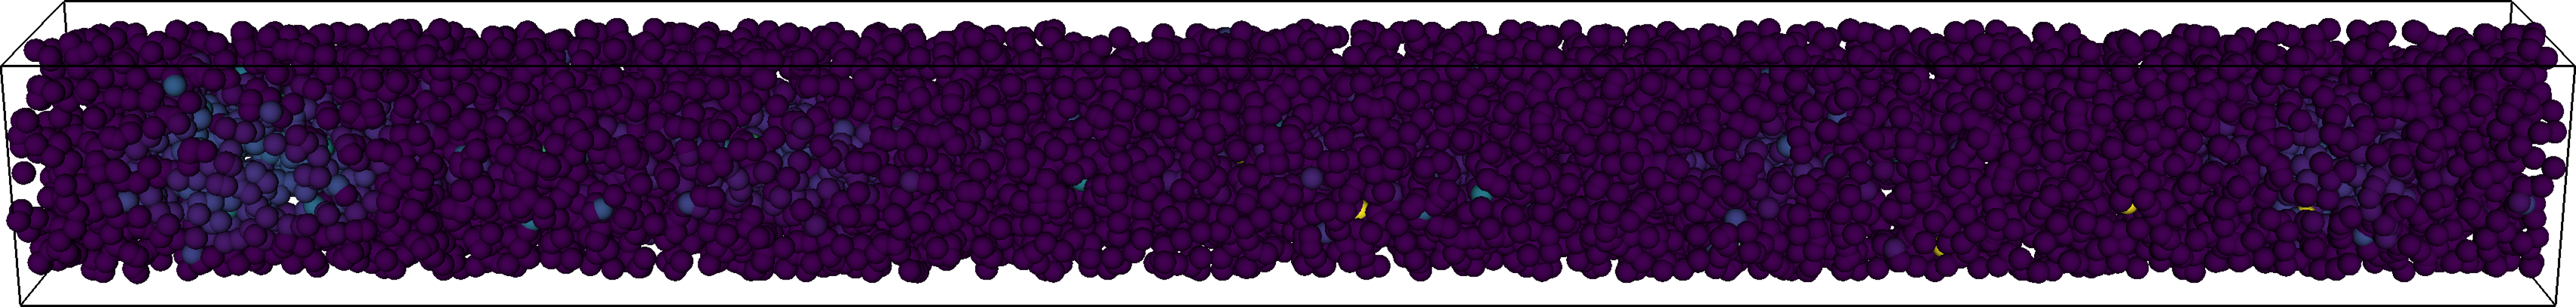
\includegraphics[width=\textwidth]{figures/tube/tube_print_0.png}} \\
  \subfloat{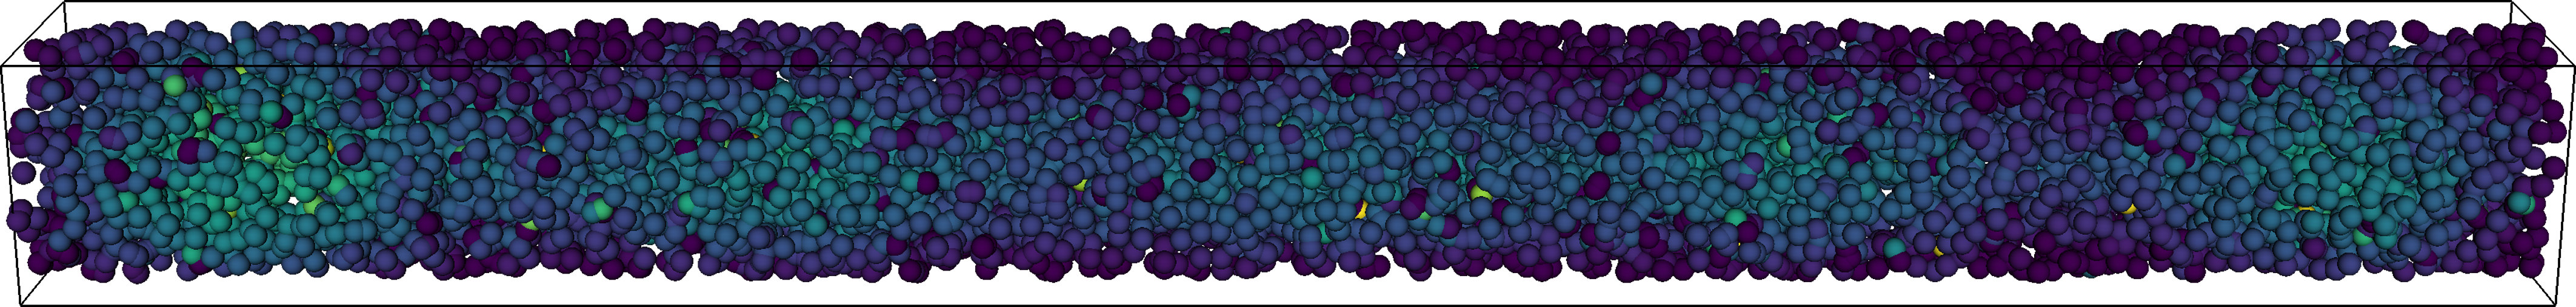
\includegraphics[width=\textwidth]{figures/tube/tube_print_1.png}} \\
  \subfloat{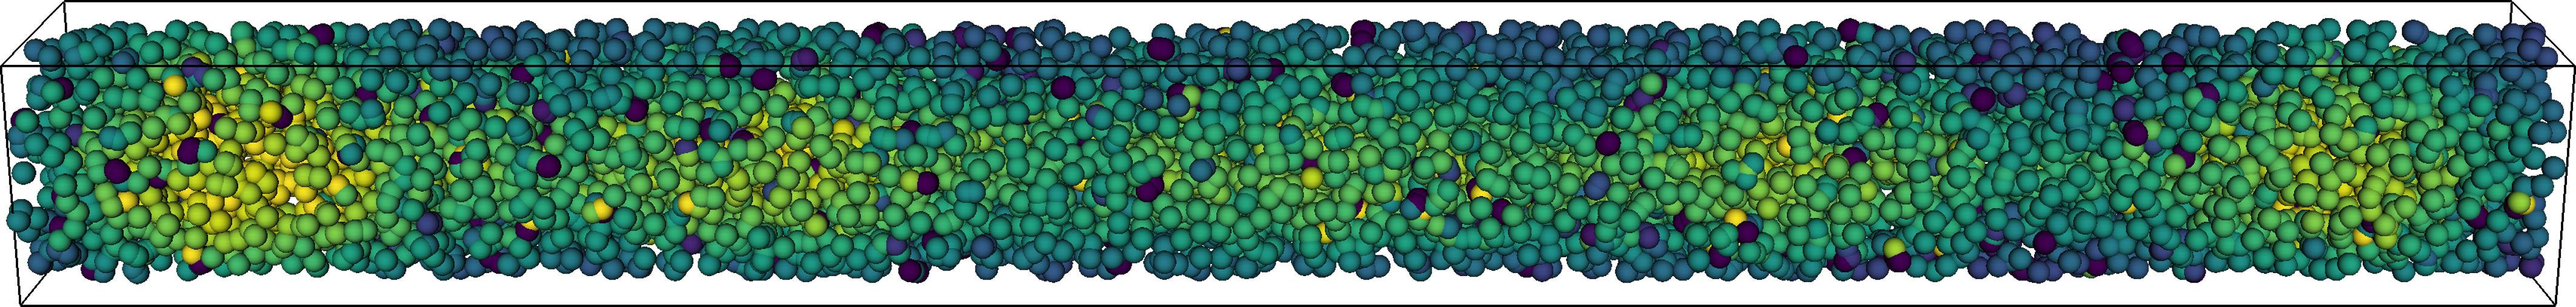
\includegraphics[width=\textwidth]{figures/tube/tube_print_2.png}} \\
  \subfloat{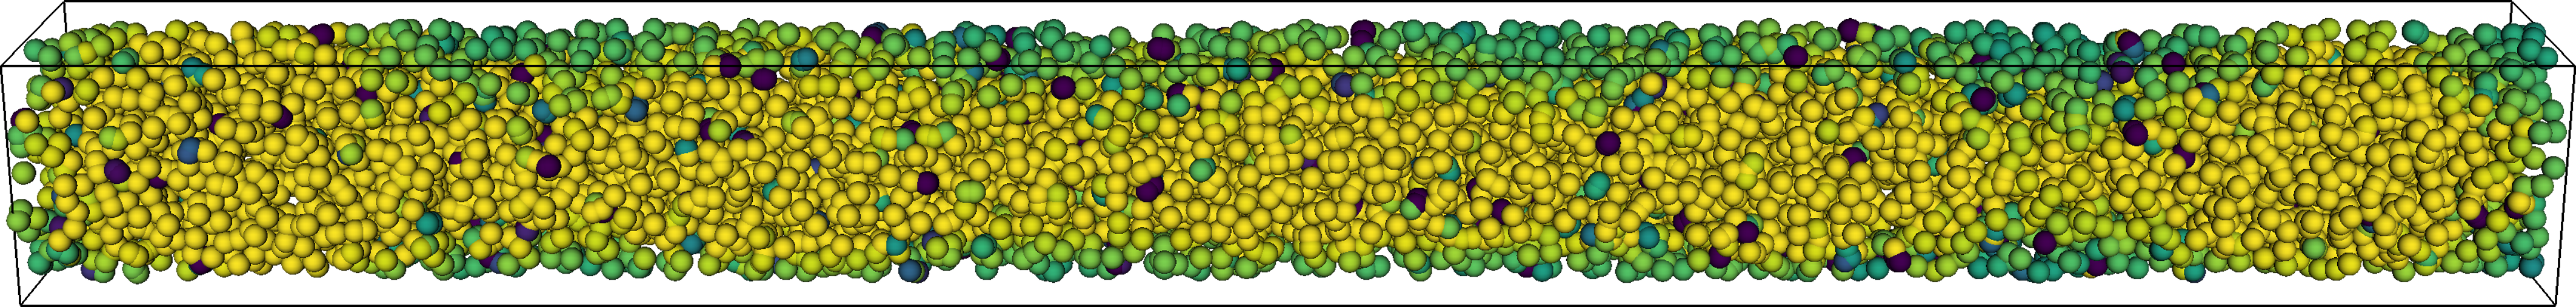
\includegraphics[width=\textwidth]{figures/tube/tube_print_3.png}}
  \caption{\label{fig:tubes}
    Time evolution of $\abs{\tilde{\rho}_{01}}^2$ for \num{10000} \qds{} randomly distributed throughout a $\SI{0.2}{\micro\meter} \times \SI{0.2}{\micro\meter} \times \SI{4}{\micro\meter}$ cylinder.
    The outlier blue/red particles correspond to adjacent \qds{} that couple strongly due to the $\vb{r}^{-3}$ term in \cref{eq:radiated envelope}.
    The $\vb{r}^{-1}$ term also produces variations in $\abs{\tilde{\rho}_{01}}^2$ on the order of $\lambda$, seen here as regions of enhanced and suppressed polarization (most apparent at the ends of the cylinder).
  }
\end{figure*}

\begin{figure}
  \centering
  \subfloat{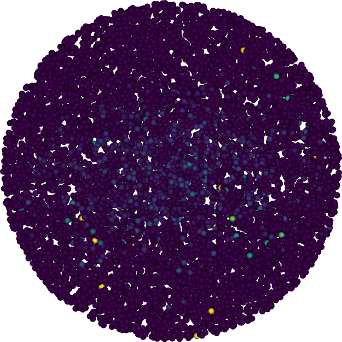
\includegraphics[width=0.25\linewidth]{figures/tube/end_print_0.png}}
  \subfloat{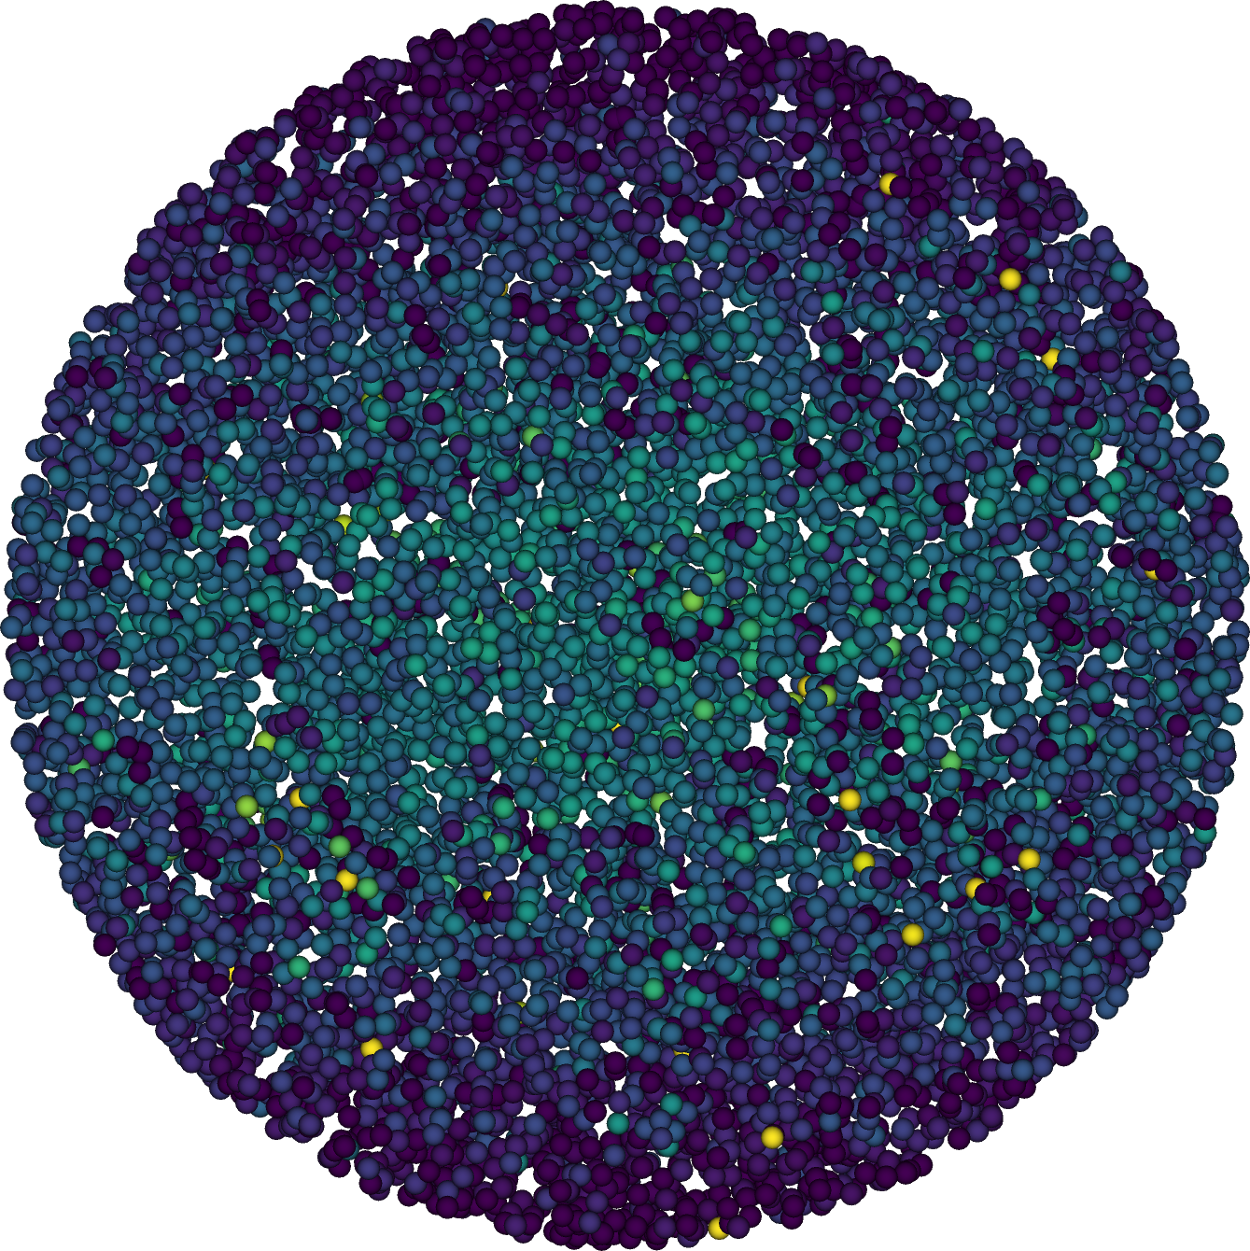
\includegraphics[width=0.25\linewidth]{figures/tube/end_print_1.png}}
  \subfloat{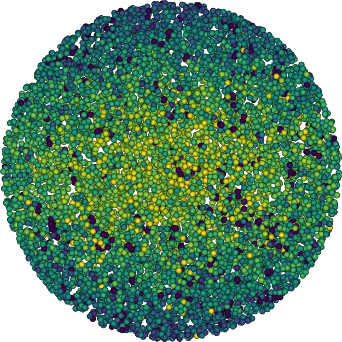
\includegraphics[width=0.25\linewidth]{figures/tube/end_print_2.png}}
  \subfloat{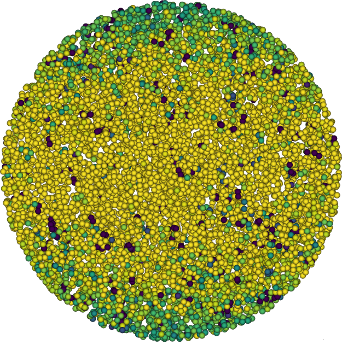
\includegraphics[width=0.25\linewidth]{figures/tube/end_print_3.png}}
  \caption{\label{fig:xy tube projection}
    \textcolor{red}{Convert to \cref{fig:tubes} projections} Projection of \cref{fig:tubes} onto the face of the cylinder.
    The uniformity of the dipole radiators breaks the cylindrical symmetry of the system, leading to regions of enhanced and suppressed polarization.
  }
\end{figure}

